% FORGE, GEM workshop (NeurIPS 2026) short-paper build.
%
% This manuscript is a condensation of paper/v1. It carries no numbers of its own: every quantitative
% statement is either typed verbatim from the v1 body or expanded from the hash-pinned macros in
% ../v1/generated/completed_evidence_macros.tex, and every table row is the same generated artifact
% the v1 manuscript inputs. Editing a value here without reissuing its artifact would break that
% correspondence.
%
% Venue contract: short papers are limited to 5 pages excluding references and appendix, must use the
% NeurIPS 2026 main-conference template with the GEM style file substituted, and are anonymous for
% double-blind review. The body therefore ends before \bibliography; everything else is appendix.

\documentclass{article}

\usepackage{GEM_workshop_2026}

\usepackage{amsmath,amssymb,amsthm}
\usepackage{algorithm}
\usepackage{algpseudocode}
\usepackage{graphicx}
\usepackage{array}
\usepackage{booktabs}
\usepackage{colortbl}
\usepackage{longtable}
\usepackage[most]{tcolorbox}
\usepackage{float}
\usepackage{xcolor}
\usepackage{url}
\usepackage[hidelinks]{hyperref}

% Figures and generated rows are read from the v1 manuscript directory so that this build and the
% full manuscript can never disagree about a number.
\graphicspath{{./}{../v1/}}

\newtheorem{theorem}{Theorem}[section]
\newtheorem{definition}[theorem]{Definition}
\newtheorem{proposition}[theorem]{Proposition}
\newtheorem{lemma}[theorem]{Lemma}
\newtheorem{corollary}[theorem]{Corollary}

% Formal statements use a quiet lavender field to separate assumptions and guarantees from the
% surrounding argument. The box may break across pages; proofs intentionally remain unboxed.
\definecolor{forgeformalbg}{HTML}{F0EFFF}
\tcbset{
  forge formal block/.style={
    enhanced jigsaw,
    breakable,
    colback=forgeformalbg,
    colframe=forgeformalbg,
    boxrule=0pt,
    arc=0pt,
    outer arc=0pt,
    boxsep=0pt,
    left=8pt,
    right=8pt,
    top=7pt,
    bottom=7pt,
    before skip=8pt,
    after skip=8pt
  }
}
\tcolorboxenvironment{definition}{forge formal block}
\tcolorboxenvironment{proposition}{forge formal block}
\tcolorboxenvironment{theorem}{forge formal block}
\tcolorboxenvironment{lemma}{forge formal block}
\tcolorboxenvironment{corollary}{forge formal block}

% Unresolved experimental results remain visually explicit until a verified artifact supplies
% the value. Never replace one of these placeholders from an unverified log or planning document.
\newcommand{\RESULTPENDING}[1]{\textbf{\textcolor{red}{[PENDING: #1]}}}
% Generated from the hash-pinned completed-evidence contract. Do not edit numerical values here.
\newcommand{\ForgeCommonRouteEvidenceCompleteComponents}{29}
\newcommand{\ForgeCommonRouteForgeAbstentionPerThousand}{$786.8\pm100.8$}
\newcommand{\ForgeCommonRouteForgeCompletePerThousand}{$0.0\pm0.0$}
\newcommand{\ForgeCommonRouteForgeExactPerThousand}{$786.8\pm100.8$}
\newcommand{\ForgeCommonRouteSelectorCompletePerThousand}{$0.7\pm0.3$}
\newcommand{\ForgeCommonRouteUnionComponents}{11{,}313}
\newcommand{\ForgeCyclicBLCIHighPP}{77.02}
\newcommand{\ForgeCyclicBLCILowPP}{71.13}
\newcommand{\ForgeCyclicBLDifferencePP}{73.67}
\newcommand{\ForgeCyclicBLRangeHighPP}{77.02}
\newcommand{\ForgeCyclicBLRangeLowPP}{71.13}
\newcommand{\ForgeCyclicBLSeedDifferencesPP}{72.85, 77.02, 71.13}
\newcommand{\ForgeCyclicLXCIHighPP}{22.01}
\newcommand{\ForgeCyclicLXCILowPP}{-3.91}
\newcommand{\ForgeCyclicLXDifferencePP}{13.15}
\newcommand{\ForgeCyclicLXRangeHighPP}{22.01}
\newcommand{\ForgeCyclicLXRangeLowPP}{-3.91}
\newcommand{\ForgeCyclicLXSeedDifferencesPP}{21.35, -3.91, 22.01}
\newcommand{\ForgeCyclicUgiCIHighPP}{49.41}
\newcommand{\ForgeCyclicUgiCILowPP}{32.00}
\newcommand{\ForgeCyclicUgiDifferencePP}{38.43}
\newcommand{\ForgeCyclicUgiRangeHighPP}{49.41}
\newcommand{\ForgeCyclicUgiRangeLowPP}{32.00}
\newcommand{\ForgeCyclicUgiSeedDifferencesPP}{32.00, 49.41, 33.89}
\newcommand{\ForgeHeldComponentAttempts}{9{,}216}
\newcommand{\ForgeHeldComponentPerThousand}{0.11}
\newcommand{\ForgeHeldComponentTotal}{1}
\newcommand{\ForgeNovelAgainstFullCount}{21{,}960}
\newcommand{\ForgeNovelAgainstFullDenominator}{26{,}235}
\newcommand{\ForgeNovelAgainstFullPercent}{83.7}
\newcommand{\ForgeNullBLCIHighPP}{78.45}
\newcommand{\ForgeNullBLCILowPP}{69.69}
\newcommand{\ForgeNullBLDifferencePP}{73.49}
\newcommand{\ForgeNullBLRangeHighPP}{78.45}
\newcommand{\ForgeNullBLRangeLowPP}{69.69}
\newcommand{\ForgeNullBLSeedDifferencesPP}{72.33, 78.45, 69.69}
\newcommand{\ForgeNullLXCIHighPP}{26.04}
\newcommand{\ForgeNullLXCILowPP}{2.51}
\newcommand{\ForgeNullLXDifferencePP}{18.10}
\newcommand{\ForgeNullLXRangeHighPP}{26.04}
\newcommand{\ForgeNullLXRangeLowPP}{2.51}
\newcommand{\ForgeNullLXSeedDifferencesPP}{26.04, 2.51, 25.75}
\newcommand{\ForgeNullUgiCIHighPP}{79.95}
\newcommand{\ForgeNullUgiCILowPP}{60.84}
\newcommand{\ForgeNullUgiDifferencePP}{67.24}
\newcommand{\ForgeNullUgiRangeHighPP}{79.95}
\newcommand{\ForgeNullUgiRangeLowPP}{60.84}
\newcommand{\ForgeNullUgiSeedDifferencesPP}{60.84, 79.95, 60.94}
\newcommand{\ForgeOffRegistryCount}{19{,}520}
\newcommand{\ForgeOffRegistryDenominator}{26{,}235}
\newcommand{\ForgeOffRegistryPercent}{74.4}
\newcommand{\ForgePotencyAUC}{0.623}
\newcommand{\ForgePotencyAUCCIHigh}{0.679}
\newcommand{\ForgePotencyAUCCILow}{0.565}
\newcommand{\ForgePotencyAttemptsPerArm}{3{,}072}
\newcommand{\ForgePotencyDifferenceCIHighPerThousand}{0.98}
\newcommand{\ForgePotencyDifferenceCILowPerThousand}{-2.28}
\newcommand{\ForgePotencyDifferencePerThousand}{-1.30}
\newcommand{\ForgePotencyNestedEligible}{82}
\newcommand{\ForgePotencyNestedExactLone}{2962}
\newcommand{\ForgePotencyNestedHigh}{23}
\newcommand{\ForgePotencyOracleBudget}{38}
\newcommand{\ForgePotencySupportEligible}{90}
\newcommand{\ForgePotencySupportExactLone}{2955}
\newcommand{\ForgePotencySupportHigh}{27}
\newcommand{\ForgePotencyTopQuartileGain}{1.177}
\newcommand{\ForgeRouteAdmitted}{255}
\newcommand{\ForgeRouteCandidates}{256}
\newcommand{\ForgeRouteCensoredComponents}{2}
\newcommand{\ForgeRouteCensoredProducts}{1}
\newcommand{\ForgeRouteCompleteComponents}{36}
\newcommand{\ForgeRouteCompleteProducts}{19}
\newcommand{\ForgeRouteComponents}{158}
\newcommand{\ForgeRouteExactLone}{256}
\newcommand{\ForgeRouteUnresolvedComponents}{120}
\newcommand{\ForgeRouteUnresolvedProducts}{236}
\newcommand{\ForgeSemanticBLTokenCIHighPP}{5.60}
\newcommand{\ForgeSemanticBLTokenCILowPP}{-2.18}
\newcommand{\ForgeSemanticBLTokenDifferencePP}{2.00}
\newcommand{\ForgeSemanticBLTokenPercent}{37.70}
\newcommand{\ForgeSemanticBLTokenRangeHighPP}{5.60}
\newcommand{\ForgeSemanticBLTokenRangeLowPP}{-2.18}
\newcommand{\ForgeSemanticBLTokenSeedDifferencesPP}{-2.18, 5.60, 2.57}
\newcommand{\ForgeSemanticFactualPercent}{39.69}
\newcommand{\ForgeSemanticForwardRoleCIHighPP}{1.69}
\newcommand{\ForgeSemanticForwardRoleCILowPP}{0.29}
\newcommand{\ForgeSemanticForwardRoleDifferencePP}{0.82}
\newcommand{\ForgeSemanticForwardRolePercent}{38.87}
\newcommand{\ForgeSemanticForwardRoleRangeHighPP}{1.69}
\newcommand{\ForgeSemanticForwardRoleRangeLowPP}{0.29}
\newcommand{\ForgeSemanticForwardRoleSeedDifferencesPP}{0.29, 1.69, 0.49}
\newcommand{\ForgeSemanticLXTokenCIHighPP}{27.47}
\newcommand{\ForgeSemanticLXTokenCILowPP}{14.06}
\newcommand{\ForgeSemanticLXTokenDifferencePP}{22.60}
\newcommand{\ForgeSemanticLXTokenPercent}{17.09}
\newcommand{\ForgeSemanticLXTokenRangeHighPP}{27.47}
\newcommand{\ForgeSemanticLXTokenRangeLowPP}{14.06}
\newcommand{\ForgeSemanticLXTokenSeedDifferencesPP}{14.06, 26.27, 27.47}
\newcommand{\ForgeSemanticNullCoordinatesCIHighPP}{37.24}
\newcommand{\ForgeSemanticNullCoordinatesCILowPP}{34.28}
\newcommand{\ForgeSemanticNullCoordinatesDifferencePP}{36.07}
\newcommand{\ForgeSemanticNullCoordinatesPercent}{3.62}
\newcommand{\ForgeSemanticNullCoordinatesRangeHighPP}{37.24}
\newcommand{\ForgeSemanticNullCoordinatesRangeLowPP}{34.28}
\newcommand{\ForgeSemanticNullCoordinatesSeedDifferencesPP}{37.24, 34.28, 36.69}
\newcommand{\ForgeSemanticReverseRoleCIHighPP}{8.27}
\newcommand{\ForgeSemanticReverseRoleCILowPP}{1.37}
\newcommand{\ForgeSemanticReverseRoleDifferencePP}{4.49}
\newcommand{\ForgeSemanticReverseRolePercent}{35.20}
\newcommand{\ForgeSemanticReverseRoleRangeHighPP}{8.27}
\newcommand{\ForgeSemanticReverseRoleRangeLowPP}{1.37}
\newcommand{\ForgeSemanticReverseRoleSeedDifferencesPP}{8.27, 1.37, 3.84}
\newcommand{\ForgeSynthesisCanonicalRepresentatives}{56}
\newcommand{\ForgeSynthesisChangedIdentities}{8}
\newcommand{\ForgeSynthesisGuidanceStrength}{0.25}
\newcommand{\ForgeSynthesisGuidedReady}{2}
\newcommand{\ForgeSynthesisPosthocReady}{3}
\newcommand{\ForgeSynthesisTerminalParticles}{64}
\newcommand{\ForgeUgiRetentionCIHighPP}{61.82}
\newcommand{\ForgeUgiRetentionCILowPP}{41.24}
\newcommand{\ForgeUgiRetentionDifferencePP}{53.26}
\newcommand{\ForgeUgiRetentionRangeHighPP}{61.82}
\newcommand{\ForgeUgiRetentionRangeLowPP}{41.24}
\newcommand{\ForgeUgiRetentionSeedDifferencesPP}{41.24, 56.71, 61.82}


% Appendix generated-structure atlas. The hash-pinned row file carries structures and SMILES only
% and defers every length, rule and type style to the definitions below, so the appendix can be
% retuned without reissuing a provenance artifact.
\definecolor{atlasrule}{gray}{0.74}
\definecolor{atlasink}{gray}{0.42}
\newlength{\atlasgraphwidth}
\newlength{\atlasviewwidth}
\newlength{\atlasgraphheight}
\newlength{\atlasviewheight}
\newlength{\atlasrowheight}
\newlength{\atlasrankwidth}
\newlength{\atlassmilesskip}
% Every column is pinned to a stated width, so the alignment cannot be widened past \textwidth by a
% heading or an index label. These must sum with the three gutters and the divider in the column
% specification: 5mm + 1.8mm + 0.545 + 2.8mm + 0.5pt + 2.8mm + 0.3648 = \textwidth.
\setlength{\atlasrankwidth}{5mm}
\setlength{\atlasgraphwidth}{0.545\textwidth}
\setlength{\atlasviewwidth}{0.3648\textwidth}
\setlength{\atlasgraphheight}{2.45cm}
\setlength{\atlasviewheight}{3.20cm}
% Rows are struck to a common height that exceeds both panels: the surplus is the air between
% structures, and holding it inside the row keeps the column divider unbroken and keeps the
% multipage break in the same place for every row rather than following a wrapped SMILES string.
\setlength{\atlasrowheight}{4.00cm}
\setlength{\atlassmilesskip}{2.4mm}
\newcommand{\atlassmilesstyle}{\scriptsize\ttfamily\color{atlasink}}
\newcommand{\atlasrank}[1]{%
  \makebox[\atlasrankwidth]{\raisebox{-0.5\height}{\footnotesize\color{atlasink}#1}}}
\newcommand{\atlashead}[2]{\makebox[#1]{\footnotesize\scshape #2}}

\title{FORGE: Reaction-Grounded Generative Design of Ionizable Lipids}

\author{Anonymous authors\\Paper under double-blind review}

\begin{document}

\maketitle

\begin{abstract}
Ionizable lipids are central to RNA delivery, yet their discovery still largely relies on modular
synthesis and screening of molecular libraries whose constituent chemistry is chosen in advance. De
novo generation could expand this design space, but opening molecular identity risks severing the
reaction semantics that make a design experimentally interpretable and assemblable. We introduce
FORGE (\textbf{F}low-matched, \textbf{O}pen-ended, \textbf{R}oute-resolved \textbf{G}eneration and
\textbf{E}xploration), a reaction-grounded generative framework that uses known reaction chemistry
as the coordinate system for molecular generation. Reaction programs specify precursor roles, reaction-core
positions, transformation order, and coarse molecular architecture, defining how regions of the
final molecule participate in synthesis while leaving their molecular identities open. A conditional
discrete flow then generates the complete molecular realization at atom-and-bond resolution without
component identifiers, stored precursor graphs, or fragment tokens. Across Ugi, repeated aza-Michael
addition, and repeated reductive amination, FORGE achieves exact level-one transform-consistent
yields of $78.7\%$, $77.5\%$, and $31.3\%$, substantially outperforming matched whole-graph
generation followed by post-hoc reaction filtering. Across all three programs, FORGE also generated exact-L1
products with recovered precursor identities beyond the corresponding training component catalogues,
a capability unavailable to finite catalogue assemblers by construction. FORGE
therefore uses reaction knowledge to preserve assembly semantics while opening molecular identity to
de novo generation.
\end{abstract}

\section{Introduction}

Lipid nanoparticles (LNPs) deliver nucleic-acid therapeutics including small interfering RNA, mRNA
vaccines and \emph{in vivo} genome-editing reagents
\citep{adams2018patisiran,polack2020safety,baden2021efficacy,gillmore2021crispr}. Within each LNP,
the ionizable lipid supports nucleic-acid complexation and influences particle assembly and
endosomal escape, making its structure a central determinant of function
\citep{cullis2017lipid,hou2021lipid}. Small changes to headgroup and hydrophobic structure can
substantially alter delivery, yet their effects depend on the complete molecular context and do not
consistently follow simple design rules
\citep{cheng2020selective,han2021ionizable,hatit2023nanoparticle}. Discovery therefore commonly
proceeds by defining modular precursor libraries, synthesizing combinations and screening the
resulting LNPs experimentally
\citep{akinc2008combinatorial,love2010lipidlike,li2024accelerating,xu2024agile}. This workflow
preserves experimental tractability, but largely fixes the molecular vocabulary of the search before
design begins.

De novo generative modeling offers a way beyond this ceiling, but reaction grounding creates a
representational problem. Synthesis-aware generators commonly encode chemical feasibility by
constructing molecules through predefined reactions and reactant inventories
\citep{gao2022amortized,koziarski2024rgfn,cretu2025synflownet,rekesh2026syncogen}. This makes
chemistry part of the generative action space and preserves an explicit assembly path, but also ties
reachable molecular identity to the supplied vocabulary. Generic whole-molecule generators have the
complementary strength: they can generate new molecular identities, but do not by themselves
preserve which regions must function as particular precursors or which transformations should
assemble them \citep{qin2025defog,lee2025genmol}. A complementary line of work evaluates
synthesizability after generation rather than encoding construction directly into the generative
state \citep{gao2020synthesizability}. Recent work has also begun to explore de novo generative
modeling specifically for ionizable lipids \citep{ou2024deep,maganti2026synthesis}. We ask whether known
reaction chemistry can instead organize an open generative state without specifying the molecular
structures that occupy it. Our premise is that reaction grounding need not require component
enumeration: reaction knowledge can provide semantic coordinates that determine how molecular
regions participate in construction while leaving their identities generative.

We introduce FORGE (\textbf{F}low-matched, \textbf{O}pen-ended, \textbf{R}oute-resolved
\textbf{G}eneration and \textbf{E}xploration), a reaction-grounded generative framework that uses
known reaction chemistry as the coordinate system for molecular generation. A reaction program specifies the assembly chemistry,
precursor roles, reaction-core positions, transformation order and coarse molecular architecture,
but not precursor identities. Conditioned on this program, a discrete flow generates the complete
molecular realization at atom-and-bond resolution without component identifiers, stored precursor
graphs or fragment tokens. Because reaction semantics are preserved in the generative state, each
completed molecule can be decomposed into the precursors implied by its program and the specified
assembly reaction replayed exactly. Precursors that are not directly available are then assessed
recursively for upstream preparation, yielding a complete evidence-qualified computational synthesis
dossier or an explicit unresolved or search-censored outcome. We evaluate this formulation across a Ugi
three-component reaction, repeated aza-Michael addition and repeated reductive amination. These experiments test generalization across specified reaction programs rather than
zero-shot support for arbitrary chemistry. Our contributions are threefold. First, we formulate
reaction-grounded whole-graph generation in which reaction programs provide semantic coordinates
while molecular identity remains generative at atom-and-bond resolution. Second, matched controls
across three assembly programs show that reaction semantics substantially increase exact
transform-consistent generation relative to whole-graph generation followed by post-hoc filtering.
Third, FORGE leaves precursor identity open rather than restricting generation to a finite component
vocabulary; across all three programs, this yields exact-assembly products with recovered precursor
identities beyond the corresponding training catalogues.


\section{FORGE}

\begin{figure}[tb]
\centering
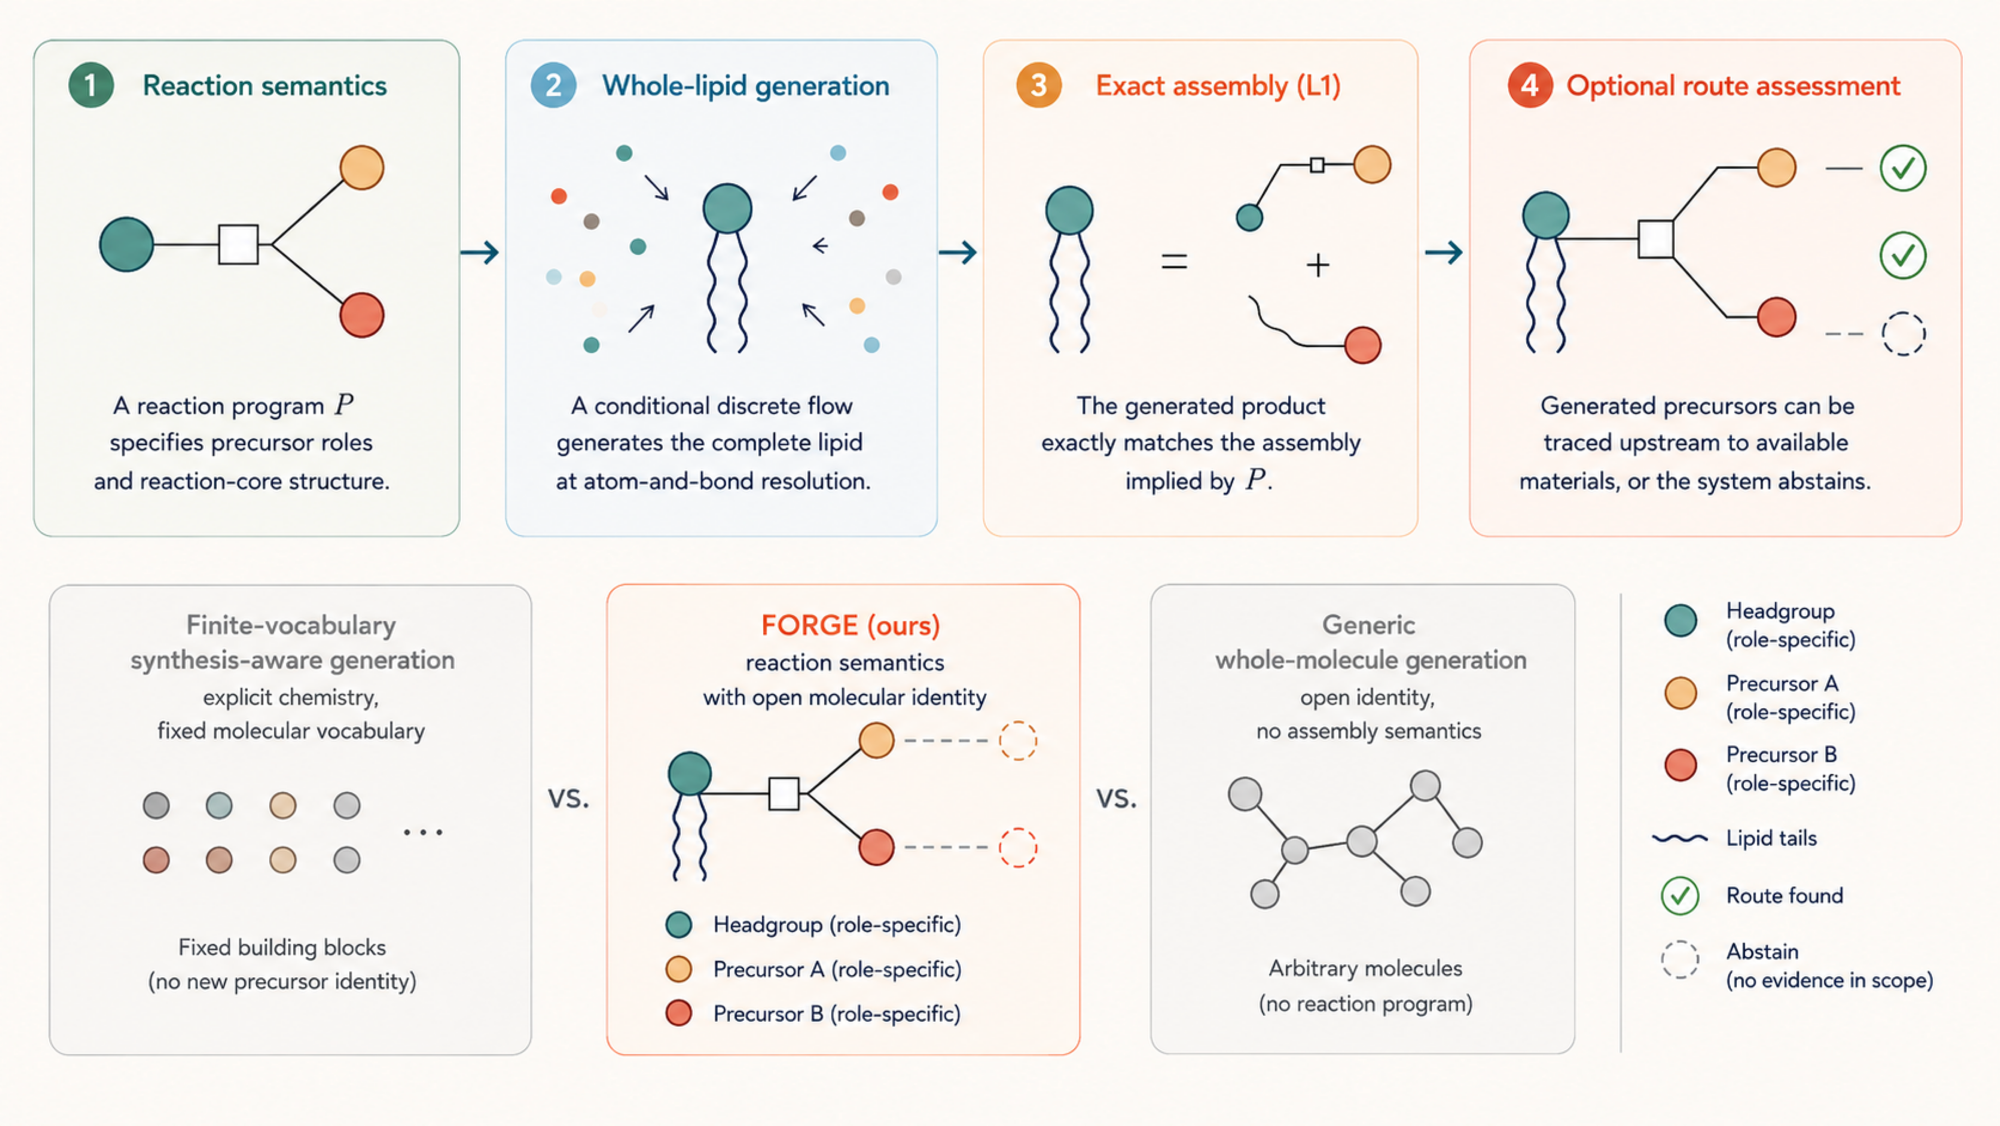
\includegraphics[width=\textwidth]{figures/forge_framework_v2/forge_framework.png}
\caption{\textbf{FORGE uses reaction chemistry as the coordinate system for molecular
generation.} A reaction program specifies precursor roles and reaction-core structure without fixing
molecular identities; a conditional discrete flow generates the complete lipid, and exact assembly
verification requires forward reconstruction from the implied precursors. Optional downstream routing
assesses unavailable precursors or abstains. Bottom, FORGE combines explicit reaction semantics with
generated molecular identity. Colors denote semantic roles, not component identities.}
\label{fig:forge-framework}
\end{figure}


We formulate ionizable-lipid design as conditional generation under a specified reaction program,
while leaving precursor identities unspecified.
Let $G\in\mathcal{G}$ denote a complete ionizable-lipid graph and $P\in\mathcal{P}$ a reaction
program specifying the assembly chemistry, precursor roles, reaction-core positions, and
transformation order.
FORGE models the conditional distribution $p_\theta(G\mid P)$ without access to precursor
identifiers, stored component graphs, or fragment tokens.
Given $P$, FORGE generates a complete molecular graph $G$. A downstream bounded program constructor
then returns a recursive synthesis program $T$ or an explicit abstention outcome. Writing
$\mathfrak{T}$ for the space of recursive synthesis programs and $\bot$ for that abstention,
\begin{equation}
    G\sim p_\theta(\cdot\mid P),
    \qquad
    T=\mathcal{A}(G,P)\in\mathfrak{T}\cup\{\bot\},
\end{equation}
where $\mathcal{A}$ is the bounded program constructor that verifies the final assembly, searches for
preparation routes to unavailable precursors, and checks terminal supplier evidence. $P$ and
$\mathcal{A}$ act at different stages: $P$ guides the generation of $G$, whereas $\mathcal{A}$
assesses the completed graph without modifying it. A pair $(G,T)$ is designated route-complete only
when $G$ passes molecular and exact-assembly verification and every required precursor traces to an
available starting material; otherwise the route assessor abstains.

A reaction program is a tuple $P=(c,d,\mathbf{r},\mathbf{k},M)$, where $c$ identifies the ordered
assembly chemistry, $d$ is the program depth, $\mathbf{r}$ assigns precursor roles, $\mathbf{k}$
marks reaction-core positions, and $M$ specifies coarse per-role morphology as four integers per
role: exterior atom count, junction budget, cycle rank and attachment count. $M$ sets only coarse
structural constraints; the model generates the exact topology, atoms and bonds of each region.
FORGE samples $M$ from a training-fold morphology prior and then generates $G$ conditioned on the
resulting program, so that
$p_\theta(G,M\mid c)=p_{\mathrm{prog}}(M\mid c)\,p_\theta(G\mid M,c)$.
For each graph position $i$, FORGE combines learned embeddings of program identity, program depth,
precursor role and reaction-core position,
$h_i^P=\operatorname{LN}(e_c(c)+e_d(d)+e_r(r_i)+e_k(k_i))$.
These coordinates tell the generator which precursor role each position plays and whether it lies in
the reaction core, but not which molecular structure should occupy that role.

The framework comprises three core stages followed by optional downstream route assessment: the
program specifies roles, core positions, order and coarse morphology; a conditional discrete flow
generates every atom, bond and topology state under it; a reverse transform decomposes the product
and the corresponding forward transform must reconstruct it exactly; and precursors that are not
already available may then be assessed recursively, with abstention when the route evidence is
incomplete. Generation operates on a sparse tree-plus-closure encoding. Let
$X_G=(\mathbf{a},\boldsymbol{\pi},\mathbf{b},\mathbf{e}^{L},\mathbf{e}^{R},\mathbf{z})$
be the categorical graph state, with $\mathbf{a}$ atom states, $\boldsymbol{\pi}$ parent pointers,
$\mathbf{b}$ spanning-tree bond states, $\mathbf{e}^{L}$ and $\mathbf{e}^{R}$ closure endpoints and
$\mathbf{z}$ closure-bond states. The decoder is surjective onto the declared graph space
$\mathfrak{G}_{N_{\max},K}$, here $N_{\max}=194$ and $K=3$, so every graph within the declared atom,
bond and size support is representable. This is a statement about architectural support, not about
reaction consistency or probability under a trained model.

The chemistry adapter marks the atom, pointer and bond states that $P$ fixes. FORGE holds those
constant while corrupting the remaining states along the linear probability path and predicting their
clean values from $(X_t,t,P)$. Writing $\mathcal{Q}$ for the six state families,
$m_j^{(q)}(P)\in\{0,1\}$ for whether coordinate $j$ remains variable under $P$, and
$\mu_{\mathrm{bal}}$ for the frozen program-balanced training distribution, and
$\ell^{(q)}_j(\theta)=-\log p_\theta(X_{G,j}^{(q)}\mid X_t,t,P)$ for the per-coordinate denoising
term, FORGE minimizes
\begin{equation}
    \mathcal{L}_{\mathrm{FORGE}}(\theta)
    = \mathbb{E}_{\substack{
        (G,P)\sim\mu_{\mathrm{bal}},\;
        t\sim\mathcal{U}(0,1),\;
        X_t\sim p_t(\cdot\mid X_G,P)}}
    \left[\,
        \sum_{q\in\mathcal{Q}}
        \lambda_q\,
        \frac{\sum_j m_j^{(q)}(P)\,\ell^{(q)}_j(\theta)}
        {\max\!\left\{1,\sum_j m_j^{(q)}(P)\right\}}
    \right],
\end{equation}
where $\lambda_q$ weights family $q$ and a family with no variable coordinates contributes zero loss.
The corruption and sampling operators project every intermediate state onto the program-fixed
coordinates, so those coordinates are invariant by construction while the masked objective learns the
conditional clean-state distributions of the remainder. This is the precise sense in which reaction
semantics enter generation rather than filtering: the program fixes which coordinates the model is
never permitted to resample. Appendix~\ref{app:forge} gives the sampler, verifier and bounded route
assessor in full, and Appendix~\ref{app:theory} the representation, invariance, sampling-efficiency
and termination results.

\section{Results}

We evaluate three assembly programs, with Ugi as the deeply supervised case, repeated aza-Michael
addition as a second family, and repeated reductive amination as a lighter stress test, across four
matched training arms: Ugi-only conditioning, shared conditioning, shared training without program
information, and shared training with cyclically incorrect program labels. All arms share
architecture, optimization budget and attempts per program, and we evaluate the prespecified final
checkpoint from each of three independent seeds. The primary metric is exact-L1 yield per generation
attempt: generated graphs passing molecular validity, program-aware decomposition and exact forward
replay, divided by total attempts. Training uses only the component-disjoint training folds, and
held-out products neither enter training nor select checkpoints. Generated molecules are not treated
as independent replicates. Appendix~\ref{app:results} states the full protocol, including the
external-baseline admission rules.

\subsection{One shared model learns multiple assembly programs}
Across 3,072 held-out generation attempts per program in each of three independent training seeds,
the final conditioned model achieved exact-L1 yields of $78.7\pm10.1\%$ for Ugi
($72.3\%$, $90.3\%$ and $73.5\%$ by seed), $77.5\pm3.7\%$ for repeated aza-Michael
addition ($76.5\%$, $81.5\%$ and $74.3\%$), and $31.3\pm14.3\%$ for repeated reductive
amination ($38.6\%$, $14.8\%$ and $40.4\%$) (mean $\pm$ sample standard deviation;
Table~\ref{tab:gem-shared-programs}).
Exact forward-replay precision was $100\%$ in every program and seed, but mean decomposition
ambiguity was $54.9\%$ for aza-Michael addition and $74.1\%$ for reductive amination, and the latter
varied substantially between seeds. Relative to Ugi-only training ($25.4\pm12.0\%$), shared
conditioning increased Ugi exact-L1 yield to $78.7\pm10.1\%$, a
\ForgeUgiRetentionDifferencePP-point improvement (95\% paired-seed interval
\ForgeUgiRetentionCILowPP{} to \ForgeUgiRetentionCIHighPP), met every prespecified Ugi-retention gate,
and produced zero fixed-state violations and zero support overflows across 27,648 held-out attempts.
One conditional flow can therefore learn the three specified reaction-program coordinates without
erasing the deeply supported Ugi behavior.

\begin{table}[tb]
\caption{\textbf{One shared conditional flow learns three ionizable-lipid assembly programs.}
Exact-L1 yield and decomposition/replay statistics are reported as mean $\pm$ sample standard
deviation across three independent training seeds. Results are never pooled across programs. Per-seed
results and full matched controls are reported in Appendix~\ref{app:results}.}
\label{tab:gem-shared-programs}
\centering
\small
\setlength{\tabcolsep}{4.6pt}
\begin{tabular}{@{}lcccc@{}}
\toprule
Program & FORGE conditioned & Shared null & Cyclic program & Decomposition / replay (\%) \\
\midrule
Ugi & $78.7\pm10.1$ & $11.4\pm1.1$ & $40.2\pm0.7$ & 90.7/100.0 \\
Aza-Michael & $77.5\pm3.7$ & $4.0\pm0.8$ & $3.8\pm0.6$ & 100.0/100.0 \\
Reductive amination & $31.3\pm14.3$ & $13.2\pm1.3$ & $18.1\pm0.8$ & 84.3/100.0 \\
%
\end{tabular}
\end{table}

\subsection{Reaction semantics alter generation rather than merely filtering its output}
Under matched attempt budgets, conditioned generation produced 786.8, 774.6 and 312.7 exact-L1
products per 1,000 attempts for Ugi, repeated aza-Michael and repeated reductive amination, compared
with 114.4, 39.7 and 131.7 for matched null generation followed by post-hoc filtering. The paired
conditioned-minus-post-hoc differences were \ForgeNullUgiDifferencePP{} percentage points for Ugi
(95\% interval \ForgeNullUgiCILowPP{} to \ForgeNullUgiCIHighPP), \ForgeNullBLDifferencePP{} for
aza-Michael (\ForgeNullBLCILowPP{} to \ForgeNullBLCIHighPP), and \ForgeNullLXDifferencePP{} for
reductive amination (\ForgeNullLXCILowPP{} to \ForgeNullLXCIHighPP). A cyclic control that retained
precursor roles, reaction-core coordinates and program depth but assigned the wrong reaction identity
changed exact-L1 yield by \ForgeCyclicUgiDifferencePP{} percentage points for Ugi
(\ForgeCyclicUgiCILowPP{} to \ForgeCyclicUgiCIHighPP), \ForgeCyclicBLDifferencePP{} for aza-Michael
and \ForgeCyclicLXDifferencePP{} for reductive amination. A separate fixed-network
inference-time intervention similarly showed that nulling the program coordinates sharply reduced Ugi
exact-L1 yield, confirming that the semantic coordinates affect generation rather than only
downstream assessment (Appendix~\ref{app:semantic-intervention}).

\subsection{Whole-graph generation produces precursor identities beyond a finite vocabulary}
Table~\ref{tab:ugi-common-benchmark} compares FORGE with external synthesis-aware generators, matched
controls and a finite-catalogue oracle under one common Ugi benchmark, normalizing every yield by
generation attempts. The learned finite-inventory selector reached $1000.0\pm0.0$ exact-L1 products
per 1,000 attempts with zero open-ended component generation, imposed by its finite action space,
whereas FORGE produced $786.8\pm100.8$ exact-L1 products and
$751.2\pm80.2$ unique exact-L1 products per 1,000 attempts. All of the latter were open-ended
against the method-visible training catalogue; against the full training catalogue the open-ended
yield was $729.3$ per 1,000 (Table~\ref{tab:catalogue-comparison}). Among open-ended external generators, unconditional DeFoG produced $280.6\pm26.6$ exact-L1
products and recovered held components at $15.5\pm2.4$ per 1,000 attempts against $0.1\pm0.2$ for
FORGE; GenMol/SAFE produced $627.5\pm6.2$ valid connected outputs but no exact Ugi-L1 product, and
RGFN emitted no admissible output under the strict native contract. Against the train-only assembler,
FORGE effective component counts were 320.8, 156.9 and 102.9 versus 86.4, 23.4 and 16.9. Reaction
consistency, open-ended identity generation and recovery of reserved components therefore trade off
separately.

\begin{table}[tb]
\caption{\textbf{FORGE combines exact Ugi assembly with precursor identities beyond a finite
training vocabulary.}
All methods are evaluated under the common component-disjoint split, three-seed attempt budget and
exact-L1 verifier, as mean $\pm$ sample standard deviation per 1,000 generation attempts. Open-ended
yield denotes exact-L1 products with a verifier-returned precursor constitution absent from the
method-visible training catalogue; the stricter yield against the full training catalogue is
reported in Table~\ref{tab:catalogue-comparison}. $\dagger$ denotes a structural zero for methods
restricted to finite component inventories. N/E, not estimable. No published values from the original
baseline papers are inserted. Full admission rules and seed-level results are reported in
Appendix~\ref{app:results}.}
\label{tab:ugi-common-benchmark}
\centering
\scriptsize
\setlength{\tabcolsep}{2.2pt}
% The generated rows put long italic group labels in column 1. Left unconstrained they set the
% table's natural width, and \resizebox then shrinks every number to about 5pt. Fixing column 1
% lets the numeric columns, not the labels, decide the scale.
%
% Those group labels are the only use of \textit in the generated rows, and every data row is
% plain. Italic alone, wrapped inside a 3.45cm column, reads as another method name. Rendering
% them as bold small caps in a zero-width left-aligned box separates the groups without editing the
% artifact. The box lets a long label run across the numeric cells of its own row, which are empty,
% so a group title sets on one line instead of wrapping to four inside a 3.45cm column. A shaded
% \rowcolor cannot be used here: colortbl needs it before the row begins, and expanding it from
% inside the first cell raises "Misplaced \noalign".
\begingroup
\renewcommand{\textit}[1]{\makebox[0pt][l]{\textbf{\scshape #1}}}
\begin{tabular}{@{}>{\raggedright\arraybackslash}p{3.45cm}cccccc@{}}
\toprule
Method & Valid & Exact L1 & Unique L1 & Open-ended & Held-comp. & Diversity \\
\midrule
\textit{Reaction-space external baselines} & & & & & & \\
RGFN & $0.0\pm0.0$ & $0.0\pm0.0$ & $0.0\pm0.0$ & $0.0\pm0.0^{\dagger}$ & $0.0\pm0.0$ & N/E \\
\textit{Generic whole-molecule external baselines with common post-hoc assessment} & & & & & & \\
DeFoG unconditional & $346.5\pm42.3$ & $280.6\pm26.6$ & $280.6\pm26.6$ & $280.6\pm26.6$ & $15.5\pm2.4$ & $0.727\pm0.014$ \\
GenMol/SAFE & $627.5\pm6.2$ & $0.0\pm0.0$ & $0.0\pm0.0$ & $0.0\pm0.0$ & $0.0\pm0.0$ & $0.873\pm0.009$ \\
\textit{Matched controls and formulation baselines} & & & & & & \\
Learned inventory selector & $1000.0\pm0.0$ & $1000.0\pm0.0$ & $849.5\pm13.7$ & $0.0\pm0.0^{\dagger}$ & $0.0\pm0.0$ & $0.717\pm0.001$ \\
Finite catalogue oracle & $1000.0\pm0.0$ & $1000.0\pm0.0$ & $837.6\pm8.2$ & $0.0\pm0.0^{\dagger}$ & $0.0\pm0.0$ & $0.719\pm0.000$ \\
Shared-null + post-hoc & $194.7\pm15.6$ & $114.4\pm10.9$ & $108.5\pm9.7$ & $108.5\pm9.7$ & $0.4\pm0.2$ & $0.754\pm0.014$ \\
FACT-matched & $60.8\pm20.2$ & $52.0\pm15.6$ & $50.8\pm14.4$ & $50.8\pm14.4$ & $0.0\pm0.0$ & $0.667\pm0.009$ \\
FACT-generous & $500.7\pm213.8$ & $296.7\pm186.0$ & $288.3\pm175.3$ & $288.3\pm175.3$ & $0.1\pm0.2$ & $0.774\pm0.007$ \\
FORGE Transformer & $866.0\pm90.2$ & $786.8\pm100.8$ & $751.2\pm80.2$ & $751.2\pm80.2$ & $0.1\pm0.2$ & $0.621\pm0.011$ \\
%
\end{tabular}
\endgroup
\end{table}

Accepted upstream transformations must reconstruct their targets under the corresponding forward
reaction, and terminal branches must close under the frozen material-evidence policy. Because route
coverage depends on the available reaction and procurement evidence, unresolved outputs are treated
as abstentions rather than evidence of unsynthesizability; full route-assessment details are given in
Appendix~\ref{app:results}.



\begin{figure}[tb]
\centering
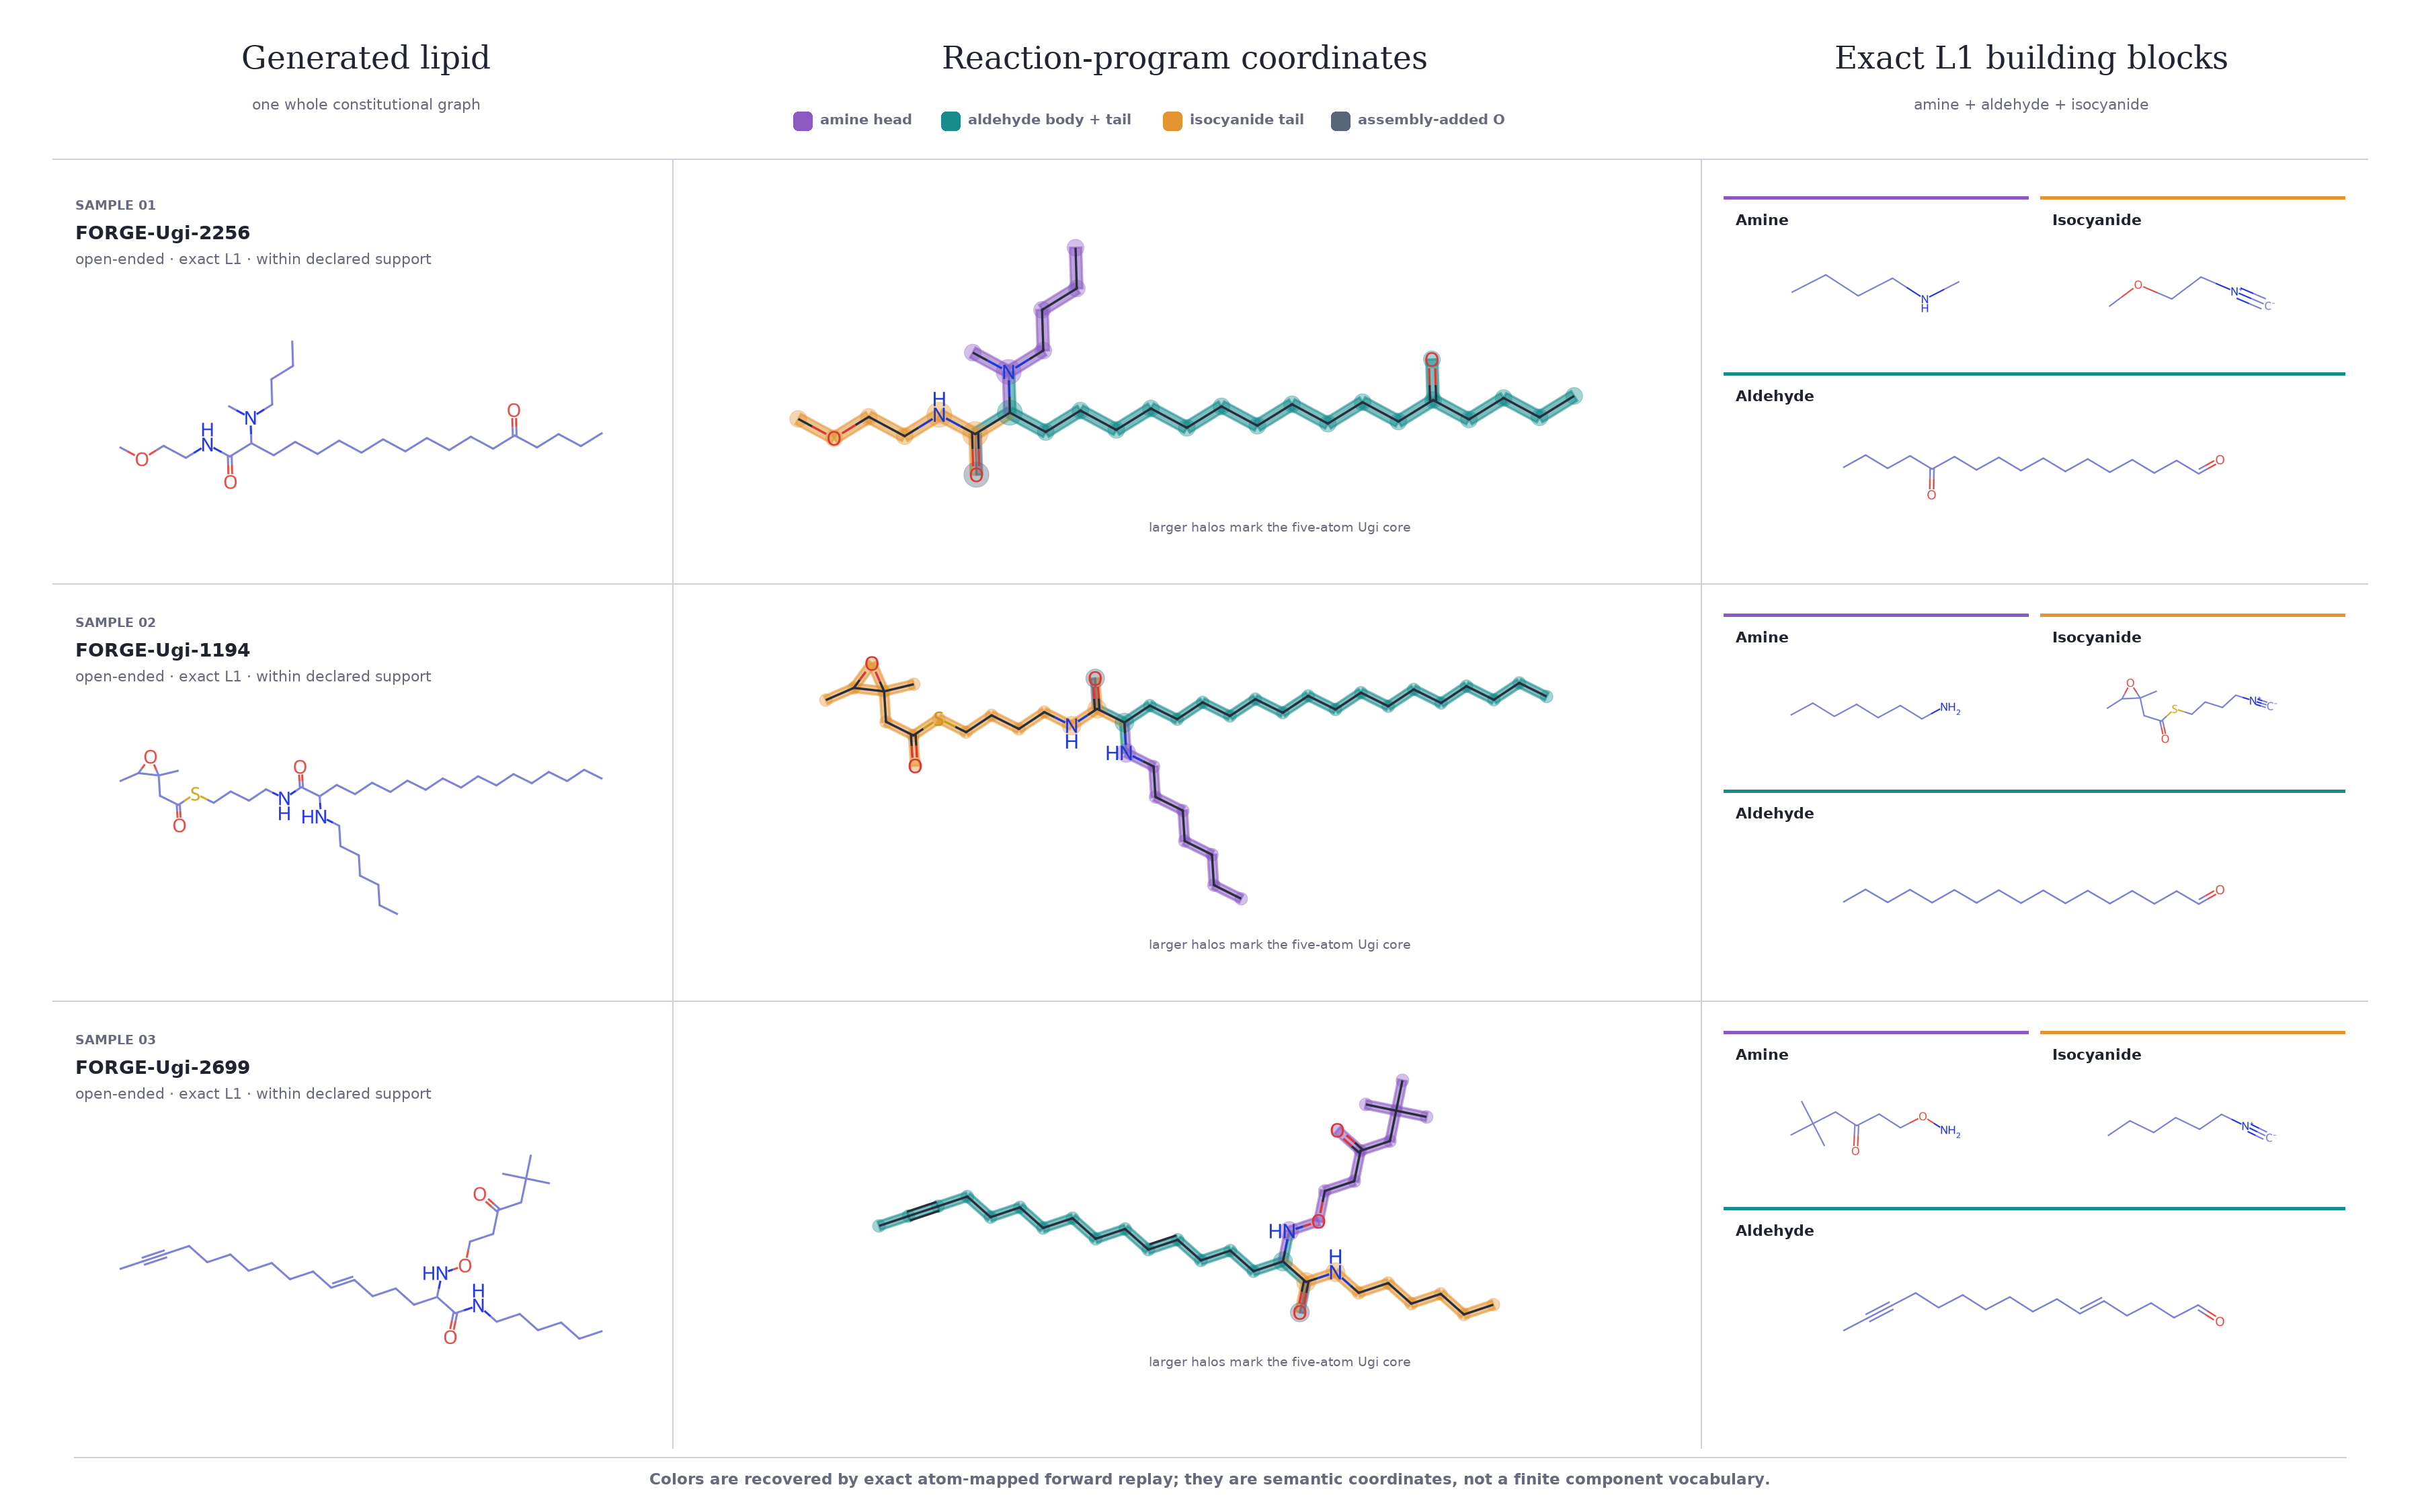
\includegraphics[width=0.72\textwidth]{figures/forge_generated_samples_v2/forge_generated_samples.png}
\footnotesize
\caption{\textbf{Deterministic examples of open-ended FORGE ionizable-lipid graphs.}
Each row is one seed-0 Ugi product with a unique exact-L1 decomposition and a recovered precursor
constitution outside the method-visible training inventory. Left, the graph sampled jointly by FORGE;
center, precursor origins recovered by exact atom-mapped forward replay, halos marking the Ugi core;
right, the exact precursor constitutions returned by the verifier. Colors are semantic coordinates,
not a vocabulary the model selects from. These are display examples, not experimental candidates, and
exact L1 replay is a structural diagnostic, not evidence of activity or synthesis success. Selection
rule and twelve further examples: Appendix~\ref{app:atlas}.}
\label{fig:forge-generated-samples}
\end{figure}

\section{Discussion}

FORGE introduces a reaction-grounded formulation of molecular generation in which known assembly
chemistry provides semantic structure without fixing the molecular identities that occupy it. Across
Ugi, repeated aza-Michael addition and repeated reductive amination, reaction-program conditioning
substantially increased exact transform-consistent generation relative to matched whole-graph
generation followed by post-hoc filtering. Whole-graph generation further produced exact assemblies
with precursor identities beyond finite training catalogues, showing that reaction grounding need not
reduce molecular design to component enumeration.

These results suggest a broader role for synthesis knowledge in generative modeling. Rather than
entering only as a finite reaction action space or a terminal feasibility filter, known chemistry can
define coordinates over an otherwise open molecular generative state. The evidence is strongest for
Ugi, while repeated reductive amination remains substantially more variable and
decomposition-ambiguous. The present study is computational, covers three specified reaction programs
within bounded graph support, and treats recursive route assessment as a downstream evidence layer
rather than experimental synthesis validation. Several prespecified outcomes did not favor FORGE and
are reported in full in Appendix~\ref{app:results}. Within these limits, FORGE provides a practical
route from fixed reaction semantics to open molecular identity.

\bibliography{../v0/forge,../v1/references}
\bibliographystyle{../v0/iclr2027_conference}

\clearpage
\appendix

\section{Preliminaries}
\label{app:preliminaries}

This appendix restores the background that the short-paper body compresses.

\subsection{Ionizable-lipid structure and modular assembly}

The structure of an ionizable lipid is typically organized into three functional regions: a
protonatable headgroup, a linker, and one or more hydrophobic domains
\citep{semple2010rational,jayaraman2012maximizing}.
Together, these regions determine the ionization, stability, lipid packing, and membrane
interactions of the molecule.
Ionizable-lipid libraries are often synthesized by applying a common reaction to different
combinations of precursor molecules
\citep{akinc2008combinatorial,love2010lipidlike,li2024accelerating,xu2024agile}.
Each precursor contributes a defined portion of the final lipid and contains the reactive group
required for the assembly.
The reaction forms the bonds that connect these precursor-derived regions.
As a result, the assembly reaction determines how the regions are connected, while the precursor
structures determine the molecular identity of the resulting lipid.

\subsection{Assembly chemistries studied}

We study three ionizable-lipid assembly chemistries: an
amine--aldehyde--isocyanide Ugi three-component reaction, repeated aza-Michael addition, and
repeated reductive amination.
In the Ugi reaction, an amine head reacts with an aldehyde component and an isocyanide
component to form an $\alpha$-amino amide that connects the headgroup to two hydrophobic regions
\citep{xu2024agile}.
A second assembly strategy uses repeated aza-Michael additions to attach acrylate-bearing
hydrophobic components sequentially to reactive amines in the headgroup
\citep{li2023combinatorial}.
Reductive amination sequentially couples aldehyde-bearing hydrophobic components to reactive amines
in the headgroup through new carbon--nitrogen bonds \citep{xue2024barcoding}.

\subsection{Reaction transforms and exact assembly}

Each assembly chemistry defines a forward transformation that maps role-assigned precursor
molecules to the product graphs permitted by that reaction.
The corresponding reverse transformation decomposes a complete lipid into the precursor
assignments that could have produced it.
To verify a decomposition, we computationally replay the reaction on the recovered precursors.
The product passes the level-one (L1) assembly check only if the reconstruction matches the original
lipid exactly.

\subsection{Discrete molecular graph spaces}

Let $\mathcal{A}$ denote a finite vocabulary of atom states and $\mathcal{B}$ a finite vocabulary of
bond states.
A molecular graph $G=(V,E)$ assigns an atom state $a_i\in\mathcal{A}$ to each node $i\in V$ and a
bond state $b_{ij}\in\mathcal{B}$ to each edge $(i,j)\in E$.
For a fixed maximum heavy-atom count $N_{\max}$, let $\mathcal{G}$ denote the resulting finite space
of labeled molecular graphs.

\subsection{Discrete flow matching}

Let $\mathcal{X}$ be a finite state space, $p_0$ a tractable source distribution, and $p_1$ the
target data distribution.
Discrete flow matching constructs a time-indexed probability path $(p_t)_{t\in[0,1]}$ between these
distributions, such that $p_{t=0}=p_0$ and $p_{t=1}=p_1$ \citep{qin2025defog}.
Given a target sample $x_1\sim p_1$, the linear conditional path is
\begin{equation}
    p_t(x_t\mid x_1)
    = (1-t)p_0(x_t) + t\,\delta_{x_1}(x_t),
    \qquad t\in[0,1],
\end{equation}
where $\delta_{x_1}$ denotes a point mass at $x_1$.
Marginalizing over $x_1$ gives
\begin{equation}
    p_t(x) = (1-t)p_0(x) + t p_1(x),
\end{equation}
so the states remain discrete while their probabilities evolve continuously in time.
A continuous-time Markov chain realizes this probability path through transition rates
$R_t(x,y)\geq 0$, where $R_t(x,y)$ is the instantaneous rate of moving from state $x$ to state $y$.
The resulting distribution evolves according to
\begin{equation}
    \frac{\mathrm{d}}{\mathrm{d}t}p_t(x)
    = \sum_{y\neq x}
    \left[
        p_t(y)R_t(y,x) - p_t(x)R_t(x,y)
    \right],
\end{equation}
which balances the probability flowing into and out of each state.
Given an intermediate state $x_t$, a neural network $p_\theta(x_1\mid x_t,t)$ predicts the target
state $x_1$.
We train this predictor by minimizing the denoising cross-entropy
\begin{equation}
    \mathcal{L}_{\mathrm{DFM}}(\theta)
    = \mathbb{E}_{\substack{
        t\sim\mathcal{U}(0,1),\;
        x_1\sim p_1,\;
        x_t\sim p_t(\cdot\mid x_1)
    }}
    \left[-\log p_\theta(x_1\mid x_t,t)\right].
\end{equation}
For each endpoint $x_1$, let $R_t(x,y\mid x_1)$ realize the conditional path above.
We obtain the learned transition rate by averaging these conditional rates under the model prediction:
\begin{equation}
    R_t^\theta(x,y)
    = \sum_{x_1\in\mathcal{X}}
    p_\theta(x_1\mid x,t)\,
    R_t(x,y\mid x_1).
\end{equation}
Sampling draws $x_0\sim p_0$ and evolves the state from $t=0$ to $t=1$ according to the learned
transition rates $R_t^\theta$.

\clearpage

\section{FORGE in full}
\label{app:forge}

This appendix gives the complete formulation summarized in Section~2 of the body.

\subsection{Overview}

We formulate ionizable-lipid design as conditional generation under a specified reaction program,
while leaving precursor identities unspecified.
Let $G\in\mathcal{G}$ denote a complete ionizable-lipid graph and $P\in\mathcal{P}$ a reaction
program specifying the assembly chemistry, precursor roles, reaction-core positions, and
transformation order.
FORGE models the conditional distribution $p_\theta(G\mid P)$ without access to precursor
identifiers, stored component graphs, or fragment tokens.
FORGE is organized into four stages:
\begin{enumerate}
    \item \textbf{Reaction-program specification.}
    $P$ defines the assembly chemistry, precursor roles, reaction-core positions, transformation
    order, and coarse per-role morphology, but not precursor identities.

    \item \textbf{Whole-graph generation.}
    A conditional discrete flow generates every atom, bond, and topology state of $G$ under $P$.

    \item \textbf{Exact assembly verification.}
    A reverse transform decomposes $G$ into role-assigned precursors, and the corresponding forward
    transform must reconstruct $G$ exactly.

    \item \textbf{Recursive synthesis-program construction.}
    FORGE searches for preparation routes to generated precursors that are not already supported as
    available starting materials and abstains when a route cannot be completed.
\end{enumerate}

Figure~\ref{fig:forge-overview} summarizes how FORGE separates reaction semantics from molecular
identity and connects whole-graph generation to recursive synthesis-program construction.

\begin{figure*}[t]
\centering
\fbox{
\parbox{0.94\linewidth}{
\centering\footnotesize
\fbox{\parbox{0.13\linewidth}{\centering\textbf{Reaction program}\\roles, core, depth; no identities}}
$\longrightarrow$
\fbox{\parbox{0.13\linewidth}{\centering\textbf{Discrete flow}\\all atoms, bonds and topology}}
$\longrightarrow$
\fbox{\parbox{0.13\linewidth}{\centering\textbf{Complete lipid graph}\\bounded support}}
$\longrightarrow$
\fbox{\parbox{0.13\linewidth}{\centering\textbf{Exact L1}\\decompose and replay}}
$\longrightarrow$
\fbox{\parbox{0.13\linewidth}{\centering\textbf{Recursive dossier}\\L2/L3 evidence, or abstain}}
}}
\caption{\textbf{FORGE generates complete ionizable-lipid graphs within reaction-program
coordinates.}
The reaction program specifies how molecular regions participate in an assembly without choosing
their structures from a finite inventory.
FORGE generates the complete molecular graph, verifies that the specified reaction reconstructs it,
and recursively expands unavailable precursors until every branch terminates in evidence-qualified
starting materials or the framework abstains.
Exact replay and route closure are computational checks and do not establish experimental synthesis
success.}
\label{fig:forge-overview}
\end{figure*}

\subsection{Synthesis-grounded design task}

Given a reaction program $P$, FORGE generates a complete molecular graph $G$. A downstream bounded
program constructor then assesses the exact-assembly precursors and returns a recursive synthesis
program $T$ or an explicit abstention outcome.
Let $\mathfrak{T}$ denote the space of recursive synthesis programs and $\bot$ an explicit abstention
outcome.
We write the design process as
\begin{equation}
    G\sim p_\theta(\cdot\mid P),
    \qquad
    T=\mathcal{A}(G,P)\in\mathfrak{T}\cup\{\bot\}.
\end{equation}
$\mathcal{A}$ denotes the bounded program constructor that verifies the final assembly, searches for
preparation routes to unavailable precursors, and checks terminal supplier evidence.
$P$ and $\mathcal{A}$ act at different stages: $P$ guides the generation of $G$, whereas
$\mathcal{A}$ assesses the completed graph without modifying it.
A pair $(G,T)$ is designated route-complete only when $G$ passes molecular and exact-assembly
verification and every required precursor traces to an available starting material; otherwise the
route assessor abstains.

\subsection{Reaction-program specification}

\begin{definition}[Reaction program]
A reaction program is a tuple
\begin{equation}
    P=(c,d,\mathbf{r},\mathbf{k},M),
\end{equation}
where $c$ identifies the ordered assembly chemistry, $d$ is the program depth, $\mathbf{r}$ assigns
precursor roles, $\mathbf{k}$ marks reaction-core positions, and $M$ specifies coarse per-role
morphology.
For each precursor role $r$, $M$ records four integers: the number of exterior atoms $n_r$,
junction budget $j_r$, cycle rank $\gamma_r$, and attachment count $a_r$.
\end{definition}
$M$ sets only coarse structural constraints; the model generates the exact topology, atoms, and
bonds of each region.
FORGE first samples $M$ from a training-fold morphology prior and then generates $G$ conditioned on
the resulting reaction program:
\begin{equation}
    p_\theta(G,M\mid c)
    = p_{\mathrm{prog}}(M\mid c)\,
    p_\theta(G\mid M,c).
\end{equation}
The prior sets each region's atom count, branching budget, cycle rank, and number of core
attachments, but not its molecular structure.
A chemistry-specific adapter defines the precursor roles, reaction core, reverse decomposition, and
forward transform associated with $c$.
For each graph position $i$, FORGE combines learned embeddings of the program identity, program
depth, precursor role, and reaction-core position:
\begin{equation}
    h_i^P
    = \operatorname{LN}\!\left(
        e_c(c) + e_d(d) + e_r(r_i) + e_k(k_i)
    \right).
\end{equation}
These coordinates tell the generator which precursor role each position plays and whether it lies in
the reaction core, but not which molecular structure should occupy that role.

\subsection{Program-defined molecular space}

Reaction programs constrain how a lipid is assembled without specifying the molecular structures
that occupy its precursor roles.
Let $\mathcal{G}_{\mathrm{bounded}}\subseteq\mathcal{G}$ denote the molecular graphs within the
declared atom and bond vocabularies, the 194-heavy-atom limit, and the three-closure limit.
We write $G\models M(P)$ when its per-role atom counts, cycle ranks, and core-attachment counts match
$M$, and its junction counts do not exceed the corresponding budgets.
The valid, exact-L1 molecular space associated with $P$ is
\begin{equation}
    \mathcal{G}_{\mathrm{L1}}(P)
    =
    \left\{
        G\in\mathcal{G}_{\mathrm{bounded}}:
        \mathrm{Valid}(G)=1,\;
        G\models M(P),\;
        \mathrm{L1}(G,P)=1
    \right\}.
\end{equation}
A generated lipid can pass the exact L1 check even when one or more recovered precursors never
appeared in the training component set, provided the specified reaction reconstructs the lipid from
them.
For a reaction program $P$, let $\mathfrak{T}_P$ denote its admissible program inputs, including
precursor identities, role assignments, and program depth.
The registered forward operator maps each input to a finite set of canonical products:
\begin{equation}
    \mathcal{F}_P:
    \mathfrak{T}_P
    \longrightarrow
    2^{\mathfrak{G}_{N,K}}.
\end{equation}
Given role-specific catalogues $\mathcal C$, let
$\mathfrak{T}_P(\mathcal C)\subseteq\mathfrak{T}_P$ contain the admissible program inputs whose
components all belong to their corresponding catalogues.
The catalogue-reachable product set is
\begin{equation}
    \mathcal{G}_{\mathrm{cat}}(P,\mathcal C)
    =
    \bigcup_{\mathbf C\in\mathfrak{T}_P(\mathcal C)}
    \mathcal{F}_P(\mathbf C).
\end{equation}
For any graph $G$, define its complete program-relative preimage as
\begin{equation}
    \mathcal{E}^{\star}_P(G)
    =
    \left\{
        \mathbf C\in\mathfrak{T}_P:
        G\in\mathcal{F}_P(\mathbf C)
    \right\}.
\end{equation}

\begin{definition}[Strong catalogue escape]
\label{def:catalogue-escape}
\begin{equation}
    \operatorname{Escape}^{\star}(G;P,\mathcal C)
    =
    \mathbb{1}\!\left[
        \mathcal E_P^\star(G)\neq\varnothing
        \;\land\;
        \mathcal E_P^\star(G)\cap\mathfrak T_P(\mathcal C)=\varnothing
    \right].
\end{equation}
\end{definition}
Theorem~\ref{thm:catalogue-bound} bounds the catalogue-reachable product set while establishing a
zero component-novelty ceiling for the catalogue assembler.
Strong catalogue escape additionally requires that no admissible all-catalogue input produces $G$.
The verifier-returned set $\widehat{\mathcal E}_P(G)$ defined below is a subset of
$\mathcal E_P^\star(G)$ when every returned trace passes exact forward replay.
A novel component in a returned trace establishes strong catalogue escape only when reverse
enumeration is exhaustive or direct catalogue reachability is checked independently.
FORGE instead parameterizes $p_\theta(G\mid P)$ over whole graphs in
$\mathcal{G}_{\mathrm{bounded}}$, without including any component catalogue $\mathcal{C}_r$ in the
generative state.
Reaction programs constrain assembly semantics, while the flow determines precursor identity at atom
and bond resolution.

\subsection{Whole-graph generation}

FORGE realizes this whole-graph distribution with a discrete flow over atom, bond, and topology
states.
To preserve the full 194-atom support without an $O(N_{\max}^2)$ edge state, FORGE encodes each
graph as a spanning tree plus at most three residual closure edges.
Let
\begin{equation}
    X_G=
    \left(
        \mathbf{a},
        \boldsymbol{\pi},
        \mathbf{b},
        \mathbf{e}^{L},
        \mathbf{e}^{R},
        \mathbf{z}
    \right)
\end{equation}
denote the categorical graph state, where $\mathbf{a}$ contains atom states, $\boldsymbol{\pi}$
parent pointers, $\mathbf{b}$ spanning-tree bond states, $\mathbf{e}^{L}$ and $\mathbf{e}^{R}$
closure-endpoint pointers, and $\mathbf{z}$ closure-bond states.
The sparse decoder is surjective onto the declared graph space
$\mathfrak{G}_{N_{\max},K}$: every graph in this space has at least one exact tree-closure encoding
(Theorem~\ref{thm:bounded-representation}).
For this study, $N_{\max}=194$ and $K=3$.
This is a statement about architectural support.
It does not imply reaction consistency, nonzero probability under a trained model, or
synthesis-program completeness.

The chemistry adapter marks any atom, pointer, or bond states fixed by $P$.
FORGE holds these states constant while corrupting the remaining states along the linear probability
path and predicting their clean values from $(X_t,t,P)$.
Let $\mathcal{Q}=\{\mathbf{a},\boldsymbol{\pi},\mathbf{b},\mathbf{e}^{L},\mathbf{e}^{R},\mathbf{z}\}$
denote the six state families optimized during training.
Let $\mu_{\mathrm{bal}}$ denote the frozen training distribution over graph-program pairs, which
assigns equal total mass to each reaction program and preserves the source-balanced weights within
each program.
For each $q\in\mathcal{Q}$, let $m_j^{(q)}(P)\in\{0,1\}$ indicate whether coordinate $j$ remains
variable under $P$.
FORGE minimizes a program-balanced denoising objective over the variable coordinates:
\begin{equation}
\begin{aligned}
    \mathcal{L}_{\mathrm{FORGE}}(\theta)
    & = \mathbb{E}_{\substack{
        (G,P)\sim\mu_{\mathrm{bal}},\;
        t\sim\mathcal{U}(0,1),\;
        X_t\sim p_t(\cdot\mid X_G,P)
    }}
    \Bigg[
    \\
    & \quad
        \sum_{q\in\mathcal{Q}}
        \lambda_q
        \frac{
            \sum_j m_j^{(q)}(P)
            \left[-\log p_\theta\!\left(X_{G,j}^{(q)}\mid X_t,t,P\right)\right]
        }{
            \max\!\left\{1,\sum_j m_j^{(q)}(P)\right\}
        }
    \Bigg].
\end{aligned}
\end{equation}
Here, $\lambda_q$ weights state family $q$, and a family with no variable coordinates contributes
zero loss.
The corruption and sampling operators project every intermediate state onto the program-fixed
coordinates.
This makes those coordinates invariant by construction, while the masked denoising objective learns
the conditional clean-state distributions of the remaining coordinates in the population limit
(Proposition~\ref{prop:fixed-invariance} and Theorem~\ref{thm:masked-consistency}).

The denoiser is a graph Transformer over the complete sparse state. Each layer applies graph
self-attention with relation biases for parent, child and closure edges, then cross-attends to memory
tokens representing program identity, program depth, precursor role and reaction-core position.
Cross-attention is repeated in every layer so that reaction semantics can influence both local state
updates and long-range coordination among precursor-derived regions. Three softly program-routed
residual adapters provide family-specific capacity while retaining a shared whole-graph backbone.

The complete training loss augments the flow objective with precursor-role and reaction-core
consistency terms:
\begin{equation}
    \mathcal L_{\mathrm{total}}
    = \mathcal L_{\mathrm{FORGE}}
    + \lambda_{\mathrm{role}}\mathcal L_{\mathrm{role}}
    + \lambda_{\mathrm{core}}\mathcal L_{\mathrm{core}}.
\end{equation}
Present semantic states receive equal mass within each auxiliary term. Training gives every reaction
family equal total loss mass and uses deterministic projected conflicting gradient updates (PCGrad)
to remove pairwise gradient conflicts without amplifying a nearly converged family's gradient.
Table~\ref{tab:architecture-ablations} prespecifies separate interventions for layerwise
cross-attention, each auxiliary loss, routed adapters and gradient conflict control.

At inference, FORGE samples $X_0$ from the source distribution, holds the program-fixed coordinates
constant, and simulates $R_t^\theta(\cdot\mid P)$ from $t=0$ to $t=1$.
FORGE decodes the terminal state $X_1$ into a molecular graph $G$ and retains it only if it is
connected, valence-valid, and passes molecular sanitization.

\subsection{Exact assembly verification}

To ensure that each retained graph satisfies the specified reaction program, FORGE decomposes it
into role-assigned precursors and applies the corresponding forward transform.

\begin{definition}[Exact L1 consistency]
For chemistry $c$, the reverse transform $\mathcal{D}_c$ maps $G$ to a set of role-assigned precursor
tuples.
Let $\mathcal{D}_P(G)\subseteq\mathcal{D}_c(G)$ contain only those precursor tuples whose role
assignments, reaction-core atoms, and morphology satisfy $P$.
The verifier-returned exact set is
\begin{equation}
    \widehat{\mathcal E}_P(G)
    =
    \left\{
        \mathbf C\in\mathcal D_P(G):
        G\in\mathcal F_P(\mathbf C)
    \right\}.
\end{equation}
A graph $G$ satisfies exact L1 consistency under $P$ when this set is nonempty:
\begin{equation}
    \mathrm{L1}(G,P)
    = \mathbb{1}\!\left[
        \widehat{\mathcal E}_P(G)\neq\varnothing
    \right].
\end{equation}
\end{definition}
Post-hoc filtering changes which completed samples are retained but cannot change the proposal
distribution's exact-L1 acceptance probability.
Under independent sampling, this probability determines the complete distribution of accepted
counts under a fixed attempt budget and the expected cost of obtaining a fixed number of accepted
products (Proposition~\ref{prop:posthoc-budget}).
FORGE reports decomposition coverage separately from forward-replay precision because identifying a
candidate disconnection does not guarantee exact reconstruction of $G$.
Decomposition coverage is the fraction of valid graphs for which
$\mathcal{D}_c(G)\neq\varnothing$; forward-replay precision is the fraction of returned precursor
tuples for which $\mathcal{F}_c(\mathbf{C})\cong G$.
FORGE rejects $G$ when $\mathcal{D}_c(G)=\varnothing$ and marks it as ambiguous when
$\lvert\mathcal{D}_c(G)\rvert>1$.

\subsection{Recursive synthesis-program construction}

The final assembly requires access to every recovered precursor.
Exact L1 verification identifies these precursors, but it does not establish whether they are
available or how to prepare them.
For laboratory planning, an exact final assembly is useful only when every required precursor is
either available or connected to available starting materials through a supported preparation
route.
Let $T=(V_M,V_R,E)$ denote a bipartite synthesis tree rooted at $G$, where each product molecule
points to its preparation reaction and each reaction points to its required reactants.
FORGE constructs these routes recursively and returns an abstention for route completion when any
branch remains unresolved; the exact-L1 generated product itself remains valid.
A molecule node terminates when a current, dated supplier record lists an exact constitutional match
as available; otherwise, FORGE must expand that node through a supported, forward-verified reaction.
FORGE uses a bounded level-two (L2) planner to propose each expansion.
For each proposal, FORGE records the reaction, reactants, product, and supporting evidence, and
accepts the step only when the forward transform reconstructs the target precursor exactly.
Each accepted reaction adds its reactants as new molecule nodes, and FORGE applies the same
termination-or-expansion rule recursively.
For each L2 reaction node $r$, let $\mathrm{Verify}(r)=1$ when its forward transform reconstructs its
product exactly.
For each leaf molecule $\ell$, let $\mathrm{Available}(\ell)=1$ when it satisfies the terminal
supplier-evidence rule.
Let $V_R^{\mathrm{L2}}(T)$ denote the L2 reaction nodes and $L(T)$ the leaf molecules in $T$.
\begin{equation}
    \mathrm{Complete}(G,T,P)
    =
    \mathrm{L1}(G,P)
    \prod_{r\in V_R^{\mathrm{L2}}(T)}\mathrm{Verify}(r)
    \prod_{\ell\in L(T)}\mathrm{Available}(\ell).
\end{equation}
Let $\mathcal{B}$ fix the route-depth and query budgets, registered transforms, evidence-admission
policy, and dated supplier snapshot used by the assessor $\mathcal{A}_{\mathcal{B}}$.
Under finite search bounds and terminating evidence queries, the assessor terminates and returns a
dossier only when $\mathrm{Complete}(G,T,P)=1$
(Lemma~\ref{lem:planner-termination} and Theorem~\ref{thm:dossier-soundness}).
An abstention means that FORGE did not complete a dossier under $\mathcal{B}$; it does not imply that
no synthesis route exists outside the frozen search space or evidence snapshot.
The guarantee is computational and does not establish experimental synthesis success.

Algorithm~\ref{alg:forge-inference} summarizes the complete inference procedure.
Every iteration consumes one generation attempt, and FORGE retains the outcome of every failed
attempt in a typed ledger.
\begin{algorithm}[t]
\caption{FORGE generation and fail-closed synthesis-program construction.}
\label{alg:forge-inference}
\begin{algorithmic}[1]
\Require trained rates $R_t^\theta$, reaction program $P$, transition count $K$, attempt budget $B$,
recorded seed $s$, and frozen route contract $\mathcal{B}$
\Ensure accepted computational dossiers $\mathcal{S}$ and typed failure ledger $\mathcal{H}$
\State initialize the random-number streams from $s$; $\mathcal{S}\gets\varnothing$;
$\mathcal{H}\gets\varnothing$
\For{$b=1,\ldots,B$}
    \State sample $X_0\sim p_0(\cdot\mid P)$ and set $X\gets\Pi_P(X_0)$
    \For{$k=0,\ldots,K-1$}
        \State $t_k\gets k/K$
        \State $X\gets\Pi_P\!\left(\Call{JumpStep}{X,R_{t_k}^\theta(\cdot\mid X,P)}\right)$
    \EndFor
    \State $G\gets\Call{Decode}{X}$
    \If{$G$ is disconnected, valence-invalid, or fails molecular sanitization}
        \State $\mathcal{H}\gets\mathcal{H}\cup\{(b,\textsc{InvalidGraph})\}$
        \State \textbf{continue}
    \EndIf
    \State $\widehat{\mathcal{E}}_P(G)\gets
    \{\mathbf{C}\in\mathcal{D}_P(G):G\in\mathcal{F}_P(\mathbf{C})\}$
    \If{$\widehat{\mathcal{E}}_P(G)=\varnothing$}
        \State $\mathcal{H}\gets\mathcal{H}\cup\{(b,\textsc{L1Failure})\}$
        \State \textbf{continue}
    \EndIf
    \State $Y\gets\mathcal{A}_{\mathcal{B}}(G,P)$ \Comment{recursively assess the exact L1 precursors}
    \If{$Y$ is a tree $T$ and $\mathrm{Complete}(G,T,P)=1$}
        \State $\mathcal{S}\gets\mathcal{S}\cup\{\Call{Dossier}{G,P,T}\}$
    \Else
        \State $\mathcal{H}\gets\mathcal{H}\cup\{(b,Y)\}$ \Comment{preserve the typed outcome}
    \EndIf
\EndFor
\State \Return $\mathcal{S},\mathcal{H}$
\end{algorithmic}
\end{algorithm}

For every accepted pair $(G,T)$, FORGE records a computational synthesis dossier containing all
molecules and reactions in $T$, the evidence supporting each reaction, and the dated supplier record
for every terminal material.
We classify each generated lipid into one of four support tiers according to which elements of its
assembly lie outside the fixed reference space:
\textbf{E0 (enumerated):} the generated lipid matches a product that was already constructed
computationally from known components using a supported reaction.
\textbf{E1 (known components):} the generated lipid was not included in the bounded E0 enumeration,
but a supported reaction assembles it entirely from known components.
\textbf{E2 (generated precursor):} a supported reaction assembles the lipid, but at least one
precursor is newly generated and requires a complete L2 route to available starting materials.
\textbf{E3 (new assembly family):} the lipid requires a final assembly reaction outside the
qualified reaction registry.

\clearpage

\section{Extended experimental protocol and results}
\label{app:results}

This appendix gives the full reporting contract, including every matched arm, ablation and diagnostic summarized in Section~3 of the body.

\subsection{Experimental settings}

Our evaluation spans the three assembly programs defined above, with Ugi as the deeply supervised
case, repeated aza-Michael addition as a second family, and repeated reductive amination as a lighter
stress test.
The evaluation tests four capabilities: learning multiple assembly programs within one model, using
reaction semantics during generation rather than after it, producing exact assemblies beyond a
finite component catalogue, and tracing generated precursors to available starting materials.
We compare four matched training arms: Ugi-only conditioning, shared conditioning across all three
programs, shared training without program information, and shared training with cyclically incorrect
program labels.
All arms use the same architecture and optimization budget, and we evaluate the prespecified final
checkpoint from each of three independent seeds.
Each matched comparison uses the same number of generation attempts per program.
Our primary metric is exact-L1 yield per generation attempt: the number of generated graphs that
pass molecular validity, program-aware decomposition, and exact forward replay divided by the total
number of sampling attempts.
Secondary metrics separate graph quality (validity and connectedness), reaction recovery (coverage,
precision, abstention, and ambiguity), and exploration (unique-product fraction, whole-product and
component novelty, molecular diversity, and effective component count).
We report means across seeds, individual seed values, and 95\% paired-seed bootstrap intervals;
generated molecules are not treated as independent replicates.
Training uses only the component-disjoint training folds.
Calibration data are diagnostic, and held-out products neither enter training nor select
checkpoints.
The three shared arms assign equal total sampling mass to each program while preserving the frozen
within-program source weights.
We assess whether shared training preserves Ugi behavior using prespecified non-inferiority margins
and require zero program-fixed-state violations and zero support overflows.

Two additional comparisons isolate the role of reaction semantics.
First, we compare conditioned generation with null generation followed by exact post-hoc reaction
filtering under the same attempt budget; the cyclic-label arm tests whether chemical meaning matters
beyond the presence of a categorical input.
Second, we compare FORGE with a train-only finite-component assembler that receives the exact
training components, supported forward chemistry, source-weighted role marginals, and the same
number of attempts.
We report reaction validity and exploration separately because the catalogue can achieve high
exact-L1 yield while having zero input-component novelty by construction.
These comparisons make no L2 planner, biological-oracle, or candidate-selection calls.

For the Ugi program, we additionally define a common external-baseline protocol with one
reaction-space comparator, RGFN, and two generic whole-molecule comparators, unconditional DeFoG
and GenMol/SAFE \citep{koziarski2024rgfn,qin2025defog,lee2025genmol}.
The Synthesis-DAG method of \citet{ou2024deep}, SynFlowNet and SynCoGen remain methodological
context rather than empirical rows \citep{cretu2025synflownet,rekesh2026syncogen}.
The released Synthesis-DAG repository does not contain the paper-specific ionizable-lipid
implementation, the released SynFlowNet action space cannot represent the qualified
three-reactant Ugi transform, and the released SynCoGen repository has no usable code license.
We do not replace missing functionality with an imitation, alter Ugi into sequential
pseudo-reactions, or execute unlicensed code.
An external row enters the numerical comparison only after the method has been executed on the
same training split, generation-attempt budget, seed set, and common molecular and exact-L1
evaluation pipeline used for FORGE.
Published values obtained on the method's original dataset are not mixed with results from this
common evaluation.
Methods that do not support the additional assembly programs are compared on Ugi only rather than
assigned artificial aza-Michael or reductive-amination results.
The matched internal suite separately includes unconditioned generation plus post-hoc filtering, an
oracle finite-catalogue assembler, a learned inventory selector, two learned component-factorized
generators, and targeted interventions on the Transformer. Table~\ref{tab:architecture-ablations}
reports the completed three-seed Transformer mechanism and component-factorization study. Each
intervention uses the same folds, generation budget and evaluation code as the full Transformer.

\subsection{Shared reaction-program learning across three assembly chemistries}

Across 3,072 held-out generation attempts per program in each of three independent training seeds,
the final conditioned model achieved exact-L1 yields of $78.7\pm10.1\%$ for Ugi
($72.3\%$, $90.3\%$ and $73.5\%$ by seed), $77.5\pm3.7\%$ for repeated aza-Michael
addition ($76.5\%$, $81.5\%$ and $74.3\%$), and $31.3\pm14.3\%$ for repeated reductive
amination ($38.6\%$, $14.8\%$ and $40.4\%$) (mean $\pm$ sample standard deviation;
Figure~\ref{fig:shared-programs} and Table~\ref{tab:production-comparison}).
Exact forward-replay precision was $100\%$ in every program and seed. However, mean
decomposition ambiguity was $54.9\%$ for repeated aza-Michael addition and $74.1\%$ for
repeated reductive amination, and the latter program showed substantial between-seed variation.
Table~\ref{tab:production-comparison} reports molecular validity, connectedness, decomposition
coverage, forward-replay precision, abstention, ambiguity, novelty and diversity separately for
each program.

Relative to the Ugi-only model, shared training changed Ugi exact-L1 yield by
\ForgeUgiRetentionDifferencePP{} percentage points (95\% paired-seed interval
\ForgeUgiRetentionCILowPP{} to \ForgeUgiRetentionCIHighPP) and met every prespecified Ugi-retention
gate.
The final conditioned model produced zero fixed-state violations and zero support overflows across
27,648 held-out attempts (three seeds, three programs and 3,072 attempts per program).
Together, these results support the conclusion that one conditional flow can learn the three
specified reaction-program coordinates without erasing the deeply supported Ugi behavior.

\begin{figure*}[t]
\centering
\fbox{
\parbox{0.94\linewidth}{
\centering
\textbf{Exact-L1 yield (\%) and transform verification across three seeds}\\[3pt]
\resizebox{0.98\linewidth}{!}{%
\begin{tabular}{lcccc}
\hline
Program & FORGE conditioned & Shared null & Cyclic program & Decomp./replay (\%) \\
\hline
Ugi & $78.7\pm10.1$ & $11.4\pm1.1$ & $40.2\pm0.7$ & 90.7/100.0 \\
Aza-Michael & $77.5\pm3.7$ & $4.0\pm0.8$ & $3.8\pm0.6$ & 100.0/100.0 \\
Reductive amination & $31.3\pm14.3$ & $13.2\pm1.3$ & $18.1\pm0.8$ & 84.3/100.0 \\
%
\end{tabular}}\\[4pt]
Shared conditioning improved Ugi exact-L1 yield over Ugi-only training by
\ForgeUgiRetentionDifferencePP{} percentage points (95\% interval
\ForgeUgiRetentionCILowPP{} to \ForgeUgiRetentionCIHighPP).
}}
\caption{\textbf{A shared model learns multiple ionizable-lipid assembly programs.}
Results are reported separately for Ugi, repeated aza-Michael addition and repeated reductive
amination. Cells show means and sample standard deviations across three independent training seeds.
The stated Ugi contrast uses a 95\% paired-seed bootstrap interval.
The Ugi-only arm is evaluated only on Ugi, and results are not pooled across reaction programs.
All values in this figure and Table~\ref{tab:production-comparison} are hash verified.}
\label{fig:shared-programs}
\end{figure*}

\begin{table*}[t]
\caption{\textbf{Matched production comparison across reaction programs.}
Point estimates report the mean across three independent seeds; the exact-L1 column additionally
reports the sample standard deviation. Paired contrasts include 95\% paired-seed bootstrap
intervals; individual seed values appear in the supplement.
Validity and connectedness use all generation attempts as the denominator.
Decomposition coverage, replay precision, abstention and ambiguity retain their prespecified
conditional denominators. Novelty is conditioned on valid products or unique returned
decompositions, as appropriate. Fraction pairs and exact-L1 yield are percentages; diversity is
mean pairwise ECFP4 distance and $N_{\mathrm{eff}}$ is the effective generated-component count.
Results are never pooled across reaction programs.}
\label{tab:production-comparison}
\centering
\scriptsize
\setlength{\tabcolsep}{3.5pt}
\resizebox{\textwidth}{!}{%
\begin{tabular}{llcccccc}
\hline
Program & Arm &
Valid./Conn. &
Decomp./Replay &
Abst./Ambig. &
Exact-L1/attempt &
Whole/Comp. novelty &
Diversity/$N_{\mathrm{eff}}$ \\
\hline
Ugi & Ugi-only & 28.0/28.0 & 89.9/100.0 & 10.1/0.0 & $25.4\pm12.0$ & 99.8/92.4 & 0.597/134.8 \\
\cellcolor{forgerow}Ugi &\cellcolor{forgerow} FORGE conditioned &\cellcolor{forgerow} 86.6/86.6 &\cellcolor{forgerow} 90.7/100.0 &\cellcolor{forgerow} 9.3/0.0 &\cellcolor{forgerow} $78.7\pm10.1$ &\cellcolor{forgerow} 99.8/96.2 &\cellcolor{forgerow} 0.621/320.8 \\
Ugi & Shared null & 19.5/19.5 & 58.8/100.0 & 41.2/0.0 & $11.4\pm1.1$ & 100.0/99.9 & 0.754/219.9 \\
Ugi & Cyclic program & 43.4/43.4 & 92.7/100.0 & 7.3/0.0 & $40.2\pm0.7$ & 99.9/90.1 & 0.562/138.0 \\
\midrule
\cellcolor{forgerow}Aza-Michael &\cellcolor{forgerow} FORGE conditioned &\cellcolor{forgerow} 77.5/77.5 &\cellcolor{forgerow} 100.0/100.0 &\cellcolor{forgerow} 0.0/54.9 &\cellcolor{forgerow} $77.5\pm3.7$ &\cellcolor{forgerow} 99.7/99.2 &\cellcolor{forgerow} 0.521/156.9 \\
Aza-Michael & Shared null & 16.5/16.5 & 24.3/100.0 & 75.7/0.1 & $4.0\pm0.8$ & 99.9/99.7 & 0.635/111.3 \\
Aza-Michael & Cyclic program & 25.7/25.7 & 15.2/100.0 & 84.8/0.0 & $3.8\pm0.6$ & 99.8/98.3 & 0.388/51.5 \\
\midrule
\cellcolor{forgerow}Reductive amination &\cellcolor{forgerow} FORGE conditioned &\cellcolor{forgerow} 36.5/36.5 &\cellcolor{forgerow} 84.3/100.0 &\cellcolor{forgerow} 15.7/74.1 &\cellcolor{forgerow} $31.3\pm14.3$ &\cellcolor{forgerow} 98.1/100.0 &\cellcolor{forgerow} 0.624/102.9 \\
Reductive amination & Shared null & 15.4/15.4 & 85.4/100.0 & 14.6/70.7 & $13.2\pm1.3$ & 99.5/100.0 & 0.615/77.2 \\
Reductive amination & Cyclic program & 21.4/21.4 & 84.9/100.0 & 15.1/74.6 & $18.1\pm0.8$ & 96.2/100.0 & 0.570/34.8 \\
%
\end{tabular}
}
\end{table*}

\subsection{Reaction semantics alter generation rather than merely filtering its output}
\label{app:semantic-intervention}

Under matched attempt budgets, conditioned generation produced
786.8, 774.6 and 312.7 exact-L1 products per 1,000 attempts for Ugi, repeated aza-Michael and
repeated reductive amination, compared with 114.4, 39.7 and 131.7 for matched null generation
followed by post-hoc filtering
(Figure~\ref{fig:semantic-controls}a--c).
The paired conditioned-minus-post-hoc differences were
\ForgeNullUgiDifferencePP{} percentage points for Ugi (95\% interval
\ForgeNullUgiCILowPP{} to \ForgeNullUgiCIHighPP), \ForgeNullBLDifferencePP{} for aza-Michael
(\ForgeNullBLCILowPP{} to \ForgeNullBLCIHighPP), and \ForgeNullLXDifferencePP{} for reductive
amination (\ForgeNullLXCILowPP{} to \ForgeNullLXCIHighPP).

The cyclic control retained precursor roles, reaction-core coordinates and program depth but assigned
the wrong reaction identity.
Relative to correct conditioning, this intervention changed exact-L1 yield by
\ForgeCyclicUgiDifferencePP{} percentage points for Ugi (95\% interval
\ForgeCyclicUgiCILowPP{} to \ForgeCyclicUgiCIHighPP), \ForgeCyclicBLDifferencePP{} for
aza-Michael (\ForgeCyclicBLCILowPP{} to \ForgeCyclicBLCIHighPP), and
\ForgeCyclicLXDifferencePP{} for reductive amination (\ForgeCyclicLXCILowPP{} to
\ForgeCyclicLXCIHighPP). Forward-replay precision remained $100\%$ for every returned
decomposition in these arms.

A separate inference-time intervention held the trained network and Ugi request fixed while changing
only program coordinates. The factual exact-L1 yield was \ForgeSemanticFactualPercent\%. Nulling all
program coordinates reduced it to \ForgeSemanticNullCoordinatesPercent\%, a
\ForgeSemanticNullCoordinatesDifferencePP-point loss (95\% interval
\ForgeSemanticNullCoordinatesCILowPP{} to \ForgeSemanticNullCoordinatesCIHighPP). Reversing the
role assignment caused a \ForgeSemanticReverseRoleDifferencePP-point loss
(\ForgeSemanticReverseRoleCILowPP{} to \ForgeSemanticReverseRoleCIHighPP), and substituting the
reductive-amination program token caused a \ForgeSemanticLXTokenDifferencePP-point loss
(\ForgeSemanticLXTokenCILowPP{} to \ForgeSemanticLXTokenCIHighPP). The aza-Michael-token contrast
was unresolved at \ForgeSemanticBLTokenDifferencePP{} points
(\ForgeSemanticBLTokenCILowPP{} to \ForgeSemanticBLTokenCIHighPP). Thus the coordinates affect
generation, but the evidence does not support an equal or individually identifiable effect for every
coordinate.

\subsection{Whole-graph generation produces precursor identities beyond a finite vocabulary}

Table~\ref{tab:ugi-common-benchmark} defines the common Ugi benchmark used to compare FORGE with
external synthesis-aware generators, matched internal controls, and the finite-catalogue oracle.
Every yield is normalized by the number of generation attempts, including attempts that fail before
producing a valid molecule.
All included methods were run under the common split, attempt budget, seed set and verifier.

% float moved to the main body: tab:ugi-common-benchmark

The learned finite-inventory selector achieved $1000.0\pm0.0$ exact-L1 products per 1,000 attempts,
but its finite action space imposed zero open-ended component generation. FORGE produced
$786.8\pm100.8$ exact-L1 products and $751.2\pm80.2$ unique method-visible open-ended exact-L1
products per 1,000
attempts. Among open-ended external generators, unconditional DeFoG produced
$280.6\pm26.6$ exact-L1 products per 1,000 attempts and recovered held components at
$15.5\pm2.4$ per 1,000 attempts, compared with $0.1\pm0.2$ for FORGE. GenMol/SAFE produced
$627.5\pm6.2$ valid connected outputs but no exact Ugi-L1 product, while RGFN emitted no admissible
molecular output under the strict native contract. These outcomes expose separate tradeoffs between
reaction consistency, open-ended identity generation and recovery of specifically reserved
components.

\begin{table*}[t]
\caption{\textbf{Method-blind structural-realism diagnostic.}
Every entry is mean $\pm$ sample standard deviation across three training seeds and retains all
3,072 requested attempts in the denominator. Support is the declared C/N/O/P/S and 194-heavy-atom
space. FP and descriptor P/C report manifold precision per 1,000 attempts and coverage of the
source-study-held-out R0 reference in percent. Desc. W is the normalized descriptor Wasserstein
distance; lower is closer. C2ST is grouped classifier two-sample area under the receiver operating
characteristic curve; 0.5 is indistinguishable. Unique is conditioned on connected outputs.
$N_{\mathrm{eff}}$ is the Shannon effective molecule count. N/E denotes a metric that cannot be
estimated. This post-hoc structural diagnostic is not a property, activity or synthesis-success
score.}
\label{tab:lipid-realism}
\centering
\scriptsize
\setlength{\tabcolsep}{2.2pt}
\resizebox{\textwidth}{!}{%
\begin{tabular}{lccccccccc}
\hline
Method & Connected/1k & Support/1k & FP P/C & Desc. P/C & Desc. W & C2ST & Unique (\%) & $N_{\mathrm{eff}}$ & Diversity \\
\hline
RGFN & $0.0\pm0.0$ & $0.0\pm0.0$ & $0.0\pm0.0$/$0.00\pm0.00$ & $0.0\pm0.0$/$0.00\pm0.00$ & N/E & N/E & N/E & $0.0\pm0.0$ & N/E \\
DeFoG unconditional & $346.5\pm42.3$ & $334.2\pm39.1$ & $0.0\pm0.0$/$0.00\pm0.00$ & $17.3\pm1.4$/$1.45\pm0.06$ & $2.067\pm0.009$ & $0.961\pm0.007$ & $100.0\pm0.0$ & $1064.3\pm129.9$ & $0.726\pm0.013$ \\
GenMol/SAFE & $627.5\pm6.2$ & $627.4\pm6.2$ & $0.0\pm0.0$/$0.00\pm0.00$ & $0.0\pm0.0$/$0.00\pm0.00$ & $3.199\pm0.003$ & N/E & $0.9\pm0.1$ & $3.2\pm0.1$ & $0.873\pm0.009$ \\
Finite catalogue oracle & $1000.0\pm0.0$ & $956.5\pm2.2$ & $0.2\pm0.2$/$0.05\pm0.05$ & $54.6\pm4.4$/$2.02\pm0.17$ & $2.107\pm0.002$ & $0.971\pm0.007$ & $83.8\pm0.8$ & $2395.5\pm31.7$ & $0.720\pm0.000$ \\
Learned inventory selector & $1000.0\pm0.0$ & $945.0\pm6.5$ & $0.1\pm0.2$/$0.02\pm0.03$ & $56.6\pm7.2$/$1.97\pm0.46$ & $2.101\pm0.005$ & $0.974\pm0.002$ & $85.0\pm1.4$ & $2443.0\pm55.8$ & $0.718\pm0.001$ \\
FORGE Transformer & $866.0\pm90.2$ & $864.6\pm91.2$ & $0.0\pm0.0$/$0.00\pm0.00$ & $8.8\pm2.3$/$1.16\pm0.20$ & $2.089\pm0.005$ & $0.973\pm0.019$ & $95.7\pm1.9$ & $2479.4\pm177.2$ & $0.621\pm0.013$ \\
%
\end{tabular}
}
\end{table*}

No evaluated method reproduced the full held-out observed-lipid distribution: where estimable,
grouped C2ST AUC remained between 0.961 and 0.974, and fingerprint-manifold precision was zero or
near zero (Table~\ref{tab:lipid-realism}). GenMol/SAFE's high pairwise diversity was paired with an
effective count of only $3.2\pm0.1$ molecules, confirming severe frequency collapse. FORGE retained
$2479.4\pm177.2$ effective molecules, but only $8.8\pm2.3$ attempts per 1,000 entered the descriptor
manifold. We therefore interpret this analysis as a multi-axis structural diagnostic rather than a
single measure of whether a generated lipid is reasonable.

% float moved to the main body: fig:forge-generated-samples

\subsection{Joint whole-lipid denoising has reaction-dependent advantages over role isolation}

The full Transformer produced 791.8 Ugi and 762.5 repeated aza-Michael exact-L1 products per 1,000
attempts, compared with 52.0 and 393.7 for the parameter-matched role-isolated FACT model
(Table~\ref{tab:architecture-ablations}). The full Transformer and FACT-matched model each had
5.33 million trainable parameters; FACT-generous had 29.40 million. The higher-capacity FACT control
improved to 296.7 for Ugi and 687.0 for repeated aza-Michael addition, but remained below the full
Transformer in every seed for both programs. The direction reversed for repeated reductive amination: the full
Transformer produced 318.1 exact-L1 products per 1,000 attempts, whereas FACT-matched and
FACT-generous produced 509.9 and 561.3. Thus, joint whole-lipid denoising improved exact assembly
for Ugi and repeated aza-Michael addition but was not uniformly superior across reaction programs.
Because the prespecified conditional-dependence diagnostic was negative, this architecture contrast
does not establish detectable cross-role dependence in the present data.

\begin{table*}[t]
\caption{\textbf{Transformer architecture and mechanism ablations.}
The five Transformer intervention rows change only the named mechanism from the full model; the two
FACT rows instead generate precursor roles independently at matched or increased capacity. All arms
use identical data folds, corruption, context schedule, checkpoint rule and sampling budget. Entries
report the mean and [95\% seed-bootstrap interval] across three independent training seeds.
Held-out loss is the mean denoising loss at $t=0.5$ across the three component-disjoint program partitions.
Cross-role fidelity is the Frobenius distance to the held-out residualized descriptor matrix, for
which lower values indicate closer agreement. Exact-L1 yields use all 3,072 attempts per program
and seed as the denominator.}
\label{tab:architecture-ablations}
\centering
\scriptsize
\setlength{\tabcolsep}{2.8pt}
\resizebox{\textwidth}{!}{%
\begin{tabular}{lccccccc}
\hline
Arm &
Held-out loss &
Ugi L1/1k &
BL L1/1k &
LX L1/1k &
Held-comp. L1/1k &
Cross-role fidelity &
Diversity \\
\hline
Input-only program & $8.48\pm0.72$ & $795.2\pm112.4$ & $776.5\pm33.2$ & $268.1\pm56.9$ & $0.00\pm0.00$ & $1.83\pm0.15$ & $0.597\pm0.009$ \\
No role loss & $7.87\pm0.12$ & $846.2\pm98.2$ & $769.6\pm45.6$ & $289.7\pm148.1$ & $0.22\pm0.19$ & $1.92\pm0.07$ & $0.587\pm0.011$ \\
No core loss & $7.85\pm0.11$ & $833.4\pm101.7$ & $776.0\pm37.2$ & $310.1\pm130.1$ & $0.22\pm0.19$ & $1.82\pm0.15$ & $0.584\pm0.007$ \\
No routed adapters & $7.81\pm0.32$ & $791.0\pm164.9$ & $791.0\pm49.5$ & $329.9\pm60.9$ & $0.11\pm0.19$ & $1.77\pm0.07$ & $0.587\pm0.001$ \\
No gradient conflict control & $7.98\pm0.20$ & $866.4\pm84.1$ & $774.1\pm44.2$ & $324.1\pm157.4$ & $0.11\pm0.19$ & $1.92\pm0.12$ & $0.584\pm0.008$ \\
\midrule
FACT-matched & $7.09\pm0.24$ & $56.9\pm24.4$ & $396.4\pm63.5$ & $520.3\pm62.2$ & $0.11\pm0.19$ & $1.31\pm0.22$ & $0.555\pm0.014$ \\
FACT-generous & $8.24\pm0.31$ & $455.0\pm191.9$ & $685.7\pm107.4$ & $558.1\pm63.6$ & $1.95\pm0.86$ & $1.12\pm0.04$ & $0.589\pm0.005$ \\
\midrule
\cellcolor{forgerow}{FORGE} & \cellcolor{forgerow}{$7.88\pm0.22$} & \cellcolor{forgerow}{$856.9\pm86.7$} & \cellcolor{forgerow}{$767.7\pm35.9$} & \cellcolor{forgerow}{$318.8\pm158.3$} & \cellcolor{forgerow}{$0.11\pm0.19$} & \cellcolor{forgerow}{$1.90\pm0.13$} & \cellcolor{forgerow}{$0.585\pm0.007$} \\
\hline
%
\end{tabular}
}
\end{table*}

Removing layerwise program cross-attention reduced mean exact-L1 yield by 54.5 products per 1,000
attempts for Ugi and 40.8 for repeated reductive amination, while increasing repeated aza-Michael
yield by 17.4. Removing the role or core objective and removing routed adapters also produced
program-dependent changes rather than a uniform loss. The arm without gradient-conflict control
slightly exceeded the full Transformer mean in all three programs. We therefore do not claim that
every introduced module independently improves exact-L1 yield. These one-at-a-time interventions
identify which effects replicate across chemistries; they are not pooled into a composite
architecture score.

At the matched sampling budget, FORGE produced 751.2 unique method-visible open-ended exact-L1
Ugi products per 1,000 attempts, averaged across the three independent seeds. The corresponding
values were 313.9 for aza-Michael addition and 34.8 for reductive amination. The finite-component
assembler produced zero by construction because every sampled product uses only components from
the training catalogue
(Figure~\ref{fig:semantic-controls}d--f and Table~\ref{tab:catalogue-comparison}).
The catalogue achieved exact-L1 yields of 1,000.0, 723.2 and 1,000.0 products per 1,000 attempts,
compared with 786.8, 774.6 and 312.7 for FORGE. The corresponding raw validities were 1,000.0,
723.2 and 1,000.0 for the catalogue and 866.0, 774.6 and 365.0 for FORGE.
We report these quantities separately because reaction validity and verifier-relative component
novelty measure different capabilities.

In a distinct-product Ugi role audit, \ForgeOffRegistryCount{} of
\ForgeOffRegistryDenominator{} products (\ForgeOffRegistryPercent\%) contained at least one
verifier-returned component constitution absent from the training registry. Across all Ugi products
admitted to the novelty audit, \ForgeNovelAgainstFullCount{} of
\ForgeNovelAgainstFullDenominator{} distinct products (\ForgeNovelAgainstFullPercent\%) were absent
from the full 112,386-product constitutional reference corpus. FORGE effective component counts were
320.8, 156.9 and 102.9, compared with 86.4, 23.4 and 16.9 for the finite catalogue. The Ugi catalogue
contained 185 amines, 75 aldehydes and 35 isocyanides and covered $100\%$ of training products but
$0\%$ of the calibration and component-disjoint held-out products. Its Cartesian tuple ceilings were
485,625 for Ugi, 774 for aza-Michael and 490 for reductive amination; these count possible
component-program inputs rather than unique forward products. These results establish the intended
tradeoff: the exact finite catalogue has high transform consistency, whereas whole-graph generation
can produce exact-L1 products whose recovered precursor identities are not restricted to that
inventory.

\begin{figure}[H]
\centering
\fbox{
\parbox{0.94\linewidth}{
\centering
\textbf{Exact assembly versus the finite-catalogue ceiling}\\[3pt]
\resizebox{0.98\linewidth}{!}{%
\begin{tabular}{lcccc}
\hline
Program & FORGE L1/1k & Catalogue L1/1k & FORGE open-ended/1k & Catalogue open-ended/1k \\
\hline
Ugi & TBD & TBD & TBD & TBD \\
Aza-Michael & TBD & TBD & TBD & TBD \\
Reductive amination & TBD & TBD & TBD & TBD \\
%
\end{tabular}}\\[4pt]
Nulling all program coordinates reduced factual Ugi exact-L1 yield from
\ForgeSemanticFactualPercent\% to \ForgeSemanticNullCoordinatesPercent\%; substituting the
reductive-amination token reduced it to \ForgeSemanticLXTokenPercent\%.
}}
\caption{\textbf{Reaction conditioning improves sampling efficiency without imposing a finite
component vocabulary.}
The inset reports inference-time coordinate interventions, and the table compares FORGE with a
train-only finite-component assembler that receives exact forward chemistry and the same per-program
attempt budget. Values are means across three independent training seeds.
The comparisons use identical molecular support and final reaction adapters and make no L2-planner,
biological-oracle or candidate-selection calls.
The finite catalogue has zero open-ended yield by construction.}
\label{fig:semantic-controls}
\end{figure}

\begin{table}[H]
\caption{\textbf{Whole-graph generation versus a finite-component assembler.}
Exact-L1, unique exact-L1 and open-ended exact-L1 yields are reported per 1,000 generation
attempts. An operationally open-ended product has exactly one verifier-returned exact-L1
decomposition and contains at least one component constitution absent from the training catalogue.
This verifier-relative metric is not called strong catalogue escape unless reverse enumeration is
shown to be exhaustive. The catalogue has zero input-component novelty by construction, but may
achieve higher raw validity or exact-L1 yield. FORGE-minus-catalogue contrasts use the three seeds
as paired resampling units.}
\label{tab:catalogue-comparison}
\centering
\scriptsize
\setlength{\tabcolsep}{4pt}
\resizebox{\textwidth}{!}{%
\begin{tabular}{llccccccc}
\hline
Program & Method & Valid/1k &
Exact L1/1k &
Unique L1/1k &
Open-ended/1k &
Whole nov. &
Comp. nov. &
Diversity/$N_{\mathrm{eff}}$ \\
\hline
\cellcolor{forgerow}Ugi &\cellcolor{forgerow} FORGE &\cellcolor{forgerow} TBD &\cellcolor{forgerow} TBD &\cellcolor{forgerow} TBD &\cellcolor{forgerow} TBD &\cellcolor{forgerow} TBD &\cellcolor{forgerow} TBD &\cellcolor{forgerow} TBD \\
Ugi & Finite catalogue & TBD & TBD & TBD & TBD & TBD & TBD & TBD \\
\midrule
\cellcolor{forgerow}Aza-Michael &\cellcolor{forgerow} FORGE &\cellcolor{forgerow} TBD &\cellcolor{forgerow} TBD &\cellcolor{forgerow} TBD &\cellcolor{forgerow} TBD &\cellcolor{forgerow} TBD &\cellcolor{forgerow} TBD &\cellcolor{forgerow} TBD \\
Aza-Michael & Finite catalogue & TBD & TBD & TBD & TBD & TBD & TBD & TBD \\
\midrule
\cellcolor{forgerow}Reductive amination &\cellcolor{forgerow} FORGE &\cellcolor{forgerow} TBD &\cellcolor{forgerow} TBD &\cellcolor{forgerow} TBD &\cellcolor{forgerow} TBD &\cellcolor{forgerow} TBD &\cellcolor{forgerow} TBD &\cellcolor{forgerow} TBD \\
Reductive amination & Finite catalogue & TBD & TBD & TBD & TBD & TBD & TBD & TBD \\
%
\end{tabular}
}
\end{table}

\subsection{Native recovery of held components remains weak}

The component-disjoint Ugi fold was never used for training, checkpoint selection or inventory
construction. Under the common native-generation assessment, the full Transformer recovered only
\ForgeHeldComponentTotal{} exact-L1 product containing a designated held component in
\ForgeHeldComponentAttempts{} attempts, or \ForgeHeldComponentPerThousand{} products per 1,000
attempts averaged across three seeds. This is a negative generalization result. It does not conflict
with the broader verifier-relative novelty measurements above: generating a component absent from
the training registry is easier than recovering one of the specifically reserved held-component
identities. We therefore do not claim strong held-component recovery, role-specific held-component
coverage, or zero-shot held-reaction-family generalization.

\subsection{Recursive synthesis programs connect generated lipids to evidence-qualified materials}

FORGE includes a bounded post-generation route assessor for generated precursors that are not
already supported as available materials. The assessor first queries the frozen route registry and
may invoke single-step or multistep proposal engines where the registry is silent. A proposed
transformation is accepted only when the corresponding forward reaction reconstructs the intended
precursor under the declared verification contract, and a complete dossier is returned only when
every terminal branch closes under the frozen material-evidence policy. Otherwise the assessor
abstains. Abstention therefore records insufficient evidence under the declared search and evidence
contract, not proof that the molecule is unsynthesizable.

We do not report a separate AiZynthFinder row: a proposal-only route is a hypothesis and cannot
change exact evidence closure until every step passes the same forward-verification and
terminal-evidence gates \citep{genheden2020aizynthfinder}.

An L2 step is admitted only when its evidence tier permits the claimed reaction scope and its
forward transform reconstructs the intended precursor. A terminal branch closes only with a current,
dated supplier record for an exact constitutional match. Computational route closure establishes
transform consistency and evidence-qualified terminal materials, not experimental synthesis
success.

\subsection{Guidance diagnostics define the limits of additional optimization}

At synthesis-guidance strength \ForgeSynthesisGuidanceStrength{}, the matched controller evaluated
\ForgeSynthesisTerminalParticles{} terminal particles and retained
\ForgeSynthesisCanonicalRepresentatives{} canonical representatives per arm. It changed only
\ForgeSynthesisChangedIdentities{} terminal identities and returned
\ForgeSynthesisGuidedReady{} unique route-ready products, compared with
\ForgeSynthesisPosthocReady{} after post-hoc assessment. Only five of 48 four-particle morphology
groups contained mixed route-readiness values, leaving most ancestry decisions uniform. This
negative result does not support promoting mid-trajectory synthesis tilting. The production method
therefore remains complete generation followed by proposal-augmented L1/L2/L3 route assessment.

We evaluate biological guidance only in the bounded HeLa messenger-transfection-potential (mTP)
diagnostic. A group-disjoint preterminal classifier detected weak morphology-level signal, with ROC
AUC \ForgePotencyAUC{} (95\% interval \ForgePotencyAUCCILow{} to \ForgePotencyAUCCIHigh) and a
\ForgePotencyTopQuartileGain-fold observed top-quartile gain. We then compared a frozen
applicability-enriched morphology proposal with a nested potency-enriched proposal using
\ForgePotencyAttemptsPerArm{} generator calls per arm. Table~\ref{tab:hela-property-guidance}
reports the matched terminal outcome.

\begin{table*}[t]
\caption{\textbf{Predicted HeLa messenger-transfection potential under matched generation budgets.}
The support-enriched arm uses the already promoted applicability proposal; the nested arm reallocates
morphology mass using the frozen weak potency signal. Conservative-high counts are computational
predictions, not transfection measurements. The comparison uses the same generator-call and oracle
budgets.}
\label{tab:hela-property-guidance}
\centering
\scriptsize
\setlength{\tabcolsep}{5.0pt}
\resizebox{\textwidth}{!}{%
\begin{tabular}{lccccc}
\hline
Arm &
Attempts &
Exact L1 &
Eligible before budget &
Oracle budget &
Unique conservative-high \\
\hline
Support-enriched & \ForgePotencyAttemptsPerArm{} & \ForgePotencySupportExactLone{} &
\ForgePotencySupportEligible{} & \ForgePotencyOracleBudget{} & \ForgePotencySupportHigh{} \\
Nested potency proposal & \ForgePotencyAttemptsPerArm{} & \ForgePotencyNestedExactLone{} &
\ForgePotencyNestedEligible{} & \ForgePotencyOracleBudget{} & \ForgePotencyNestedHigh{} \\
\hline
\end{tabular}
}
\end{table*}

The nested-minus-support difference was \ForgePotencyDifferencePerThousand{} conservative-high
products per 1,000 generator calls (95\% interval \ForgePotencyDifferenceCILowPerThousand{} to
\ForgePotencyDifferenceCIHighPerThousand). The promotion gate failed. These computations evaluate
predictor behavior within a declared applicability domain; they do not establish improved biological
activity, delivery or experimental potency.

\clearpage

\section{Extended computational reporting tables}
\label{app:reporting}

The following tables define the complete reporting contract for the common Ugi benchmark. Completed
matched controls, the learned inventory selector and three external generators are populated from
hash-pinned three-seed results.

\begin{table}[H]
\caption{\textbf{Training and sampling parity for the common Ugi benchmark.}
Generator calls and attempted products are reported separately from reaction-predictor, verifier,
planner, and oracle calls. A method is not described as compute-matched when any required quantity
is unavailable. N/R means not recorded by the frozen run; N/P means not applicable.}
\label{tab:baseline-compute-parity}
\centering
\scriptsize
\setlength{\tabcolsep}{3.0pt}
\resizebox{\textwidth}{!}{%
\begin{tabular}{lcccccccc}
\hline
Method & Params. & Train steps & GPU-hours & Sample steps & Attempts & Reaction calls & Route calls & Oracle calls \\
\hline
RGFN & N/R & 5,002 iter. & N/R & N/R & TBD & TBD & TBD & TBD \\
DeFoG unconditional & N/R & TBD & N/R & TBD & TBD & TBD & TBD & TBD \\
GenMol/SAFE & N/R & TBD & N/R & N/R & TBD & TBD & TBD & TBD \\
Learned inventory selector & TBD & TBD & N/R & N/P & TBD & TBD & TBD & TBD \\
%
Finite catalogue oracle & N/P & N/P & N/R & N/P & $3\times3{,}072$ & N/R & 0 & 0 \\
Shared-null + post-hoc & N/R & N/R & N/R & N/R & $3\times3{,}072$ & N/R & 0 & 0 \\
Input-only program & 5,328,301 & 1,700 & N/R & N/R & $3\times3{,}072$ & N/R & 0 & 0 \\ 
No role loss & 5,328,301 & 1,700 & N/R & N/R & $3\times3{,}072$ & N/R & 0 & 0 \\ 
No core loss & 5,328,301 & 1,700 & N/R & N/R & $3\times3{,}072$ & N/R & 0 & 0 \\ 
No routed adapters & 5,026,843 & 1,700 & N/R & N/R & $3\times3{,}072$ & N/R & 0 & 0 \\ 
No gradient conflict control & 5,328,301 & 1,700 & N/R & N/R & $3\times3{,}072$ & N/R & 0 & 0 \\ 
FACT-matched & 5,328,301 & 1,700 & N/R & N/R & $3\times3{,}072$ & N/R & 0 & 0 \\ 
FACT-generous & 29,395,993 & 1,700 & N/R & N/R & $3\times3{,}072$ & N/R & 0 & 0 \\ 
\cellcolor{forgerow}FORGE Transformer &\cellcolor{forgerow} 5,328,301 &\cellcolor{forgerow} 1,700 &\cellcolor{forgerow} N/R &\cellcolor{forgerow} N/R &\cellcolor{forgerow} $3\times3{,}072$ &\cellcolor{forgerow} N/R &\cellcolor{forgerow} 0 &\cellcolor{forgerow} 0 \\ 
%
\end{tabular}
}
\end{table}

\begin{table}[H]
\caption{\textbf{Seed-level common Ugi benchmark results.}
Rows are expanded once a method has a hash-verified three-seed result vector. The main table reports
the corresponding mean $\pm$ sample standard deviation; generated molecules are not treated as
independent training replicates.}
\label{tab:baseline-seed-results}
\centering
\scriptsize
\setlength{\tabcolsep}{3.5pt}
\resizebox{\textwidth}{!}{%
\begin{tabular}{llcccccc}
\hline
Method & Seed(s) & Valid/1k & Exact L1/1k & Unique L1/1k & Open-ended/1k & Held-comp. L1/1k & Diversity \\
\hline
RGFN & 20260825 & 0.0 & 0.0 & 0.0 & 0.0 & 0.0 & N/E \\
RGFN & 20260826 & 0.0 & 0.0 & 0.0 & 0.0 & 0.0 & N/E \\
RGFN & 20260827 & 0.0 & 0.0 & 0.0 & 0.0 & 0.0 & N/E \\
DeFoG unconditional & 20260825 & 299.2 & 251.0 & 251.0 & 251.0 & 13.7 & 0.711 \\
DeFoG unconditional & 20260826 & 359.7 & 288.4 & 288.4 & 288.4 & 18.2 & 0.733 \\
DeFoG unconditional & 20260827 & 380.5 & 302.4 & 302.4 & 302.4 & 14.6 & 0.736 \\
GenMol/SAFE & 20260825 & 627.3 & 0.0 & 0.0 & 0.0 & 0.0 & 0.883 \\
GenMol/SAFE & 20260826 & 633.8 & 0.0 & 0.0 & 0.0 & 0.0 & 0.869 \\
GenMol/SAFE & 20260827 & 621.4 & 0.0 & 0.0 & 0.0 & 0.0 & 0.866 \\
Learned inventory selector & 20260825 & 1000.0 & 1000.0 & 863.0 & 0.0 & 0.0 & 0.717 \\
Learned inventory selector & 20260826 & 1000.0 & 1000.0 & 835.6 & 0.0 & 0.0 & 0.717 \\
Learned inventory selector & 20260827 & 1000.0 & 1000.0 & 849.9 & 0.0 & 0.0 & 0.715 \\
Finite catalogue oracle & 20260825 & 1000.0 & 1000.0 & 841.5 & 0.0 & 0.0 & 0.719 \\
Finite catalogue oracle & 20260826 & 1000.0 & 1000.0 & 843.1 & 0.0 & 0.0 & 0.719 \\
Finite catalogue oracle & 20260827 & 1000.0 & 1000.0 & 828.1 & 0.0 & 0.0 & 0.719 \\
Shared-null + post-hoc & 20260825 & 183.9 & 114.3 & 109.7 & 109.7 & 0.3 & 0.738 \\
Shared-null + post-hoc & 20260826 & 187.5 & 103.5 & 98.3 & 98.3 & 0.7 & 0.763 \\
Shared-null + post-hoc & 20260827 & 212.6 & 125.3 & 117.5 & 117.5 & 0.3 & 0.761 \\
FACT-matched & 20260825 & 59.2 & 49.5 & 48.8 & 48.8 & 0.0 & 0.676 \\
FACT-matched & 20260826 & 81.7 & 68.7 & 66.1 & 66.1 & 0.0 & 0.658 \\
FACT-matched & 20260827 & 41.3 & 37.8 & 37.4 & 37.4 & 0.0 & 0.668 \\
FACT-generous & 20260825 & 391.0 & 161.8 & 161.1 & 161.1 & 0.3 & 0.782 \\
FACT-generous & 20260826 & 747.1 & 508.8 & 488.3 & 488.3 & 0.0 & 0.768 \\
FACT-generous & 20260827 & 363.9 & 219.4 & 215.5 & 215.5 & 0.0 & 0.771 \\
\cellcolor{forgerow}FORGE Transformer &\cellcolor{forgerow} 20260825 &\cellcolor{forgerow} 801.4 &\cellcolor{forgerow} 722.7 &\cellcolor{forgerow} 702.1 &\cellcolor{forgerow} 702.1 &\cellcolor{forgerow} 0.0 &\cellcolor{forgerow} 0.617 \\
\cellcolor{forgerow}FORGE Transformer &\cellcolor{forgerow} 20260826 &\cellcolor{forgerow} 969.1 &\cellcolor{forgerow} 903.0 &\cellcolor{forgerow} 843.8 &\cellcolor{forgerow} 843.8 &\cellcolor{forgerow} 0.3 &\cellcolor{forgerow} 0.613 \\
\cellcolor{forgerow}FORGE Transformer &\cellcolor{forgerow} 20260827 &\cellcolor{forgerow} 827.5 &\cellcolor{forgerow} 734.7 &\cellcolor{forgerow} 707.7 &\cellcolor{forgerow} 707.7 &\cellcolor{forgerow} 0.0 &\cellcolor{forgerow} 0.634 \\
%
\end{tabular}
}
\end{table}

\begin{table}[H]
\caption{\textbf{Reaction decomposition outcomes under the common Ugi verifier.}
Coverage is conditioned on molecular validity; replay precision is conditioned on returned
decompositions. Abstention and ambiguity retain their prespecified denominators. N/E denotes a
conditional metric with no eligible valid product or returned decomposition.}
\label{tab:baseline-decomposition}
\centering
\scriptsize
\setlength{\tabcolsep}{4.5pt}
\begin{tabular}{lccccc}
\hline
Method & Valid products & Decomp. coverage & Replay precision & Abstention & Ambiguity \\
\hline
RGFN & $0.0\pm0.0$ & N/E & N/E & N/E & N/E \\
DeFoG unconditional & $1064.3\pm129.9$ & $81.2\pm2.4$ & $100.0\pm0.0$ & $18.8\pm2.4$ & $0.0\pm0.0$ \\
GenMol/SAFE & $1927.7\pm19.0$ & $0.0\pm0.0$ & N/E & $100.0\pm0.0$ & $0.0\pm0.0$ \\
Learned inventory selector & $3072.0\pm0.0$ & $100.0\pm0.0$ & $100.0\pm0.0$ & $0.0\pm0.0$ & $0.0\pm0.0$ \\
Finite catalogue oracle & $3072.0\pm0.0$ & $100.0\pm0.0$ & $100.0\pm0.0$ & $0.0\pm0.0$ & $0.0\pm0.0$ \\
Shared-null + post-hoc & $598.0\pm47.9$ & $58.8\pm3.5$ & $100.0\pm0.0$ & $41.2\pm3.5$ & $0.0\pm0.0$ \\
FACT-matched & $186.7\pm62.1$ & $86.3\pm4.4$ & $100.0\pm0.0$ & $13.7\pm4.4$ & $0.0\pm0.0$ \\
FACT-generous & $1538.0\pm656.9$ & $56.6\pm13.7$ & $100.0\pm0.0$ & $43.4\pm13.7$ & $0.0\pm0.0$ \\
FORGE Transformer & $2660.3\pm277.1$ & $90.7\pm2.2$ & $100.0\pm0.0$ & $9.3\pm2.2$ & $0.0\pm0.0$ \\
%
\end{tabular}
\end{table}

\begin{table}[H]
\caption{\textbf{Finite component inventories and source-product coverage.}
Inventory size counts unique constitutional components visible to the method at generation time.
Product coverage requires that every required role component is present in that inventory.
The held-component fold is never used to construct an inventory.}
\label{tab:baseline-inventory-coverage}
\centering
\scriptsize
\setlength{\tabcolsep}{4.0pt}
\resizebox{\textwidth}{!}{%
\begin{tabular}{lcccccc}
\hline
Method & Amine & Aldehyde & Isocyanide & Train coverage & Calibration coverage & Held-comp. coverage \\
\hline
RGFN & TBD & TBD & TBD & TBD & TBD & TBD \\
DeFoG unconditional & N/P & N/P & N/P & N/P & N/P & N/P \\ 
GenMol/SAFE & N/P & N/P & N/P & N/P & N/P & N/P \\ 
Finite catalogue oracle & TBD & TBD & TBD & TBD & TBD & TBD \\
Learned inventory selector & TBD & TBD & TBD & TBD & TBD & TBD \\
%
Shared-null + post-hoc & N/P & N/P & N/P & N/P & N/P & N/P \\
FACT-matched & N/P & N/P & N/P & N/P & N/P & N/P \\
FACT-generous & N/P & N/P & N/P & N/P & N/P & N/P \\
FORGE Transformer & N/P & N/P & N/P & N/P & N/P & N/P \\
\hline
\end{tabular}
}
\end{table}

\clearpage

\clearpage

\section{Theoretical properties}
\label{app:theory}

This appendix establishes five properties of FORGE.
We show that the sparse state space represents every connected labeled graph within the declared
vocabulary, size, and cycle-rank support; characterize the reachability ceiling of a finite-component
assembler; prove invariance and population consistency for program-masked denoising; quantify the
efficiency of post-hoc rejection under a fixed sampling budget; and establish termination and
soundness for the bounded recursive route assessor.

These results concern representation, population objectives, and computational verification.
They do not imply that finite-data training assigns positive probability to every representable
graph, that registered transformations cover arbitrary chemistry, that bounded route search is
complete, or that a returned dossier guarantees experimental synthesis success.

\subsection{Notation and setup}

All graphs in this appendix are finite, connected, undirected, loop-free labeled graphs.
Let $\Sigma_V$ and $\Sigma_E$ be the finite atom-state and bond-state vocabularies, and define
\begin{equation}
    \mathfrak{G}_{N,K}
    =
    \left\{
        G=(V,E):
        |V|\leq N,\;
        \beta(G)=|E|-|V|+1\leq K,\;
        \ell_V(V)\subseteq\Sigma_V,\;
        \ell_E(E)\subseteq\Sigma_E
    \right\}.
\end{equation}
Graphs are identified up to label-preserving isomorphism.

A sparse FORGE state with $n$ active nodes is well formed when:
\begin{enumerate}
    \item $1\leq n\leq N$, and every active node has a label in $\Sigma_V$;
    \item the root has no parent and every node $i>1$ has one parent $\pi_i<i$;
    \item every parent edge has a label in $\Sigma_E$;
    \item it contains $k\leq K$ distinct closure edges, each carrying a label in $\Sigma_E$, joining
    two active nodes, and duplicating neither a tree edge nor another closure edge; and
    \item closure edges are ordered lexicographically by their endpoint pairs.
\end{enumerate}
Let $\mathfrak{X}_{N,K}$ denote this state space and
$\operatorname{Dec}:\mathfrak{X}_{N,K}\rightarrow\mathfrak{G}_{N,K}$ its decoder.

\subsection{Sparse graph representation}

\begin{lemma}[Tree residual count]
\label{lem:tree-closure}
Let $G=(V,E)$ be a connected finite graph and let $T$ be any spanning tree of $G$.
Then
\begin{equation}
    |E\setminus E(T)|
    =
    |E|-|V|+1
    =
    \beta(G).
\end{equation}
\end{lemma}

\begin{proof}
A spanning tree on $|V|$ vertices contains exactly $|V|-1$ edges.
Because $E(T)\subseteq E$,
\begin{equation}
    |E\setminus E(T)|
    =
    |E|-|E(T)|
    =
    |E|-(|V|-1)
    =
    |E|-|V|+1.
\end{equation}
The final expression is the cyclomatic number of a connected graph.
\end{proof}

\begin{theorem}[Bounded representational completeness]
\label{thm:bounded-representation}
The decoder
\begin{equation}
    \operatorname{Dec}:
    \mathfrak{X}_{N,K}
    \longrightarrow
    \mathfrak{G}_{N,K}
\end{equation}
is surjective up to label-preserving graph isomorphism.
Equivalently:
\begin{enumerate}
    \item for every $G\in\mathfrak{G}_{N,K}$, there exists
    $X\in\mathfrak{X}_{N,K}$ such that $\operatorname{Dec}(X)\cong G$; and
    \item every $X\in\mathfrak{X}_{N,K}$ decodes to a graph in
    $\mathfrak{G}_{N,K}$.
\end{enumerate}
\end{theorem}

\begin{proof}
Let $G=(V,E)\in\mathfrak{G}_{N,K}$, and choose a spanning tree $T\subseteq G$.
Choose a root of $T$ and enumerate its vertices $v_1,\ldots,v_n$ in any root-first traversal.
Every non-root vertex then appears after its parent.

Assign node $i$ the label of $v_i$.
For each $i>1$, let $\pi_i<i$ be the index of the parent of $v_i$ in $T$, and assign the
corresponding tree-edge label.
By Lemma~\ref{lem:tree-closure}, the residual edge set $E\setminus E(T)$ contains
$\beta(G)\leq K$ edges.
Orient each residual edge by increasing endpoint index, attach its original edge label, and sort the
resulting triples lexicographically by endpoint pair.
The resulting state is an element of $\mathfrak{X}_{N,K}$.

The decoder reconstructs every edge of $T$ from the parent pointers and every edge of
$E\setminus E(T)$ from the closure triples.
It also preserves all node and edge labels.
The map $i\mapsto v_i$ is therefore a label-preserving isomorphism from
$\operatorname{Dec}(X)$ to $G$.

Conversely, let $X\in\mathfrak{X}_{N,K}$ have $n$ active nodes.
Since $\pi_i<i$, repeatedly following parent pointers from any node strictly decreases its index and
must terminate at the root.
The $n-1$ parent edges therefore form a connected acyclic graph, hence a spanning tree.
If the state contains $k\leq K$ closure edges, the decoded graph has
\begin{equation}
    |E|=(n-1)+k
\end{equation}
distinct edges.
Its cyclomatic number is consequently
\begin{equation}
    |E|-|V|+1
    =
    (n-1+k)-n+1
    =
    k
    \leq K.
\end{equation}
The remaining well-formedness conditions preserve the declared node and edge vocabularies and
exclude loops or duplicate edges.
Thus $\operatorname{Dec}(X)\in\mathfrak{G}_{N,K}$.
\end{proof}

\subsection{Finite-component reachability}

\begin{theorem}[Finite-component reachability]
\label{thm:catalogue-bound}
Assume that $\mathfrak{T}_P(\mathcal C)$ is finite and that every forward-outcome set is finite.
Then
\begin{equation}
    \left|
        \mathcal{G}_{\mathrm{cat}}(P,\mathcal C)
    \right|
    \leq
    \sum_{\mathbf C\in\mathfrak{T}_P(\mathcal C)}
    \left|\mathcal{F}_P(\mathbf C)\right|.
\end{equation}
If $\mathfrak{T}_P(\mathcal C)\neq\varnothing$ and
\begin{equation}
    M_P(\mathcal C)
    =
    \max_{\mathbf C\in\mathfrak{T}_P(\mathcal C)}
    \left|\mathcal{F}_P(\mathbf C)\right|,
\end{equation}
then
\begin{equation}
    \left|
        \mathcal{G}_{\mathrm{cat}}(P,\mathcal C)
    \right|
    \leq
    M_P(\mathcal C)
    \left|\mathfrak{T}_P(\mathcal C)\right|.
\end{equation}
Moreover,
\begin{equation}
    G\in\mathcal{G}_{\mathrm{cat}}(P,\mathcal C)
    \quad\Longleftrightarrow\quad
    \mathcal{E}^{\star}_P(G)
    \cap
    \mathfrak{T}_P(\mathcal C)
    \neq\varnothing.
\end{equation}
Every catalogue attempt uses only catalogue components, so its attainable component-novelty fraction
is exactly zero.
\end{theorem}

\begin{proof}
The reachable set is a finite union of forward-outcome sets.
The cardinality of a union is at most the sum of the cardinalities of its members, which proves the
first inequality.
Bounding each summand by $M_P(\mathcal C)$ proves the second.

By definition, $G$ belongs to the union precisely when at least one
$\mathbf C\in\mathfrak T_P(\mathcal C)$ satisfies $G\in\mathcal F_P(\mathbf C)$.
This is equivalent to membership in
$\mathcal E_P^\star(G)\cap\mathfrak T_P(\mathcal C)$.
Finally, every component in an input from $\mathfrak T_P(\mathcal C)$ belongs to its role-specific
catalogue by construction, so component novelty is impossible.
\end{proof}

\subsection{Program-masked discrete flow}

For a program $P$, let $\mathcal I(P)$ index the categorical coordinates of its sampling layout.
Define
\begin{equation}
    \mathcal S(P)
    =
    \left\{
        (q,j)\in\mathcal I(P):
        m_j^{(q)}(P)=0
    \right\}
\end{equation}
and let $x_{P,j}^{(q)}$ be the prescribed value of each fixed coordinate.
The program-compatible face of the raw categorical state space is
\begin{equation}
    \Omega_P
    =
    \left\{
        x:
        x_j^{(q)}=x_{P,j}^{(q)}
        \text{ for every }(q,j)\in\mathcal S(P)
    \right\}.
\end{equation}
Define the projection $\Pi_P$ coordinatewise by
\begin{equation}
    [\Pi_P(x)]_j^{(q)}
    =
    \begin{cases}
        x_{P,j}^{(q)}, & (q,j)\in\mathcal S(P),\\
        x_j^{(q)}, & (q,j)\notin\mathcal S(P).
    \end{cases}
\end{equation}

Training corruption has the form $X_t=\Pi_P(\widetilde X_t)$.
Numerical sampling begins from $X_0=\Pi_P(\widetilde X_0)$ and applies
\begin{equation}
    X_{k+1}
    =
    \Pi_P\!\left(
        \Phi_k^\theta(X_k,\xi_k)
    \right),
    \qquad k=0,\ldots,L-1,
\end{equation}
where $\Phi_k^\theta$ is the unconstrained stochastic update and $\xi_k$ contains its sampling
randomness.

\begin{proposition}[Program-fixed invariance]
\label{prop:fixed-invariance}
For every program $P$,
\begin{equation}
    \Pr[X_t\in\Omega_P]=1
\end{equation}
at every corruption time $t$, and
\begin{equation}
    \Pr\left[
        X_k\in\Omega_P
        \text{ for every }k=0,\ldots,L
    \right]
    =1
\end{equation}
during numerical sampling.
\end{proposition}

\begin{proof}
By definition, $\Pi_P(x)\in\Omega_P$ for every raw state $x$, and
$\Pi_P(x)=x$ for every $x\in\Omega_P$.
Since corruption returns $\Pi_P(\widetilde X_t)$, every corrupted state lies in $\Omega_P$.

The sampling claim follows by induction.
The projected initial state belongs to $\Omega_P$.
If $X_k\in\Omega_P$, the unconstrained update may change any coordinate, but applying $\Pi_P$
restores every coordinate in $\mathcal S(P)$.
Hence $X_{k+1}\in\Omega_P$.
The conclusion holds for all sampling steps.
\end{proof}

Define the joint population law
\begin{equation}
    \nu(dG,dP,dt,dX_t)
    =
    \mu_{\mathrm{bal}}(dG,dP)\,
    \mathcal U(dt)\,
    p_t(dX_t\mid X_G,P).
\end{equation}
For a variable coordinate, let
\begin{equation}
    \rho_{qj}(a\mid X_t,t,P)
    =
    \Pr_{\nu}\!\left[
        X_{G,j}^{(q)}=a
        \mid X_t,t,P
    \right].
\end{equation}

\begin{theorem}[Population optimality of masked denoising]
\label{thm:masked-consistency}
Assume an unrestricted conditional model class and $\lambda_q>0$.
For every coordinate satisfying $m_j^{(q)}(P)=1$, every population minimizer of
$\mathcal L_{\mathrm{FORGE}}$ satisfies
\begin{equation}
    p_\theta^\star\!\left(
        X_{G,j}^{(q)}=a
        \mid X_t,t,P
    \right)
    =
    \rho_{qj}(a\mid X_t,t,P)
\end{equation}
for every categorical state $a$, $\nu$-almost surely.
Coordinates with $m_j^{(q)}(P)=0$ contribute no loss and are instead governed by
Proposition~\ref{prop:fixed-invariance}.
\end{theorem}

\begin{proof}
Fix a family $q$, a variable coordinate $j$, and a context $C=(X_t,t,P)$ for which the regular
conditional distribution is defined.
Let $p(a)=p_\theta(X_{G,j}^{(q)}=a\mid C)$ and
$\rho(a)=\rho_{qj}(a\mid C)$.
The conditional expected loss is
\begin{align}
    -\sum_a \rho(a)\log p(a)
    &=
    -\sum_a \rho(a)\log\rho(a)
    +
    \sum_a \rho(a)\log\frac{\rho(a)}{p(a)}\\
    &=
    H(\rho)
    +
    D_{\mathrm{KL}}(\rho\Vert p).
\end{align}
The entropy term is independent of $p$.
By non-negativity of Kullback--Leibler divergence, the expression is minimized exactly when
$p=\rho$.

For fixed $P$ and $q$, the factor
$\lambda_q/\sum_j m_j^{(q)}(P)$ is positive and independent of the predicted categorical
distribution.
It therefore does not change the pointwise minimizer.
Integrating over contexts and repeating the argument for every variable coordinate proves the
result.
Coordinates with zero masks do not appear in the objective.
\end{proof}

\subsection{Matched-budget post-hoc filtering}

Fix a reaction program $P$, and define
\begin{equation}
    A_P(G)
    =
    \mathbb{1}\!\left[
        G\in\mathcal{G}_{\mathrm{L1}}(P)
    \right].
\end{equation}
For a proposal distribution $Q$ on the bounded graph space, let
\begin{equation}
    Z_Q(P)
    =
    \Pr_{G\sim Q}[A_P(G)=1]
    =
    \mathbb{E}_{G\sim Q}\!\left[A_P(G)\right]
\end{equation}
denote the exact-L1 acceptance probability.

\begin{proposition}[Exact law of matched-budget post-hoc filtering]
\label{prop:posthoc-budget}
Suppose $Z_Q(P)>0$.
Rejection filtering produces the conditional distribution
\begin{equation}
    Q_{\mathrm{post}}(g\mid P)
    =
    \Pr_{G\sim Q}[G=g\mid A_P(G)=1]
    =
    \frac{Q(g)A_P(g)}{Z_Q(P)}.
\end{equation}
For $B$ independent attempts $G_1,\ldots,G_B\sim Q$, define
\begin{equation}
    N_B
    =
    \sum_{b=1}^{B}A_P(G_b).
\end{equation}
Then
\begin{equation}
    N_B
    \sim
    \operatorname{Binomial}(B,Z_Q(P)),
\end{equation}
and consequently
\begin{align}
    \mathbb E[N_B]
    &=BZ_Q(P),\\
    \operatorname{Var}(N_B)
    &=BZ_Q(P)\bigl(1-Z_Q(P)\bigr),\\
    \Pr[N_B=0]
    &=\bigl(1-Z_Q(P)\bigr)^B.
\end{align}
If $T_K$ is the number of independent attempts required to obtain $K$ accepted products, then
\begin{equation}
    \mathbb E[T_K]
    =
    \frac{K}{Z_Q(P)}.
\end{equation}
Finally, for a program-conditioned proposal $Q_P$ and an unconditioned proposal $Q_0$,
\begin{equation}
    \mathbb E[N_B^{P}]
    -
    \mathbb E[N_B^{0}]
    =
    B\left(
        Z_{Q_P}(P)-Z_{Q_0}(P)
    \right).
\end{equation}
\end{proposition}

\begin{proof}
For any graph $g$, Bayes' rule gives
\begin{align}
    \Pr[G=g\mid A_P(G)=1]
    &=
    \frac{
        \Pr[A_P(G)=1\mid G=g]\Pr[G=g]
    }{
        \Pr[A_P(G)=1]
    }\\
    &=
    \frac{A_P(g)Q(g)}{Z_Q(P)}.
\end{align}
Since the proposals are independent, the indicators
$A_P(G_1),\ldots,A_P(G_B)$ are independent Bernoulli random variables with common success
probability $Z_Q(P)$.
Their sum is therefore binomial, which gives its expectation, variance, and zero-acceptance
probability.

The waiting time $T_K$ has the negative-binomial distribution with success probability $Z_Q(P)$,
whose expectation is $K/Z_Q(P)$.
Applying the binomial expectation separately to $Q_P$ and $Q_0$ and subtracting proves the final
identity.
\end{proof}

The proposition compares sampling efficiency only.
It does not imply that conditioning improves $Z_Q(P)$; the matched production experiment tests that
empirical claim.

\subsection{Recursive route construction}

\begin{lemma}[Termination of bounded route assessment]
\label{lem:planner-termination}
Fix an assessment contract $\mathcal{B}$ with finite maximum route depth $D_{\mathcal{B}}$.
Assume that each evidence query terminates and returns either a non-expansion outcome or an expansion
with finitely many reactants.
Then $\mathcal{A}_{\mathcal{B}}(G,P)$ terminates with either a finite route tree or a typed failure
state.
\end{lemma}

\begin{proof}
We use induction on the remaining depth $d=D_{\mathcal{B}}-k$ at a node of depth $k$.
When $d=0$, the assessor performs the terminating evidence query and either accepts a terminal node,
returns its typed failure, or rejects an expansion with a depth-exhaustion state.
Suppose the claim holds whenever fewer than $d>0$ levels remain.
At the current node, the evidence query either returns a non-expansion outcome immediately or a
finite reactant tuple.
In the latter case, each child is assessed at depth $k+1$ and therefore has $d-1$ levels remaining.
Every child assessment terminates with a finite result by the induction hypothesis, and a finite
tuple of finite child trees forms a finite parent tree.
Finite expansion, proposal, verifier, and time budgets can only stop this recursion earlier.
Rejecting an ancestor identity additionally prevents a circular molecular dependency from being
accepted, but finite depth alone establishes termination.
\end{proof}

\begin{theorem}[Soundness of returned synthesis dossiers]
\label{thm:dossier-soundness}
Fix $\mathcal{B}$ as in Lemma~\ref{lem:planner-termination}.
If $\mathcal{A}_{\mathcal{B}}(G,P)=T$, then $T$ is finite and
$\mathrm{Complete}(G,T,P)=1$.
In particular, $G$ passes exact L1 verification under $P$, every L2 reaction in $T$ reconstructs its
target exactly under its registered forward transform, and every leaf has a current accepted record
identifying the same constitutional structure as supplier-listed and available.
A candidate tree with $\mathrm{Complete}(G,T,P)=0$ cannot be returned as a synthesis dossier.
The outcome $\mathcal{A}_{\mathcal{B}}(G,P)=\bot$ states only that no complete dossier was returned
under $\mathcal{B}$.
It does not prove that no route exists under a larger search budget, a different admitted reaction
set, or a later supplier snapshot.
\end{theorem}

\begin{proof}
Finiteness follows from Lemma~\ref{lem:planner-termination}.
It remains to establish the three factors in the completeness predicate.
The assessor begins recursive route construction only after exact L1 decomposition and forward
replay have succeeded, so a returned dossier satisfies $\mathrm{L1}(G,P)=1$.

We next use structural induction on the finite route tree.
At a leaf, the assessor returns a complete node only when the evidence policy admits an exact
terminal-material record whose availability state is current and closed.
Therefore $\mathrm{Available}(\ell)=1$ for every leaf $\ell$ of a returned tree.
At an internal node, the assessor admits an expansion only when the registered reaction has
exact-source, exact-substrate evidence and its deterministic forward transform uniquely reconstructs
the target product.
Thus $\mathrm{Verify}(r)=1$ for the associated reaction node $r$.
The internal node is complete only when every child is complete; the induction hypothesis therefore
applies to all descendant reactions and leaves.

All factors in $\mathrm{Complete}(G,T,P)$ equal one, so their product equals one.
Conversely, if any factor for a candidate tree equals zero, the fail-closed return rule does not
admit that tree as a dossier and instead records the corresponding typed failure.
Because the search and evidence contract is bounded, this rejection establishes no completeness
claim about routes outside $\mathcal{B}$.
\end{proof}

\clearpage

\clearpage

\section{Generated-structure atlas}
\label{app:atlas}
Table~\ref{tab:forge-generated-atlas} reports 12 deterministic display examples
from the same frozen seed-0 Ugi population used in Figure~\ref{fig:forge-generated-samples}. The
display begins with the lowest constitutional SHA-256 rank and then applies ECFP4 MaxMin selection
among the 23 eligible, constitutionally unique products. This promotes visual coverage without using
activity, route closure, procurement evidence or human preference. Each row includes the canonical
constitutional SMILES so that the displayed identity is explicit; the exact strings are also stored
in the hash-pinned atlas receipt.

\begingroup
\arrayrulecolor{atlasrule}
\setlength{\arrayrulewidth}{0.5pt}
\setlength{\LTcapwidth}{\textwidth}
\setlength{\LTleft}{0pt}
\setlength{\LTright}{0pt}
\setlength{\LTpre}{10pt}
\setlength{\LTpost}{0pt}
\begin{longtable}{@{}c@{\hspace{1.8mm}}c@{\hspace{2.8mm}}!{\color{atlasrule}\vrule width 0.5pt}@{\hspace{2.8mm}}c@{}}
\caption{\textbf{FORGE generated-structure atlas.}
The 12 rows form one multipage table, indexed by display order. Each constitutional graph is
followed by its canonical SMILES. The decorated three-dimensional column shows one deterministic
post-hoc RDKit ETKDGv3 structure optimized with up to 400 MMFF94s iterations.
Purple denotes the amine-derived head, teal the aldehyde-derived body and tail, orange the
isocyanide-derived tail and gray the assembly-introduced oxygen; these assignments are recovered
through exact atom-mapped forward replay. FORGE does not generate three-dimensional coordinates, and
these views are not predicted bioactive conformations. Exact L1 replay and descriptor-manifold
membership are structural diagnostics, not evidence of activity, route closure or synthesis success.
These are deterministic display examples, not experimental candidates.}
\label{tab:forge-generated-atlas}\\[2mm]
\toprule
& \atlashead{\atlasgraphwidth}{Constitutional graph and canonical SMILES}
& \atlashead{\atlasviewwidth}{Decorated 3D view}\\
\midrule
\addlinespace[3mm]
\endfirsthead
\multicolumn{3}{@{}l}{\small\itshape Table~\ref{tab:forge-generated-atlas}, continued}\\[2mm]
\toprule
& \atlashead{\atlasgraphwidth}{Constitutional graph and canonical SMILES}
& \atlashead{\atlasviewwidth}{Decorated 3D view}\\
\midrule
\addlinespace[3mm]
\endhead
\addlinespace[1mm]
\bottomrule
\endfoot
\addlinespace[1mm]
\bottomrule
\endlastfoot
\atlasrank{1}
&
\begin{minipage}[c][\atlasrowheight][c]{\atlasgraphwidth}
\centering
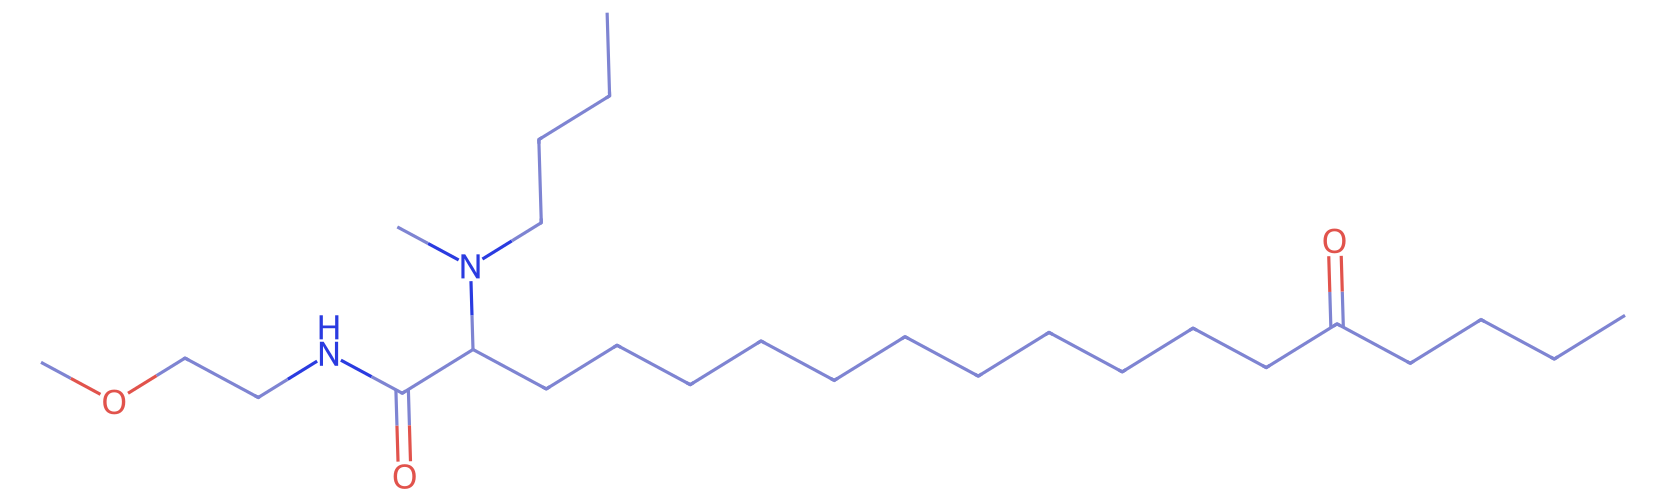
\includegraphics[width=\linewidth,height=\atlasgraphheight,keepaspectratio]{figures/forge_generated_sample_atlas_v1/forge_generated_atlas_row_01_2d.png}
\par\vspace{\atlassmilesskip}
{\atlassmilesstyle CCCCC(=O)CCCCCCCCCCCC(C(=O)N\allowbreak{}CCOC)N(C)CCCC\par}
\end{minipage}
&
\begin{minipage}[c][\atlasrowheight][c]{\atlasviewwidth}
\centering
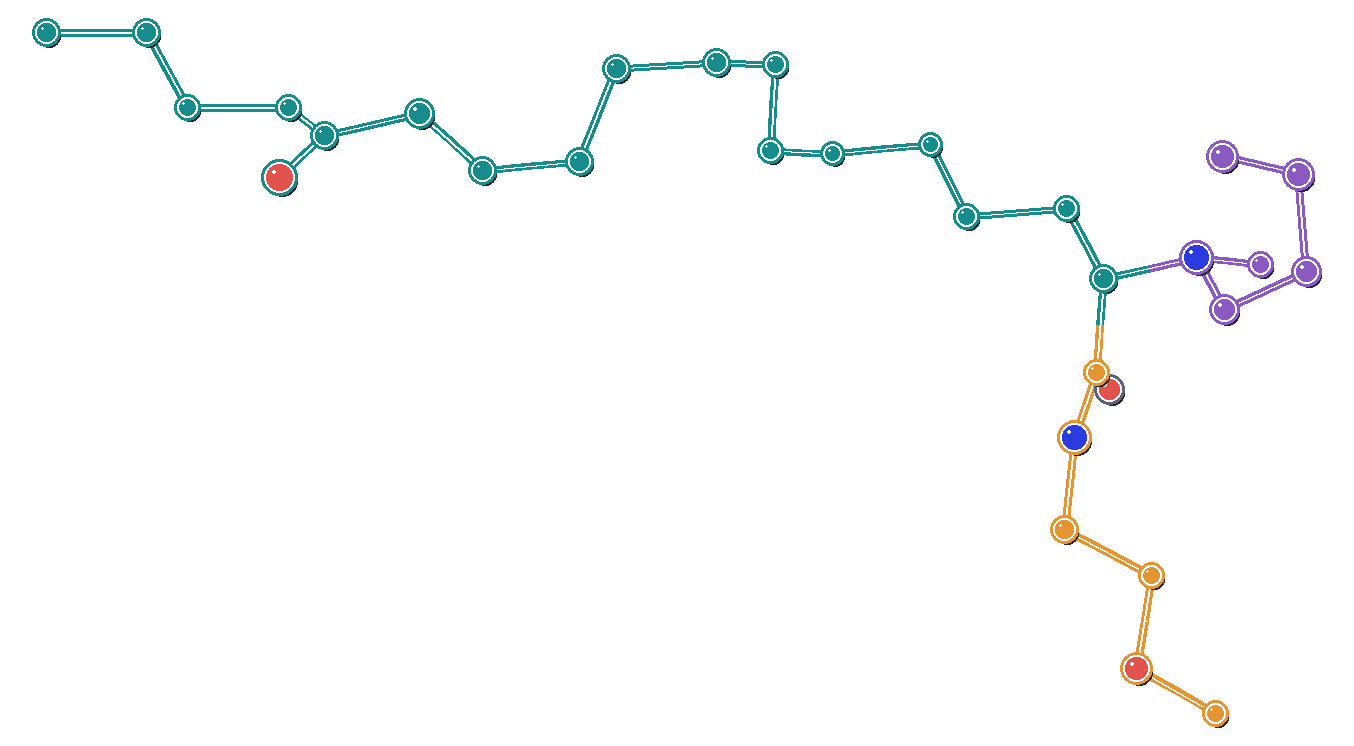
\includegraphics[width=\linewidth,height=\atlasviewheight,keepaspectratio]{figures/forge_generated_sample_atlas_v1/forge_generated_atlas_row_01_3d.png}
\end{minipage}\\
\atlasrank{2}
&
\begin{minipage}[c][\atlasrowheight][c]{\atlasgraphwidth}
\centering
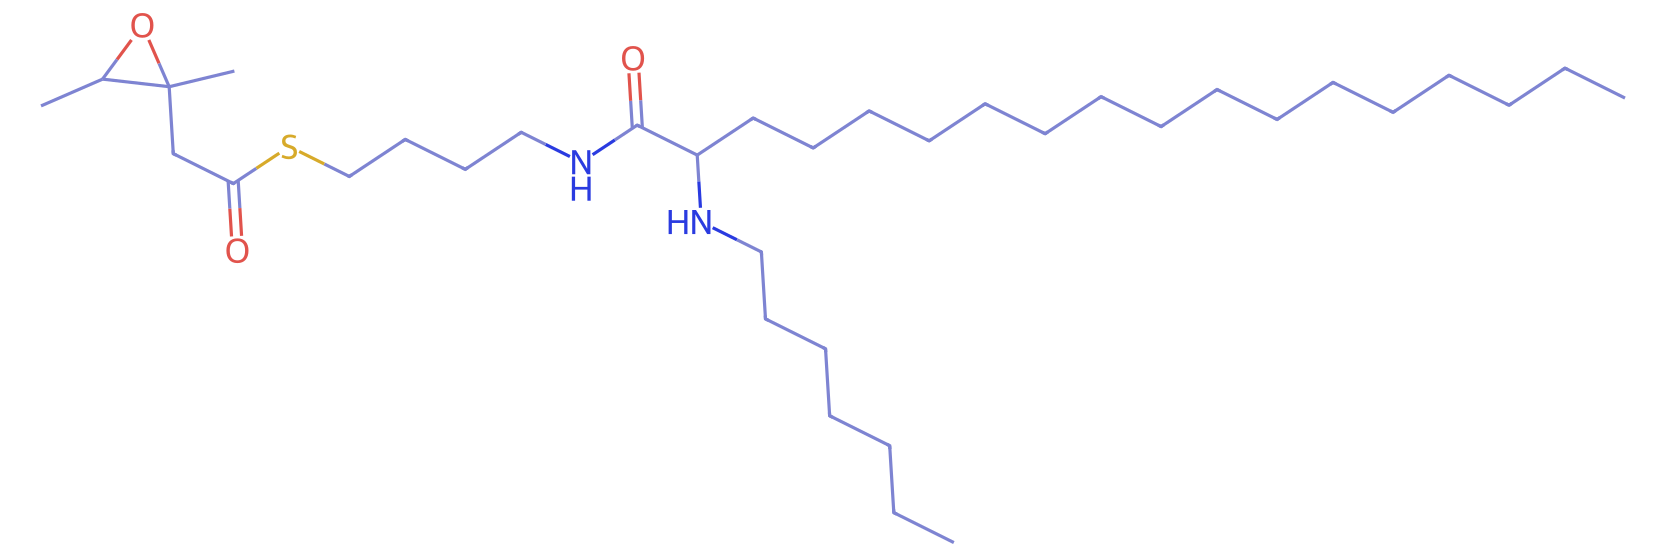
\includegraphics[width=\linewidth,height=\atlasgraphheight,keepaspectratio]{figures/forge_generated_sample_atlas_v1/forge_generated_atlas_row_02_2d.png}
\par\vspace{\atlassmilesskip}
{\atlassmilesstyle CCCCCCCCCCCCCCCCC(NCCCCCCC)C\allowbreak{}(=O)NCCCCSC(=O)CC1(C)OC1C\par}
\end{minipage}
&
\begin{minipage}[c][\atlasrowheight][c]{\atlasviewwidth}
\centering
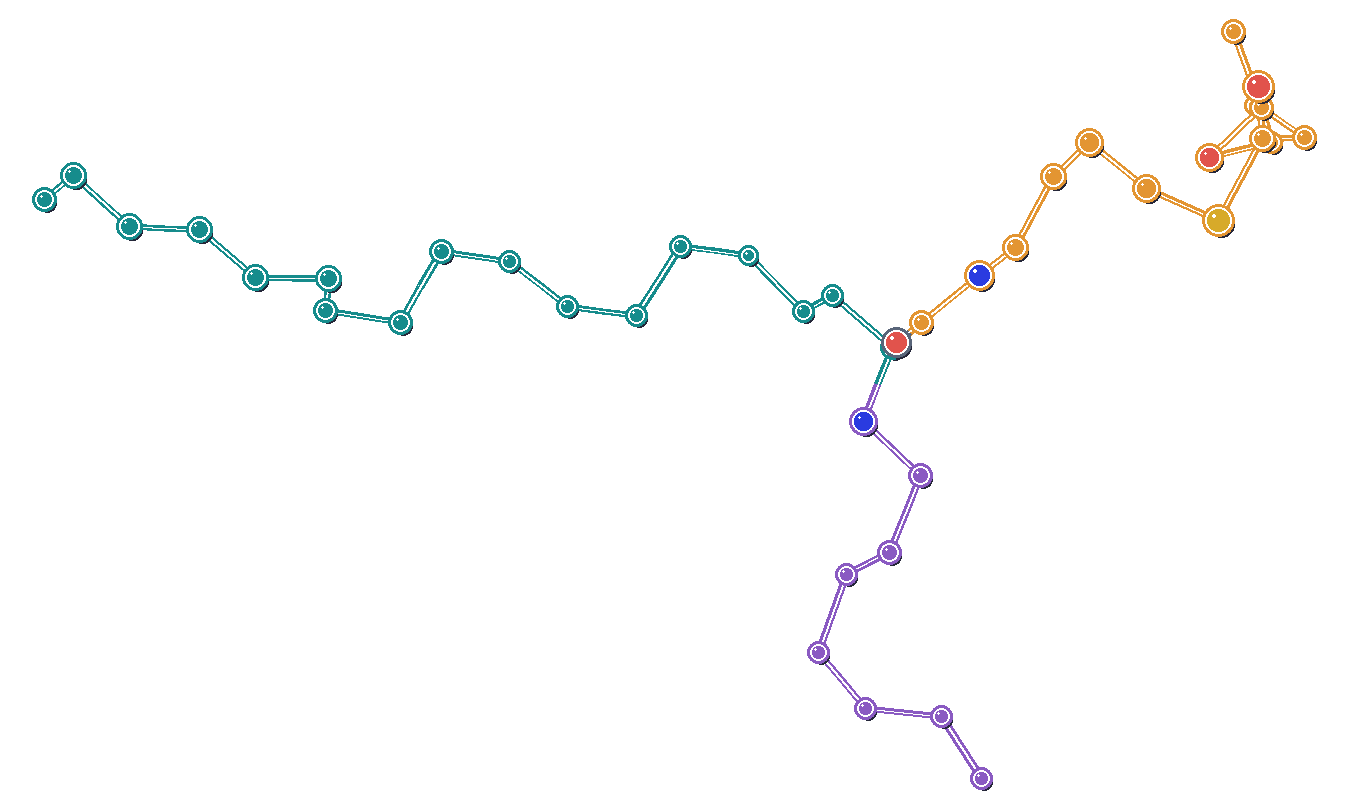
\includegraphics[width=\linewidth,height=\atlasviewheight,keepaspectratio]{figures/forge_generated_sample_atlas_v1/forge_generated_atlas_row_02_3d.png}
\end{minipage}\\
\atlasrank{3}
&
\begin{minipage}[c][\atlasrowheight][c]{\atlasgraphwidth}
\centering
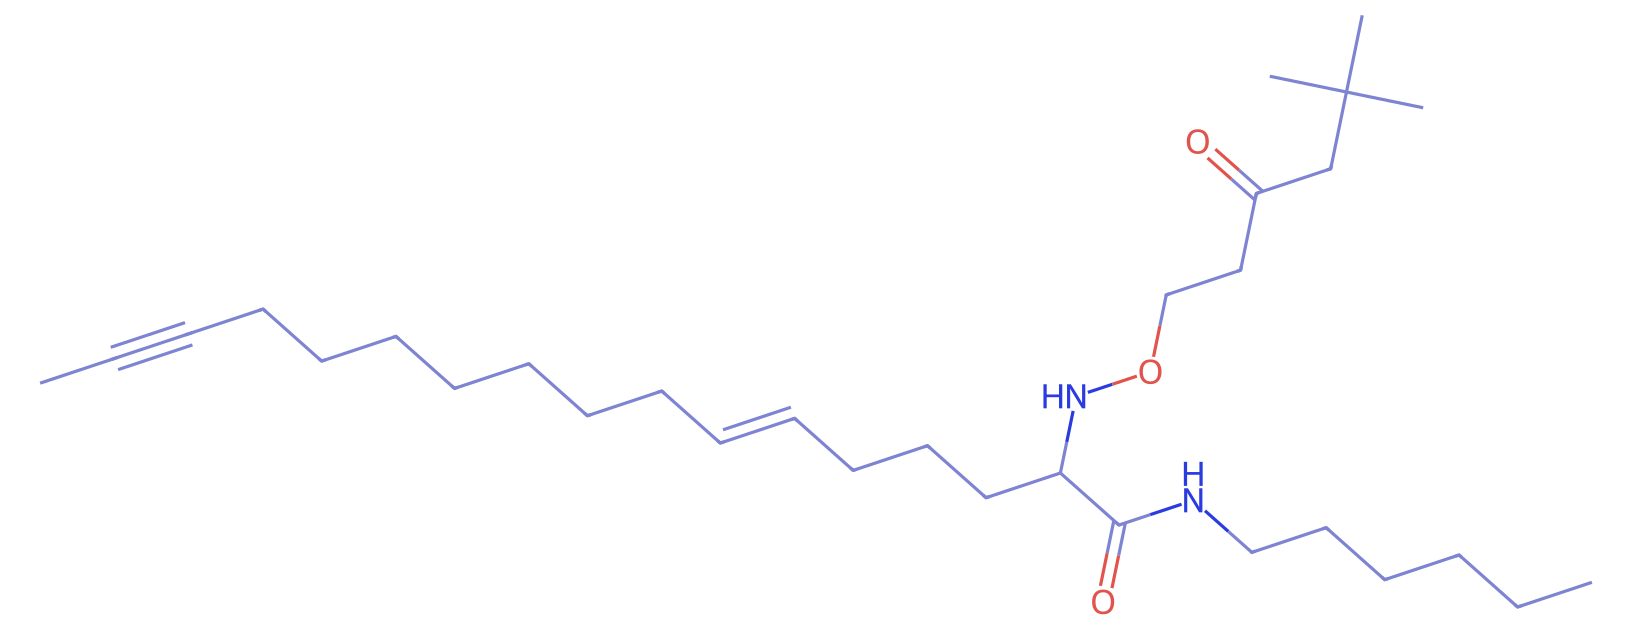
\includegraphics[width=\linewidth,height=\atlasgraphheight,keepaspectratio]{figures/forge_generated_sample_atlas_v1/forge_generated_atlas_row_03_2d.png}
\par\vspace{\atlassmilesskip}
{\atlassmilesstyle CC\#CCCCCCCCC=CCCCC(NOCCC(=O)\allowbreak{}CC(C)(C)C)C(=O)NCCCCCC\par}
\end{minipage}
&
\begin{minipage}[c][\atlasrowheight][c]{\atlasviewwidth}
\centering
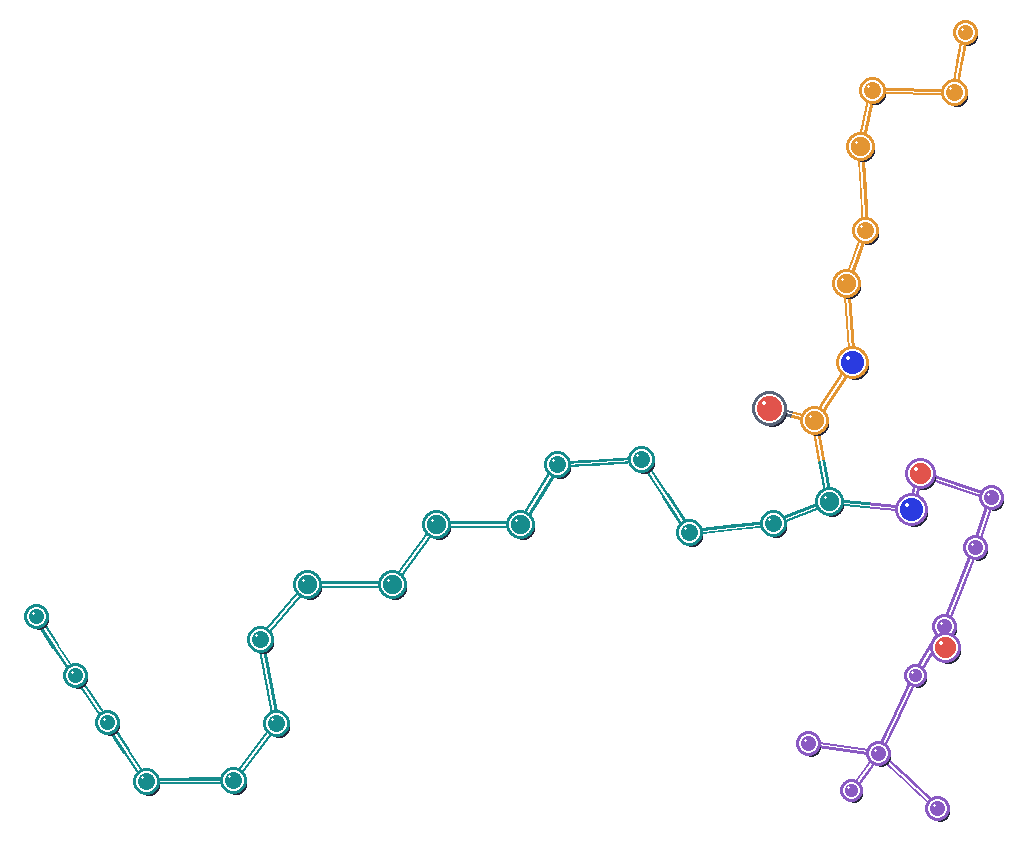
\includegraphics[width=\linewidth,height=\atlasviewheight,keepaspectratio]{figures/forge_generated_sample_atlas_v1/forge_generated_atlas_row_03_3d.png}
\end{minipage}\\
\atlasrank{4}
&
\begin{minipage}[c][\atlasrowheight][c]{\atlasgraphwidth}
\centering
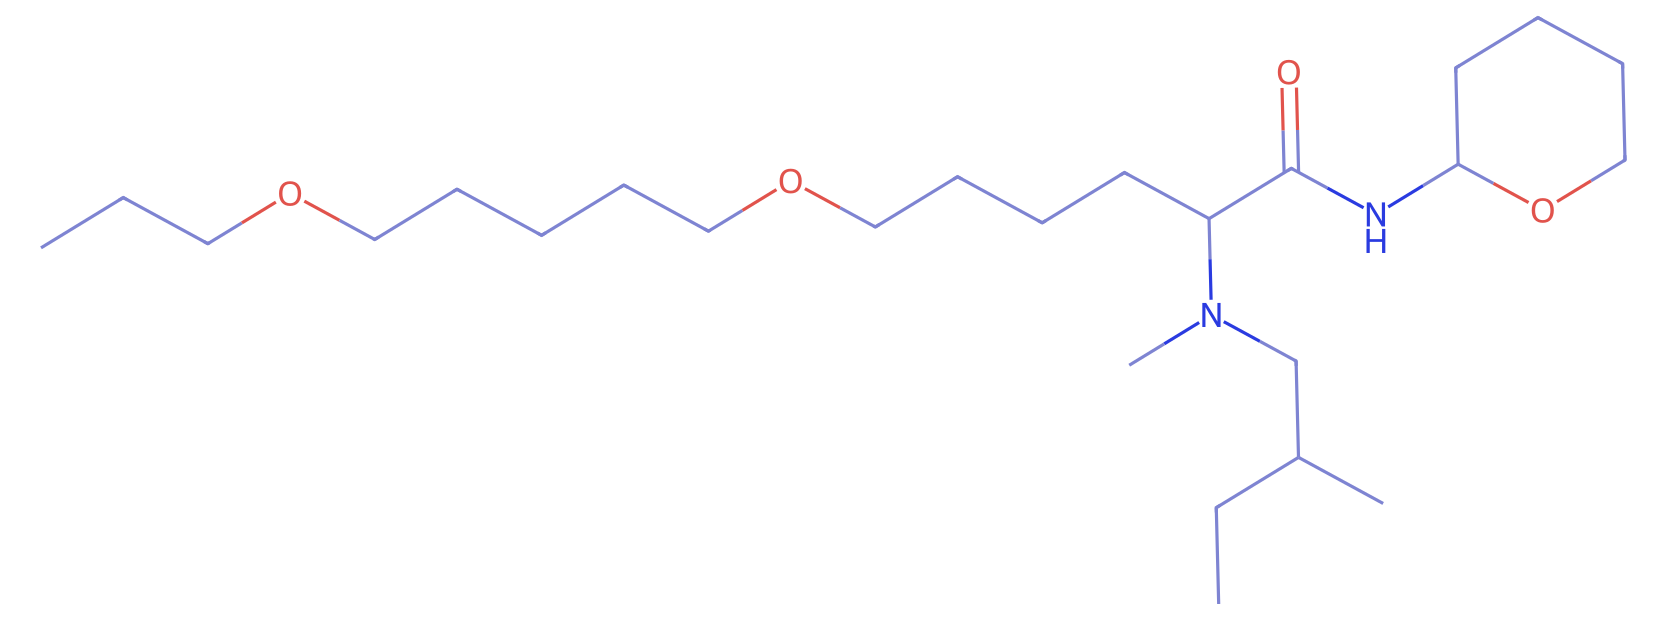
\includegraphics[width=\linewidth,height=\atlasgraphheight,keepaspectratio]{figures/forge_generated_sample_atlas_v1/forge_generated_atlas_row_04_2d.png}
\par\vspace{\atlassmilesskip}
{\atlassmilesstyle CCCOCCCCCOCCCCC(C(=O)NC1CCCC\allowbreak{}O1)N(C)CC(C)CC\par}
\end{minipage}
&
\begin{minipage}[c][\atlasrowheight][c]{\atlasviewwidth}
\centering
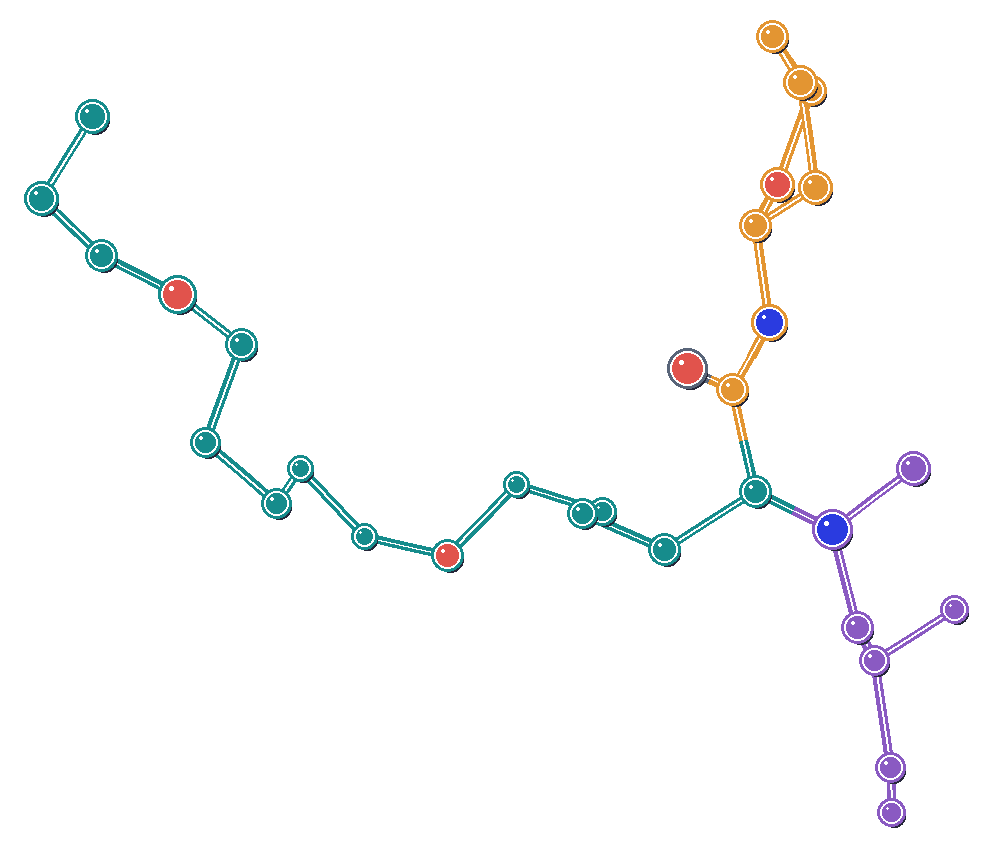
\includegraphics[width=\linewidth,height=\atlasviewheight,keepaspectratio]{figures/forge_generated_sample_atlas_v1/forge_generated_atlas_row_04_3d.png}
\end{minipage}\\
\atlasrank{5}
&
\begin{minipage}[c][\atlasrowheight][c]{\atlasgraphwidth}
\centering
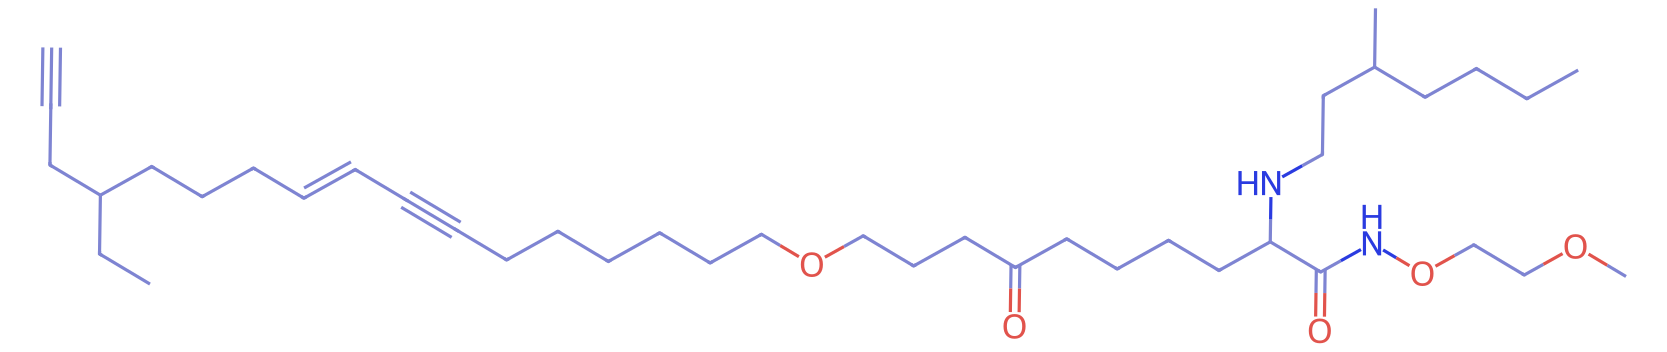
\includegraphics[width=\linewidth,height=\atlasgraphheight,keepaspectratio]{figures/forge_generated_sample_atlas_v1/forge_generated_atlas_row_05_2d.png}
\par\vspace{\atlassmilesskip}
{\atlassmilesstyle C\#CCC(CC)CCCC=CC\#CCCCCCCOCCC\allowbreak{}C(=O)CCCCC(NCCC(C)CCCC)C(=O)\allowbreak{}NOCCOC\par}
\end{minipage}
&
\begin{minipage}[c][\atlasrowheight][c]{\atlasviewwidth}
\centering
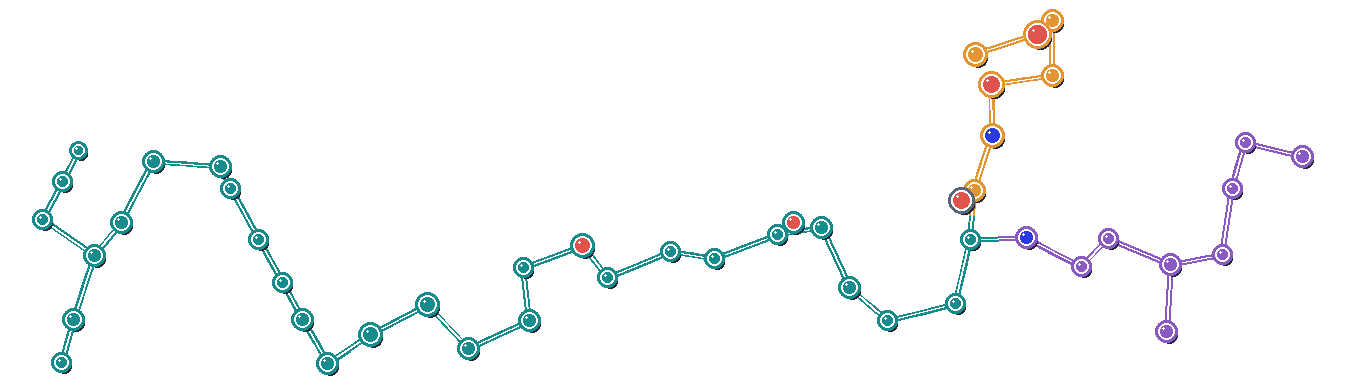
\includegraphics[width=\linewidth,height=\atlasviewheight,keepaspectratio]{figures/forge_generated_sample_atlas_v1/forge_generated_atlas_row_05_3d.png}
\end{minipage}\\
\atlasrank{6}
&
\begin{minipage}[c][\atlasrowheight][c]{\atlasgraphwidth}
\centering
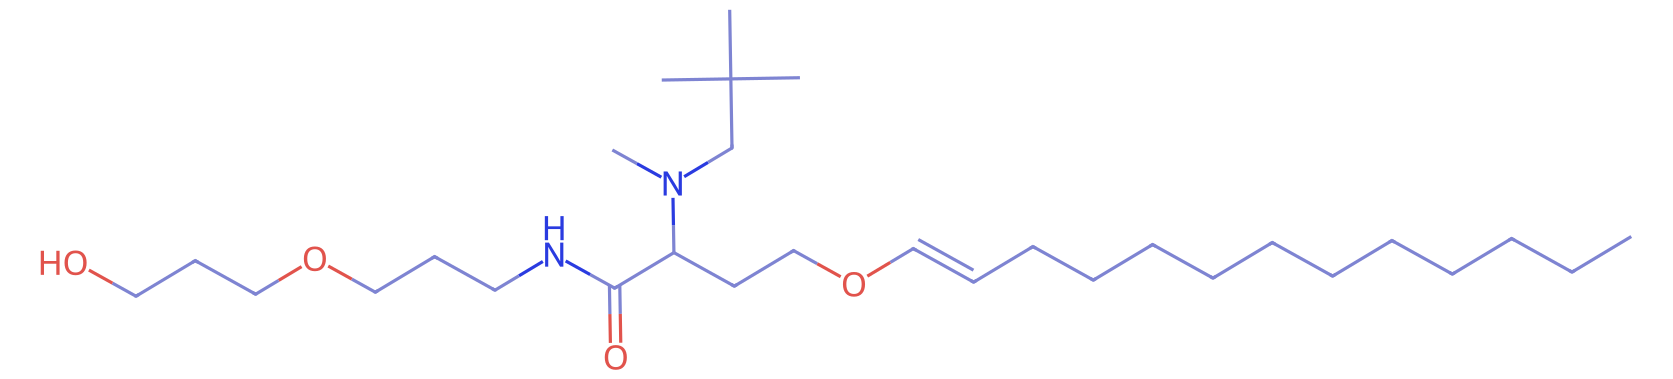
\includegraphics[width=\linewidth,height=\atlasgraphheight,keepaspectratio]{figures/forge_generated_sample_atlas_v1/forge_generated_atlas_row_06_2d.png}
\par\vspace{\atlassmilesskip}
{\atlassmilesstyle CCCCCCCCCCCC=COCCC(C(=O)NCCC\allowbreak{}OCCCO)N(C)CC(C)(C)C\par}
\end{minipage}
&
\begin{minipage}[c][\atlasrowheight][c]{\atlasviewwidth}
\centering
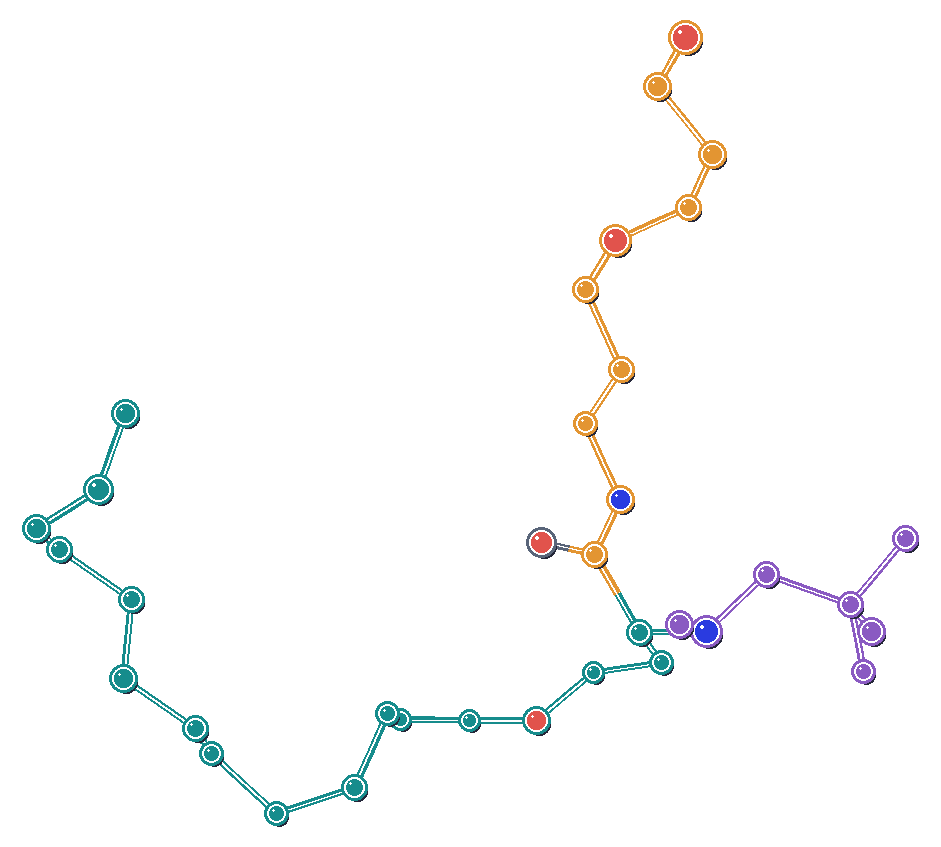
\includegraphics[width=\linewidth,height=\atlasviewheight,keepaspectratio]{figures/forge_generated_sample_atlas_v1/forge_generated_atlas_row_06_3d.png}
\end{minipage}\\
\atlasrank{7}
&
\begin{minipage}[c][\atlasrowheight][c]{\atlasgraphwidth}
\centering
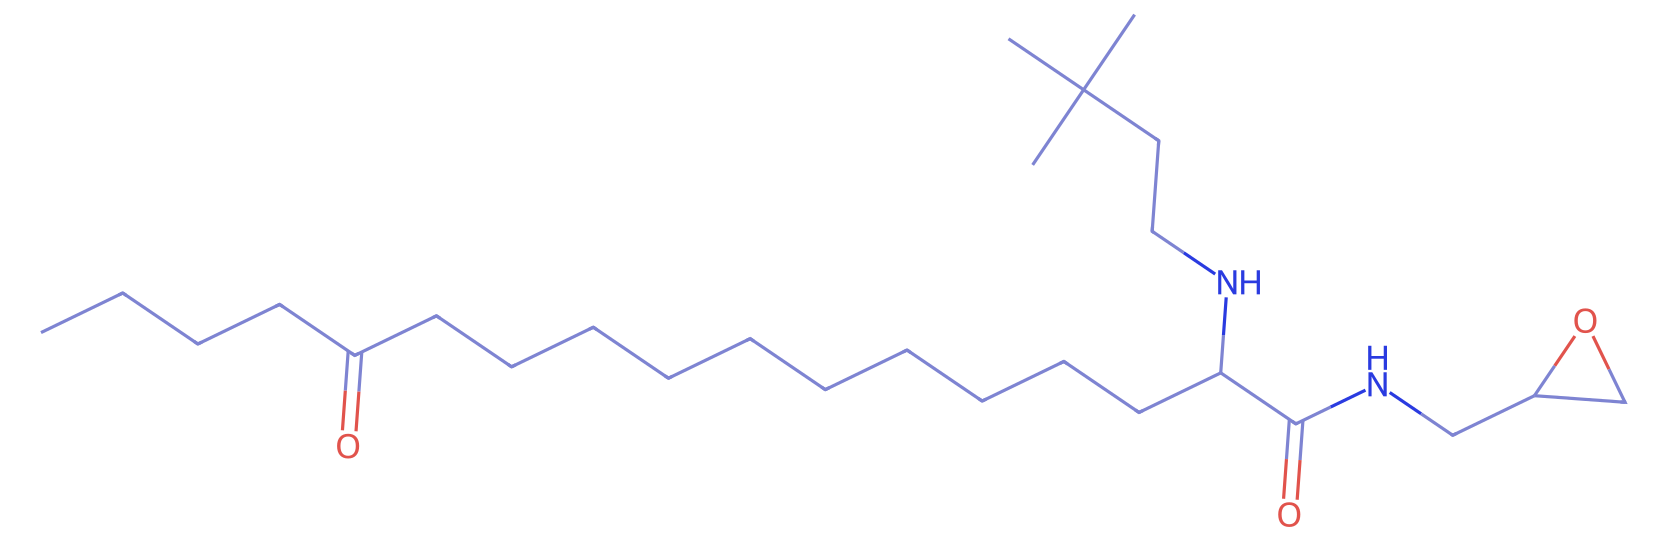
\includegraphics[width=\linewidth,height=\atlasgraphheight,keepaspectratio]{figures/forge_generated_sample_atlas_v1/forge_generated_atlas_row_07_2d.png}
\par\vspace{\atlassmilesskip}
{\atlassmilesstyle CCCCC(=O)CCCCCCCCCCC(NCCC(C)\allowbreak{}(C)C)C(=O)NCC1CO1\par}
\end{minipage}
&
\begin{minipage}[c][\atlasrowheight][c]{\atlasviewwidth}
\centering
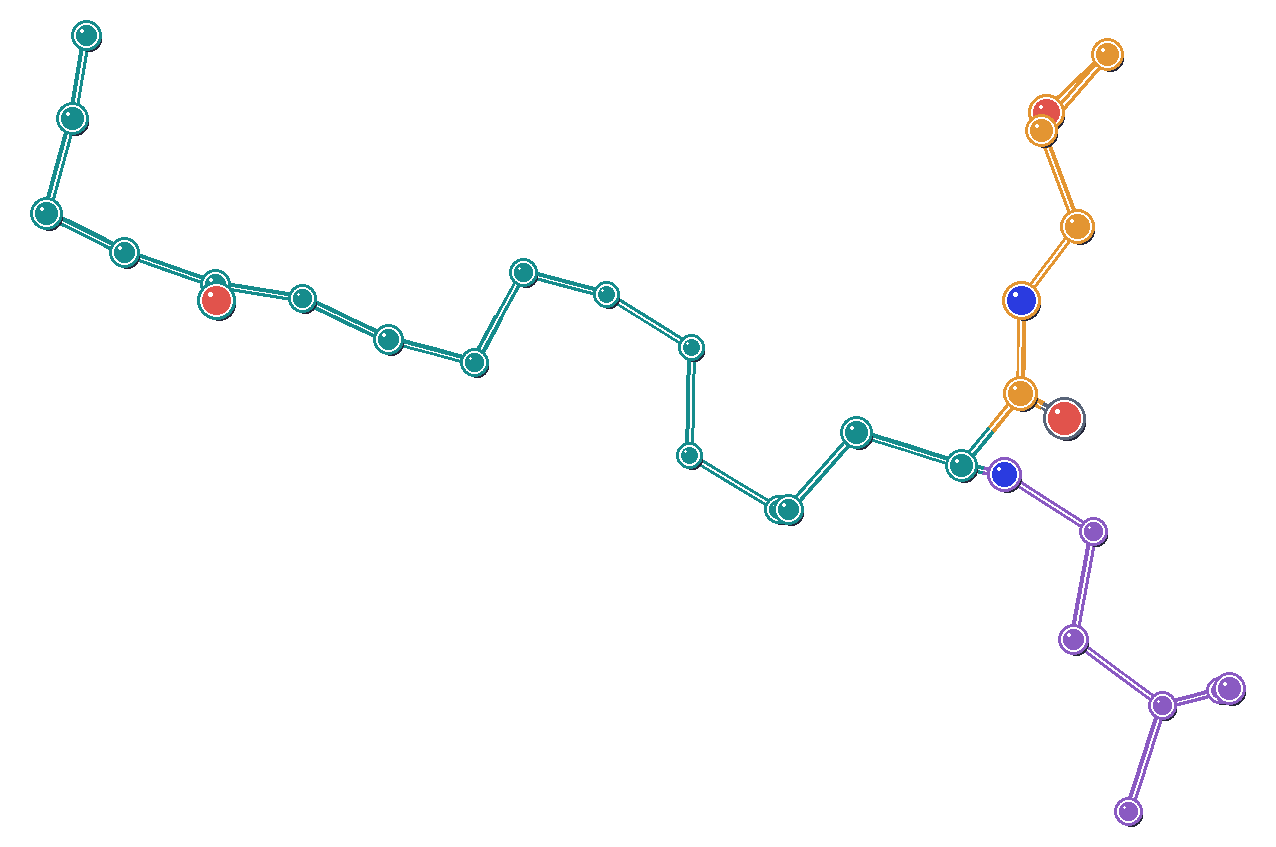
\includegraphics[width=\linewidth,height=\atlasviewheight,keepaspectratio]{figures/forge_generated_sample_atlas_v1/forge_generated_atlas_row_07_3d.png}
\end{minipage}\\
\atlasrank{8}
&
\begin{minipage}[c][\atlasrowheight][c]{\atlasgraphwidth}
\centering
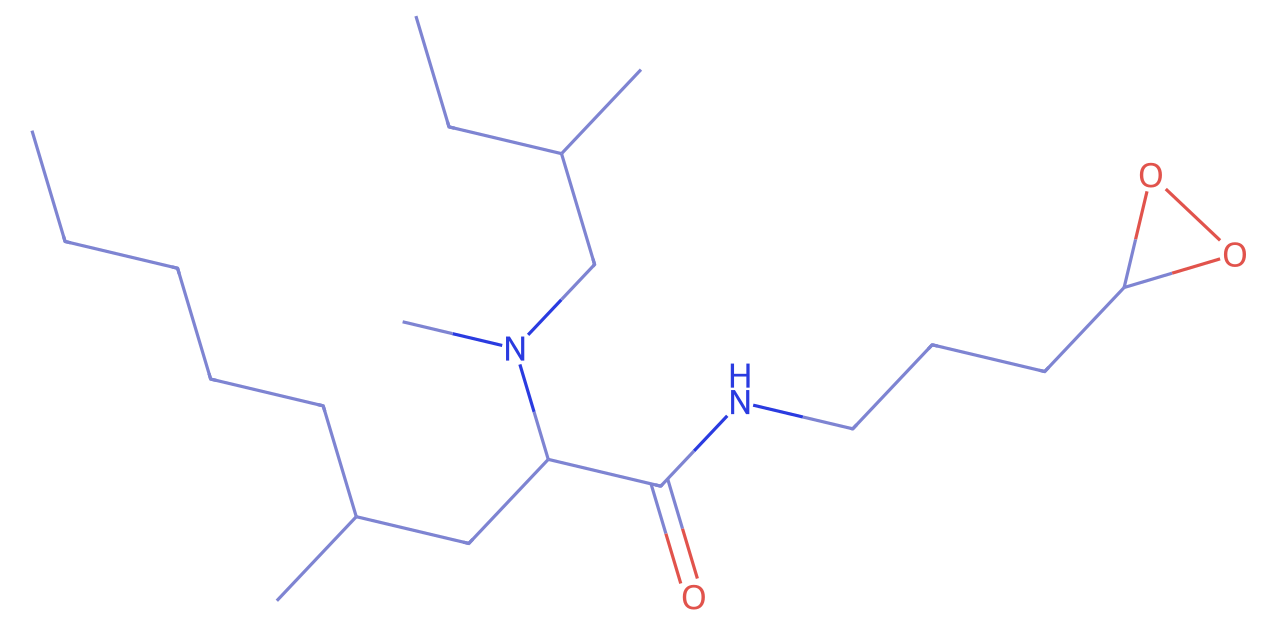
\includegraphics[width=\linewidth,height=\atlasgraphheight,keepaspectratio]{figures/forge_generated_sample_atlas_v1/forge_generated_atlas_row_08_2d.png}
\par\vspace{\atlassmilesskip}
{\atlassmilesstyle CCCCCC(C)CC(C(=O)NCCCC1OO1)N\allowbreak{}(C)CC(C)CC\par}
\end{minipage}
&
\begin{minipage}[c][\atlasrowheight][c]{\atlasviewwidth}
\centering
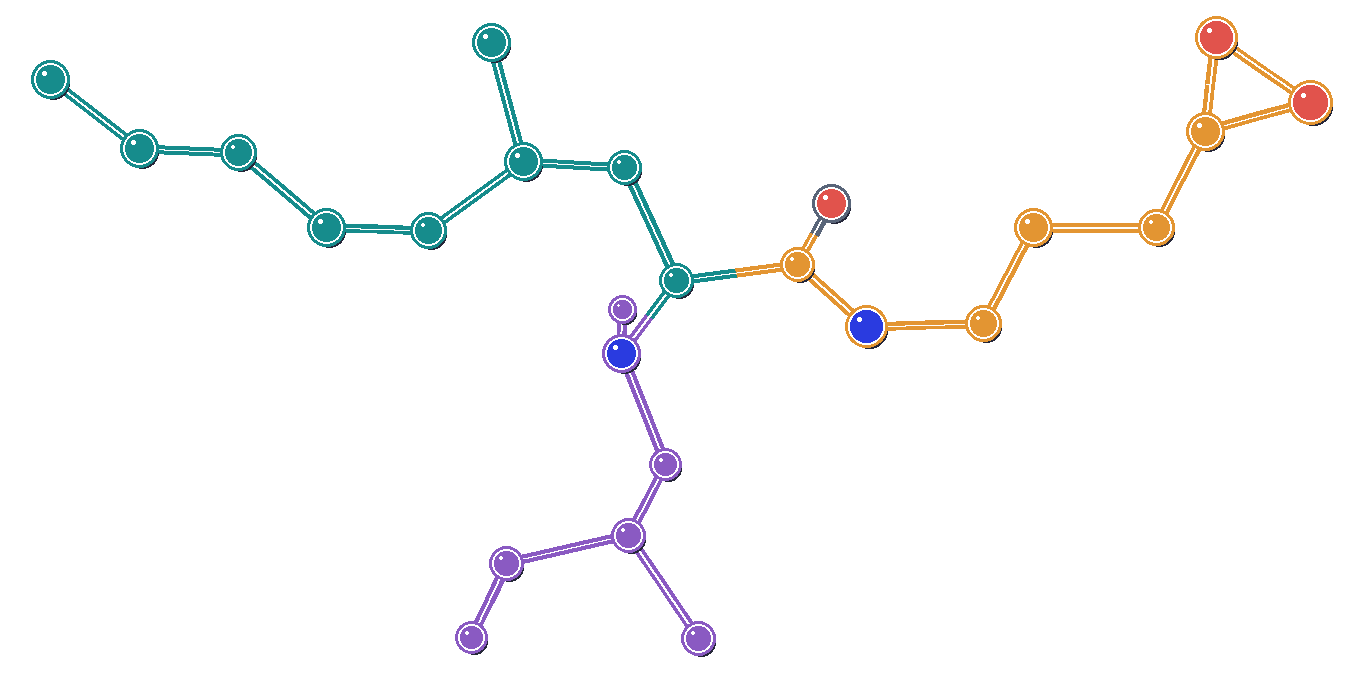
\includegraphics[width=\linewidth,height=\atlasviewheight,keepaspectratio]{figures/forge_generated_sample_atlas_v1/forge_generated_atlas_row_08_3d.png}
\end{minipage}\\
\atlasrank{9}
&
\begin{minipage}[c][\atlasrowheight][c]{\atlasgraphwidth}
\centering
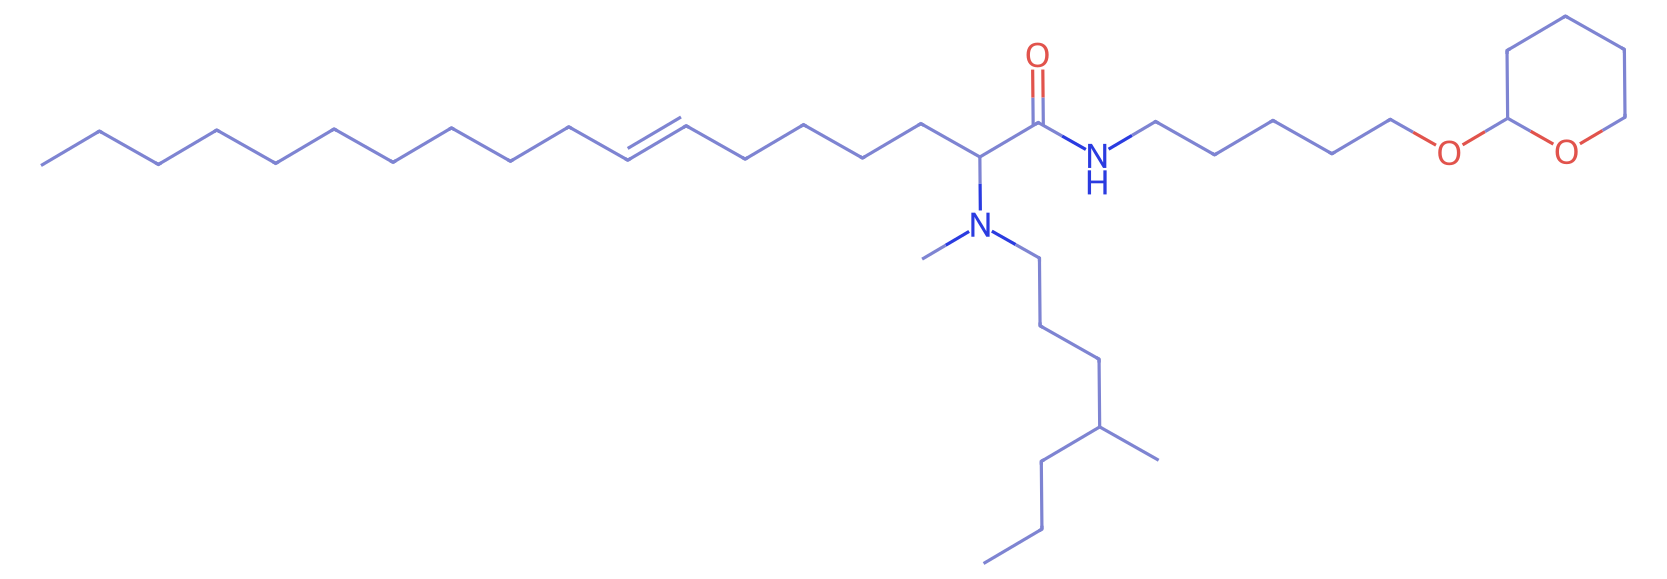
\includegraphics[width=\linewidth,height=\atlasgraphheight,keepaspectratio]{figures/forge_generated_sample_atlas_v1/forge_generated_atlas_row_09_2d.png}
\par\vspace{\atlassmilesskip}
{\atlassmilesstyle CCCCCCCCCCC=CCCCCC(C(=O)NCCC\allowbreak{}CCOC1CCCCO1)N(C)CCCC(C)CCC\par}
\end{minipage}
&
\begin{minipage}[c][\atlasrowheight][c]{\atlasviewwidth}
\centering
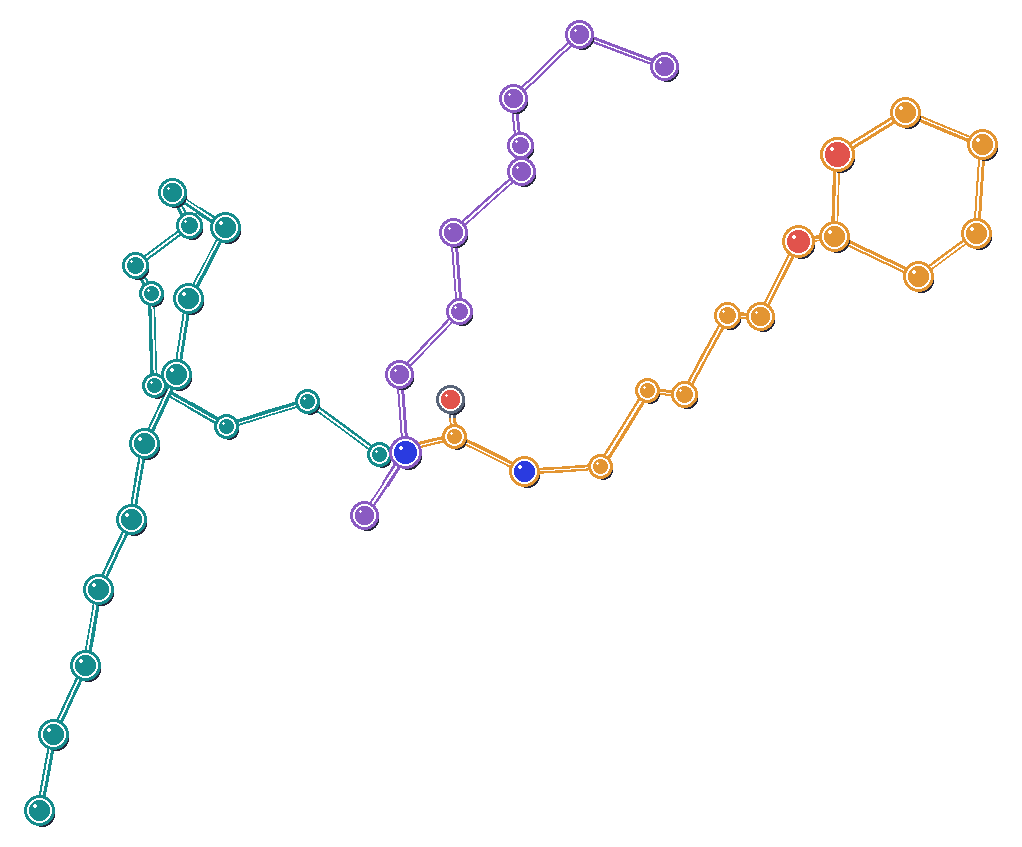
\includegraphics[width=\linewidth,height=\atlasviewheight,keepaspectratio]{figures/forge_generated_sample_atlas_v1/forge_generated_atlas_row_09_3d.png}
\end{minipage}\\
\atlasrank{10}
&
\begin{minipage}[c][\atlasrowheight][c]{\atlasgraphwidth}
\centering
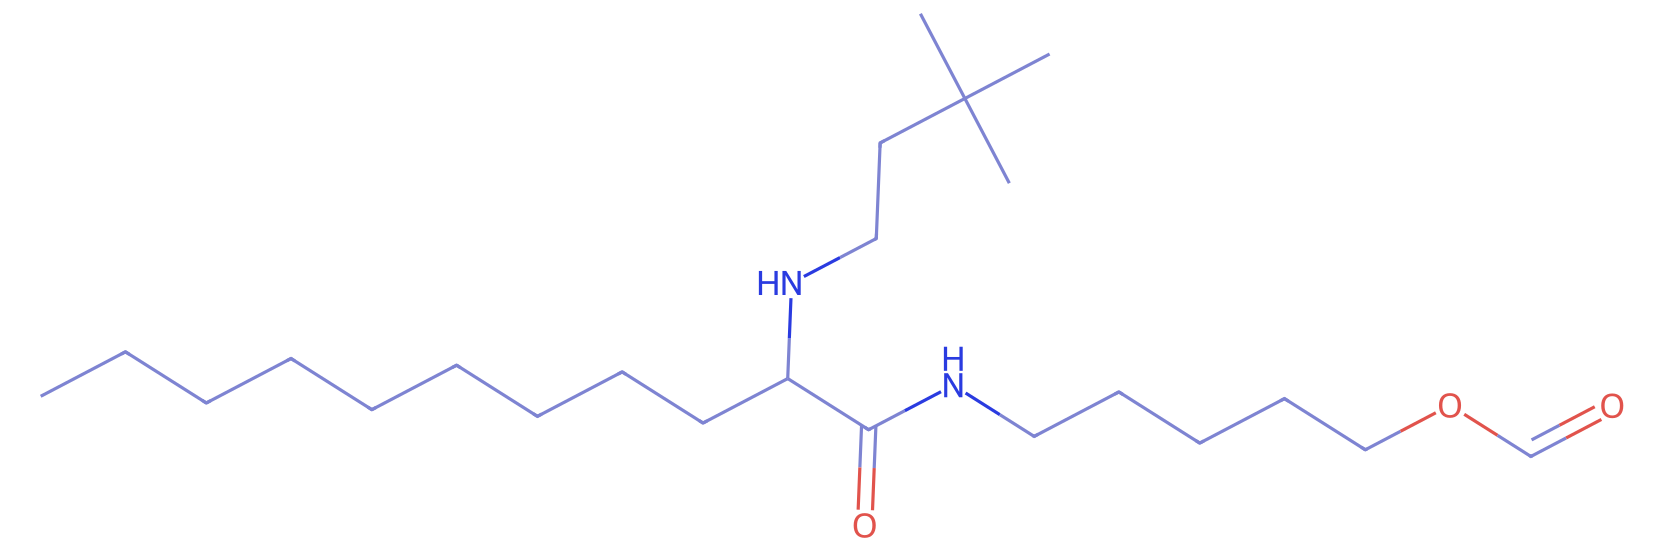
\includegraphics[width=\linewidth,height=\atlasgraphheight,keepaspectratio]{figures/forge_generated_sample_atlas_v1/forge_generated_atlas_row_10_2d.png}
\par\vspace{\atlassmilesskip}
{\atlassmilesstyle CCCCCCCCCC(NCCC(C)(C)C)C(=O)\allowbreak{}NCCCCCOC=O\par}
\end{minipage}
&
\begin{minipage}[c][\atlasrowheight][c]{\atlasviewwidth}
\centering
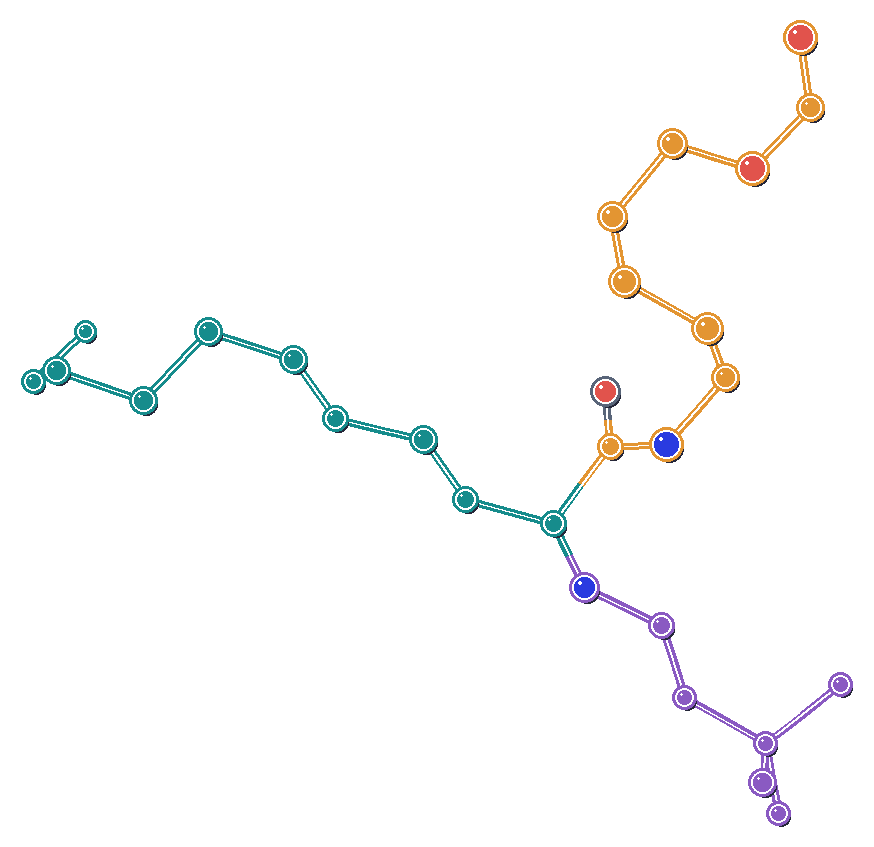
\includegraphics[width=\linewidth,height=\atlasviewheight,keepaspectratio]{figures/forge_generated_sample_atlas_v1/forge_generated_atlas_row_10_3d.png}
\end{minipage}\\
\atlasrank{11}
&
\begin{minipage}[c][\atlasrowheight][c]{\atlasgraphwidth}
\centering
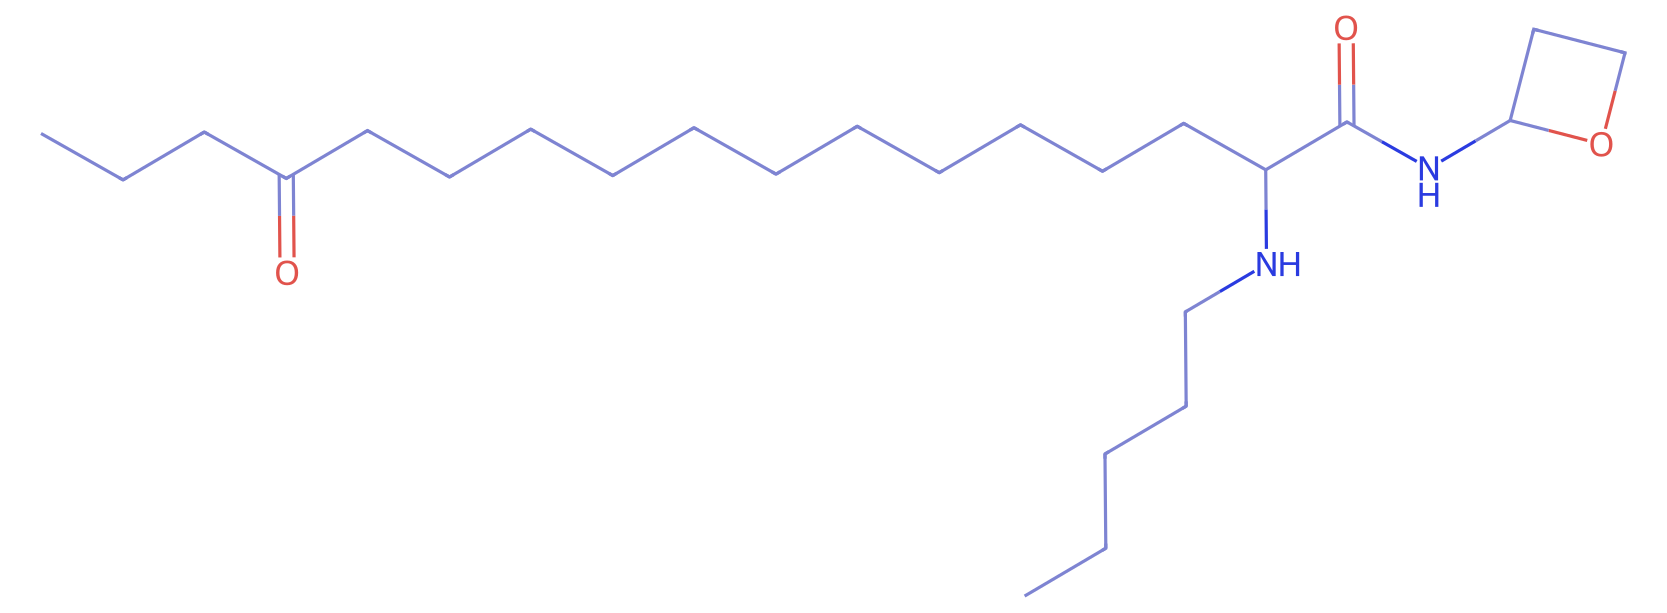
\includegraphics[width=\linewidth,height=\atlasgraphheight,keepaspectratio]{figures/forge_generated_sample_atlas_v1/forge_generated_atlas_row_11_2d.png}
\par\vspace{\atlassmilesskip}
{\atlassmilesstyle CCCCCNC(CCCCCCCCCCCC(=O)CCC)\allowbreak{}C(=O)NC1CCO1\par}
\end{minipage}
&
\begin{minipage}[c][\atlasrowheight][c]{\atlasviewwidth}
\centering
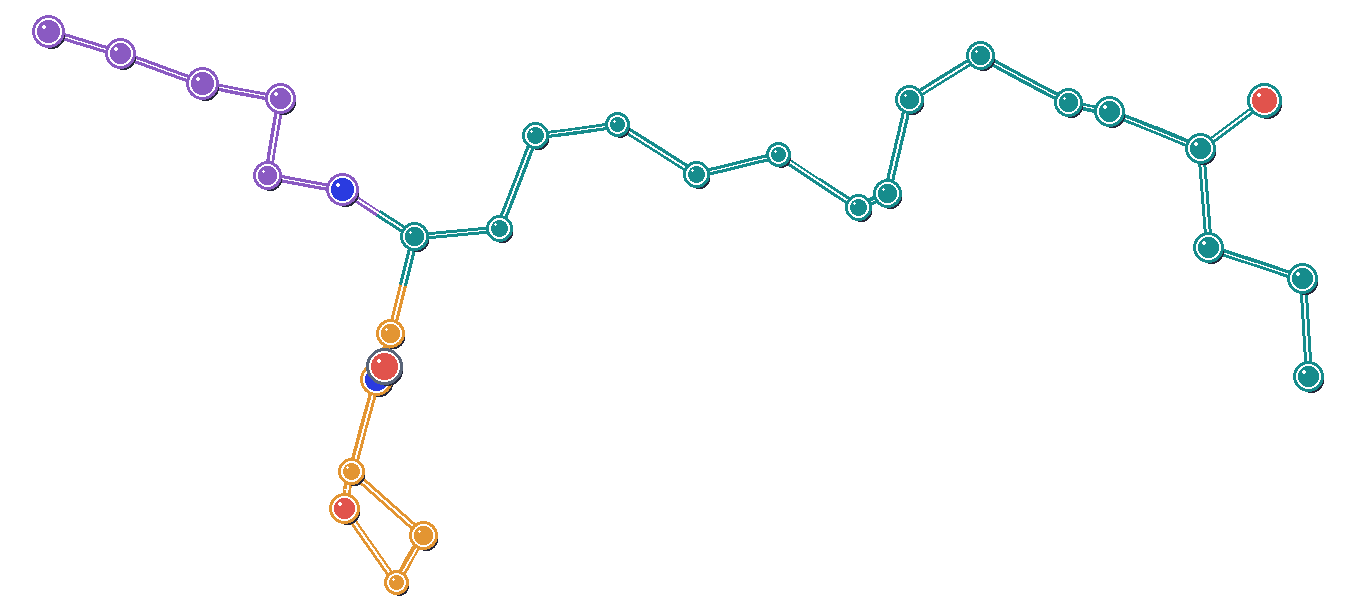
\includegraphics[width=\linewidth,height=\atlasviewheight,keepaspectratio]{figures/forge_generated_sample_atlas_v1/forge_generated_atlas_row_11_3d.png}
\end{minipage}\\
\atlasrank{12}
&
\begin{minipage}[c][\atlasrowheight][c]{\atlasgraphwidth}
\centering
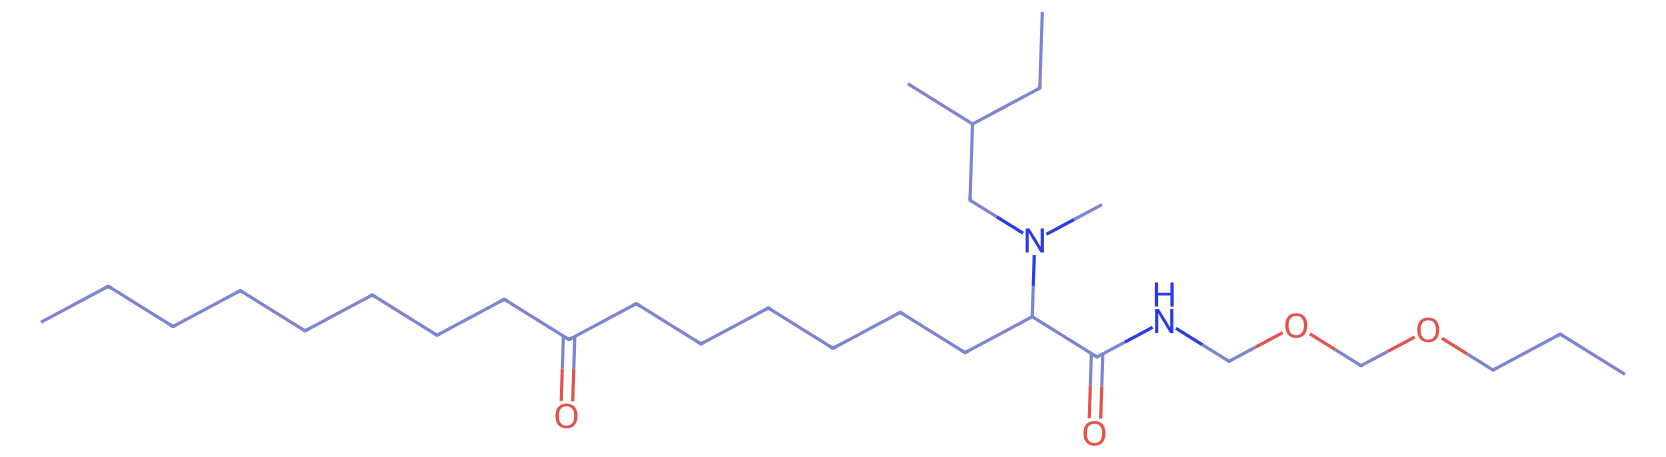
\includegraphics[width=\linewidth,height=\atlasgraphheight,keepaspectratio]{figures/forge_generated_sample_atlas_v1/forge_generated_atlas_row_12_2d.png}
\par\vspace{\atlassmilesskip}
{\atlassmilesstyle CCCCCCCCC(=O)CCCCCCC(C(=O)NC\allowbreak{}OCOCCC)N(C)CC(C)CC\par}
\end{minipage}
&
\begin{minipage}[c][\atlasrowheight][c]{\atlasviewwidth}
\centering
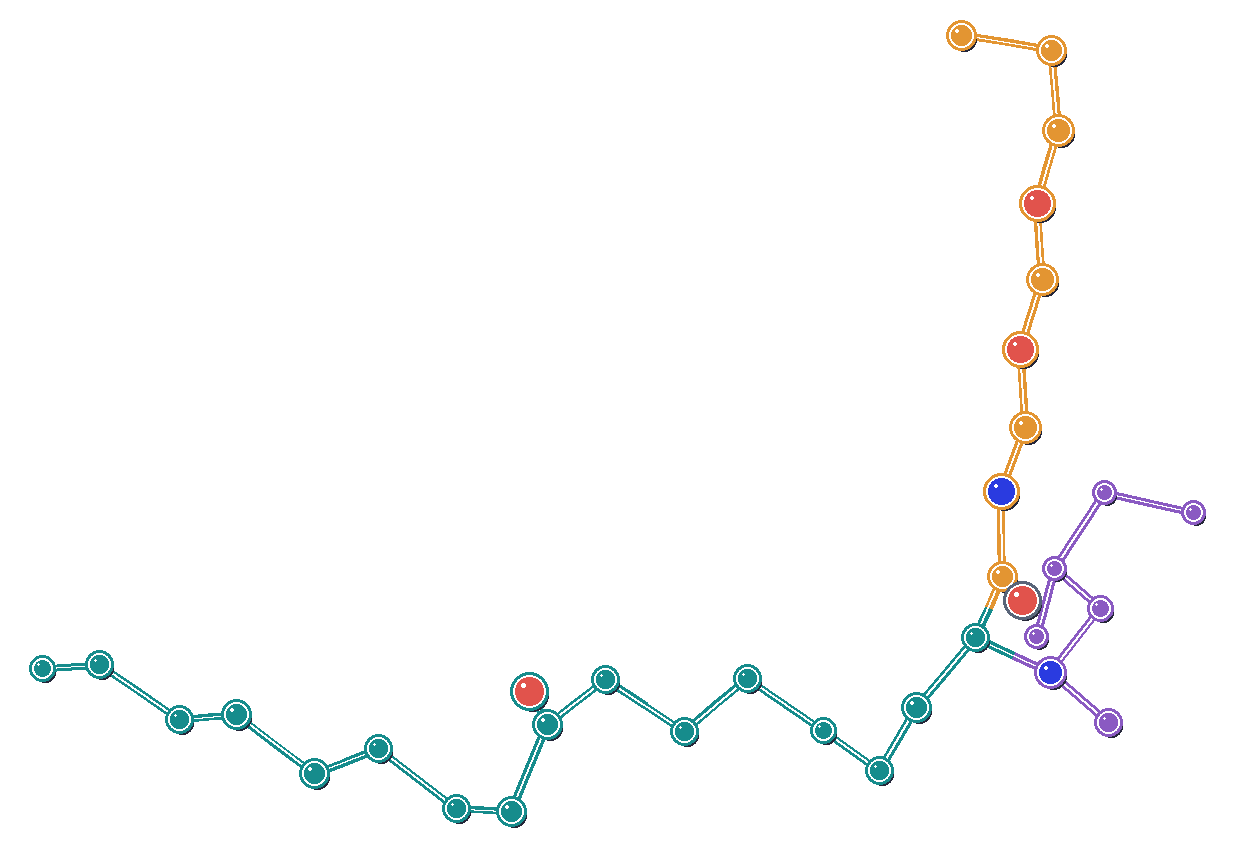
\includegraphics[width=\linewidth,height=\atlasviewheight,keepaspectratio]{figures/forge_generated_sample_atlas_v1/forge_generated_atlas_row_12_3d.png}
\end{minipage}\\
%
\end{longtable}
\endgroup


\end{document}
